%%%%%%%%%%%%%%%%%%%%%%%%%%%%%%%%%%%%%%%%%%%%%%%%%%%%%%%%%%%%%%%%%%%%%%%%%%%
%%
%%  tesis.tex
%%
%%  Created: Fri Oct 10 14:24:37 1997
%%  Author.: Jose Carlos Gonzalez
%%  Notes..:
%%          
%%-------------------------------------------------------------------------
%% Filename: $RCSfile$
%% Revision: $Revision$
%% Date:     $Date$
%%%%%%%%%%%%%%%%%%%%%%%%%%%%%%%%%%%%%%%%%%%%%%%%%%%%%%%%%%%%%%%%%%%%%%%%%%%

%\usepackage[1,7-9,11-13,15-16,19-24,29-37,39-42,45-56,59-85]{pagesel}

\usepackage{prelim2e}

\typeout{----> TESIS compilation (\jobname.tex) . . .}

\listfiles

\ifpdf
  \pdfcatalog{/AcroForm<</Fields[]/NeedAppearances true>>}
\fi

\input{language.tex}

\COLORversionfalse

%======================================== Paquetes y definiciones

\makeindex

%======================================== BEGIN DOCUMENT

\begin{document}

%======================================== Figuras, tablas y ecuaciones

\ifpdf
  \typeout{### Precompiled for pdfLaTeX . . .}
  \DeclareGraphicsExtensions{.pdf,.mps,.jpg,.png}
\else
  \typeout{### Precompiled for LaTeX . . .}
  \DeclareGraphicsExtensions{.eps,.mps,.jpg,.png}
\fi

%%%%%%%%%%%%%%%%%%%%%%%%%%%%%%%%%%%%%%%%%%%%%%%%%%%%%%%%%%%%%%%%%%%%%%%%%%%
%%
%%  figures.tex
%%
%%  Created: Mon Oct 20 14:58:56 1997
%%  Author.: Jose Carlos Gonzalez
%%  Notes..:
%%          
%%-------------------------------------------------------------------------
%% Filename: $RCSfile$
%% Revision: $Revision$
%% Date:     $Date$
%%%%%%%%%%%%%%%%%%%%%%%%%%%%%%%%%%%%%%%%%%%%%%%%%%%%%%%%%%%%%%%%%%%%%%%%%%%

%%%%%%%%%%%%%%%%%%%%%%%%%%%%%%%%%%%%%%%%%%%%%%%%%%%%%%%%%%%%
%% THE COSMIC RADIATION %%%%%%%%%%%%%%%%%%%%%%%%%%%%%%%%%%%%
%%%%%%%%%%%%%%%%%%%%%%%%%%%%%%%%%%%%%%%%%%%%%%%%%%%%%%%%%%%%
  
%%%%%%%%%%%%%%%%%%%%%%%%%%%%%%%%%%%%%%%%%%%%%%%%%%%%%%%%%%%%
\def\AGNclassificationfig{
\begin{figure}[t]
\centering
\ifenglish
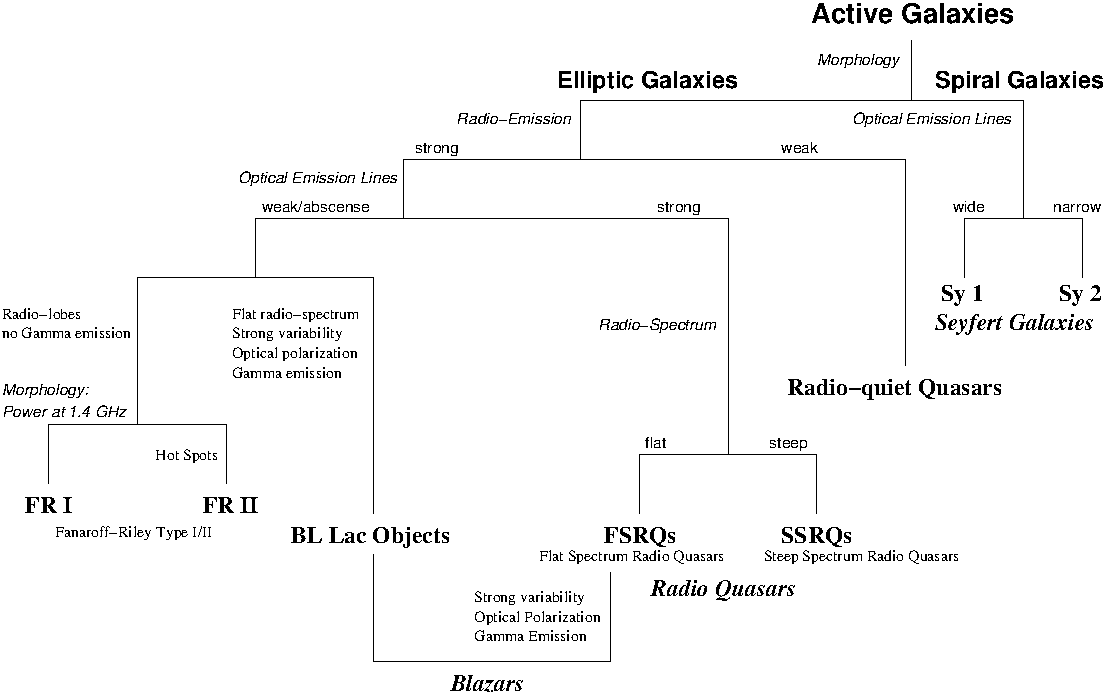
\includegraphics[width=\textwidth]{AGNclassification}
\caption[Classification of AGN family]{Classification of AGN family
  (taken from \cite{Petry:tesis})}
\else
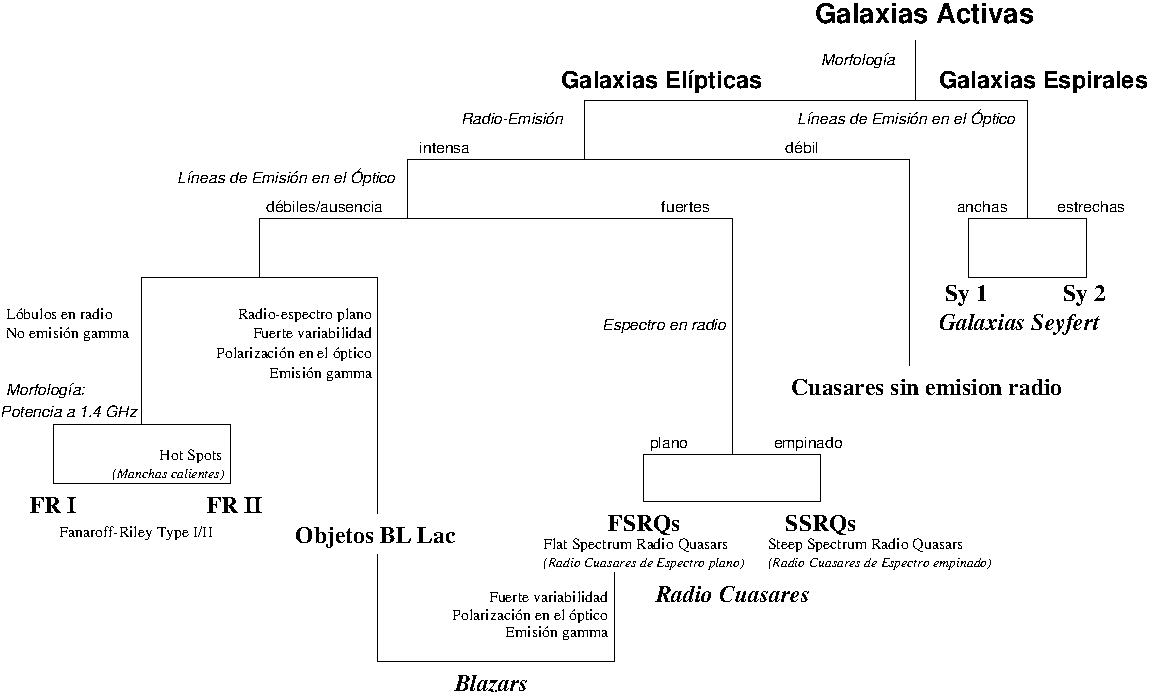
\includegraphics[width=\textwidth]{AGNclassification_e}
\caption[Classificaci'on de la familia de los AGNs]{Classificaci'on de
  la familia de los AGNs (tomado de \cite{Petry:tesis})}
\fi
\label{fig:AGNclassification}
\end{figure}
}

%%%%%%%%%%%%%%%%%%%%%%%%%%%%%%%%%%%%%%%%%%%%%%%%%%%%%%%%%%%%
\def\agnartisticviewfig{
\begin{figure}[p]
%\begin{wrapfigure}[32]{r}{0.5\textwidth}
  \centering
  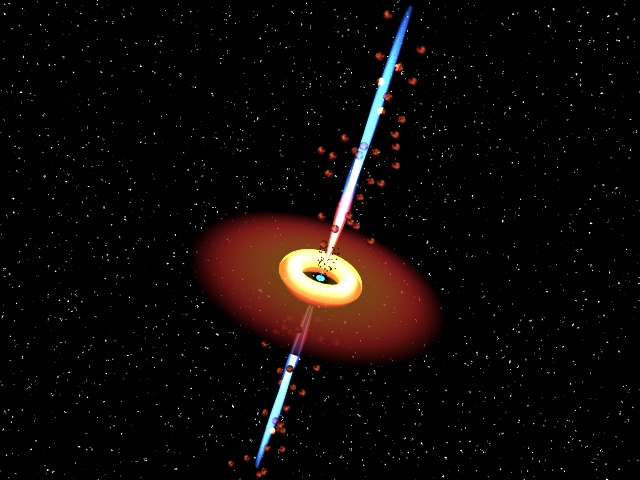
\includegraphics[height=.75\textheight]{agn}
  \ifenglish
  \caption[Artistic view of an AGN]{Artistic view of an AGN, 
    following the unified model.  The main parts are a thin, small
    accretion disk (in blue) surrounding the central black hole, a
    thick torus (in orange), two jets (for radio-loud AGN, in blue)
    and small (black) and big (red) clouds of dust.}
  \else
  \caption[Visi'on art'istica de un AGN]{Visi'on art'istica de un
    AGN, seg'un el modelo unificado. Las partes principales son un
    peque~no disco de acreci'on (en azul) en torno al agujero negro
    central, un disco grueso (en naranja), dos \emph{jets} (en AGN
    con emisi'on en radio, en azul), y nubes de gas y polvo (en
    negro y rojo).}  
  \fi
  \label{fig:agnartisticview}
\end{figure}
%\end{wrapfigure}
}

%%%%%%%%%%%%%%%%%%%%%%%%%%%%%%%%%%%%%%%%%%%%%%%%%%%%%%%%%%%%
\def\agninterpretationfig{
%\begin{figure}[htbp]
\begin{wrapfigure}[21]{r}{0.5\textwidth}
  \centering
  \ifenglish
  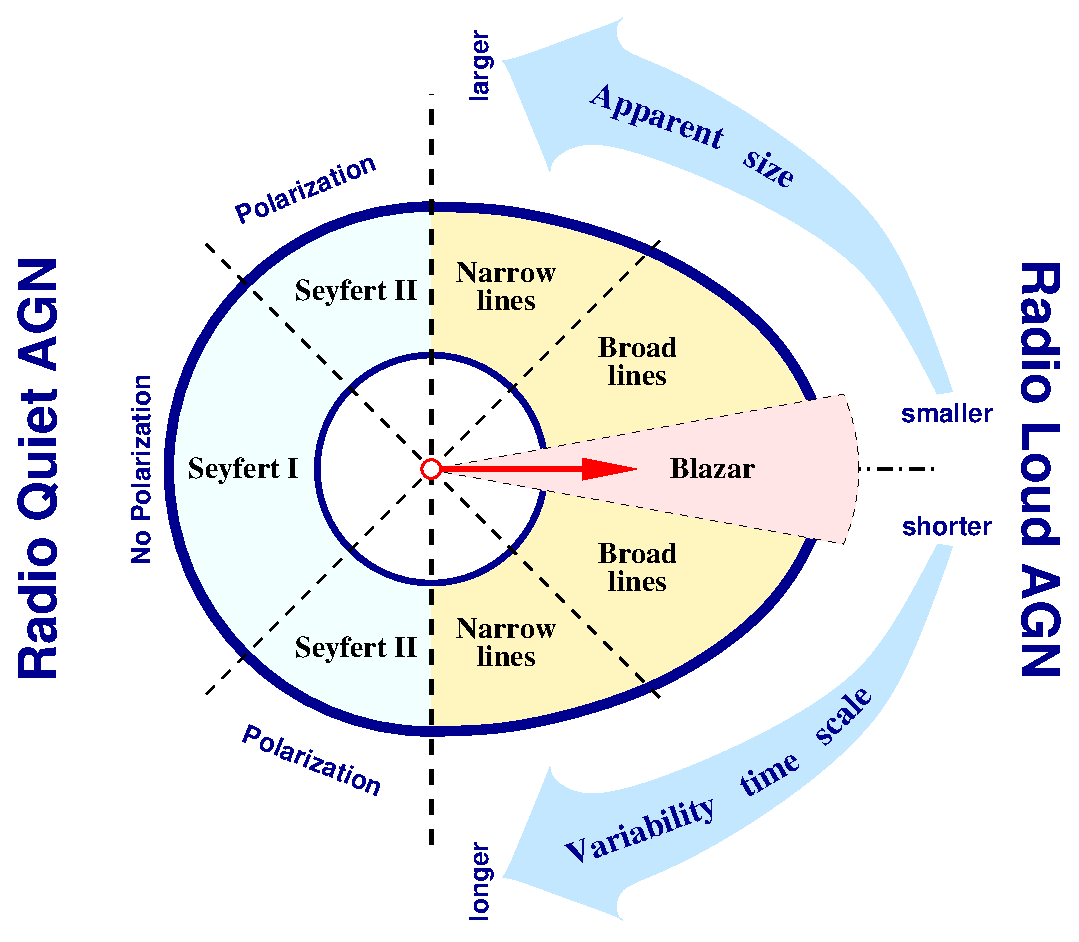
\includegraphics[width=.49\textwidth]{agninterp}
  \caption[Interpretation of the unified model of the AGN]{Schematic 
    interpretation of the unified model of the AGN.  The arrow
    indicates the direction of the jets, for radio-loud AGN (adapted
    from \cite{hoffman})} \else
  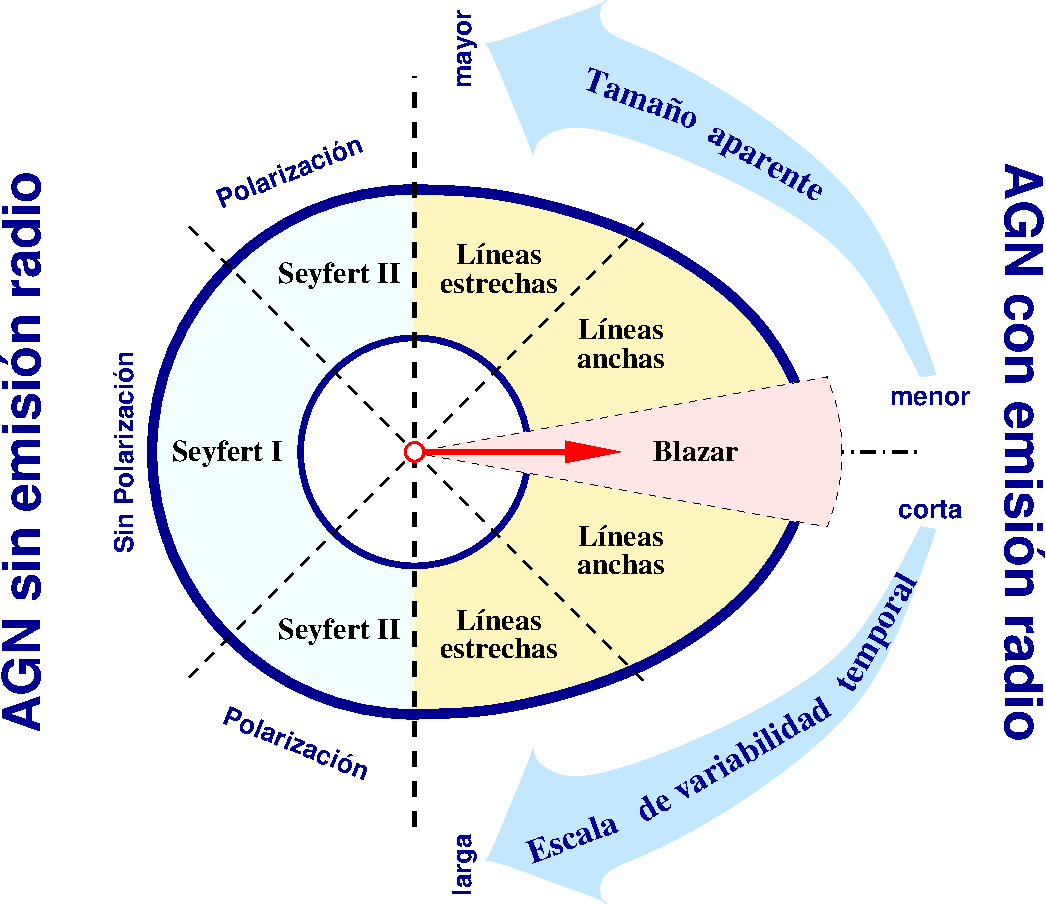
\includegraphics[width=.49\textwidth]{agninterp_e}
  \caption[Interpretaci'on del modelo unificado de los 
  AGN]{Interpretaci'on esquem'atice del modelo unificado de los AGN.
    La flecha indica la direcci'on de los \emph{jets}, para AGN con
    emisi'on en radio (adaptado de \cite{hoffman})} 
  \fi
  \label{fig:agninterpretation}
%\end{figure}
\end{wrapfigure}
}

%%%%%%%%%%%%%%%%%%%%%%%%%%%%%%%%%%%%%%%%%%%%%%%%%%%%%%%%%%%%
\def\dopplerboostfig{
\begin{figure}[tb]
\centering
\includegraphics[width=0.85\textwidth]{doppler}
\ifenglish
\caption[Doppler boosting for an AGN]{Quantitative effect of the 
  doppler boosting for an AGN with jets. The factor $\zeta_{\text{dopp}}$
  is plotted as a function of the viewing angle, for four sources with
  differential spectral indices $\alpha=1.0,1.5,2.0, \text{ and } 2.5$, and
  several Lorentz factors $\Gamma=2,5,10,20,50, \text{ and } 100$.}  \else
\caption[Efecto del \emph{Doppler boosting} en un AGN]{Efecto 
  del \emph{Doppler boosting} en un AGN con \emph{jets}. Se muestra el
  factor $\zeta_{\text{dopp}}$ calculado en funci'on del 'angulo de
  visi'on, para cuatro fuentes con 'indices espectrales diferenciales
  $\alpha=1.0,1.5,2.0, \text{ y } 2.5$, y para varios factores de Lorentz
  $\Gamma=2,5,10,20,50, \text{ y } 100$.}  \fi
\label{fig:dopplerboost}
\end{figure}
}

%%%%%%%%%%%%%%%%%%%%%%%%%%%%%%%%%%%%%%%%%%%%%%%%%%%%%%%%%%%%
\def\crspectrumfig{
\begin{figure}[tb]
\centering
\ifenglish
\includegraphics[width=0.75\textwidth]{CRspectrum}
\caption[All-particle spectrum for cosmic rays]{All-particle 
  spectrum for cosmic rays, measured by different experiments (taken
  from \cite{wiebel:thesis})} \else
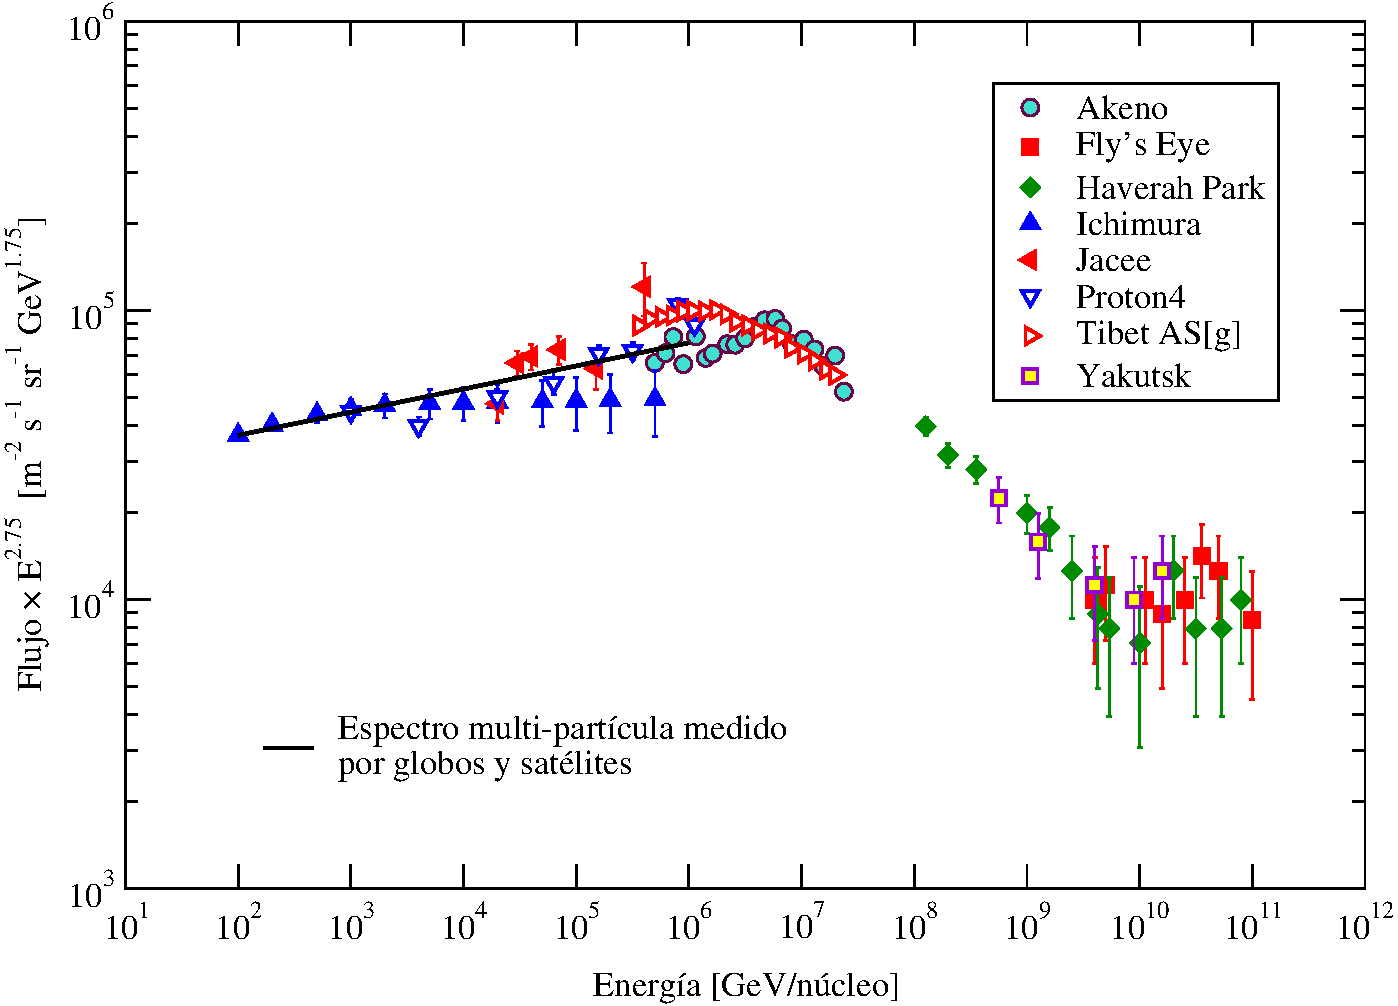
\includegraphics[width=0.75\textwidth]{CRspectrum_e}
\caption[Espectro multi-part'icula para rayos c'osmicos]{Espectro 
  multi-part'icula para rayos c'osmicos, medido por diversos
  experimentos (tomado de \cite{wiebel:thesis})} \fi
\label{fig:crspectrum}
\end{figure}
}

%%%%%%%%%%%%%%%%%%%%%%%%%%%%%%%%%%%%%%%%%%%%%%%%%%%%%%%%%%%%
\def\abundfig{
\begin{figure}[tb]
\centering
\ifenglish
\includegraphics[width=0.85\textwidth]{abund}
\caption[Abundances of the various nuclei in the cosmic 
rays]{Abundances of the various nuclei in the cosmic rays compared to
  the abundances in the Solar System: (a) Elements H -- Ni, normalized
  to $\text{Si}=1$, cosmic ray flux at $1\u{TeV/nucleus}$; (b)
  Elements Fe -- Fm, normalized to $\text{Fe}=10^6$, cosmic ray flux
  $>1.5\u{GeV/nucleon}$ (taken from \cite{wiebel:thesis})} 
\else
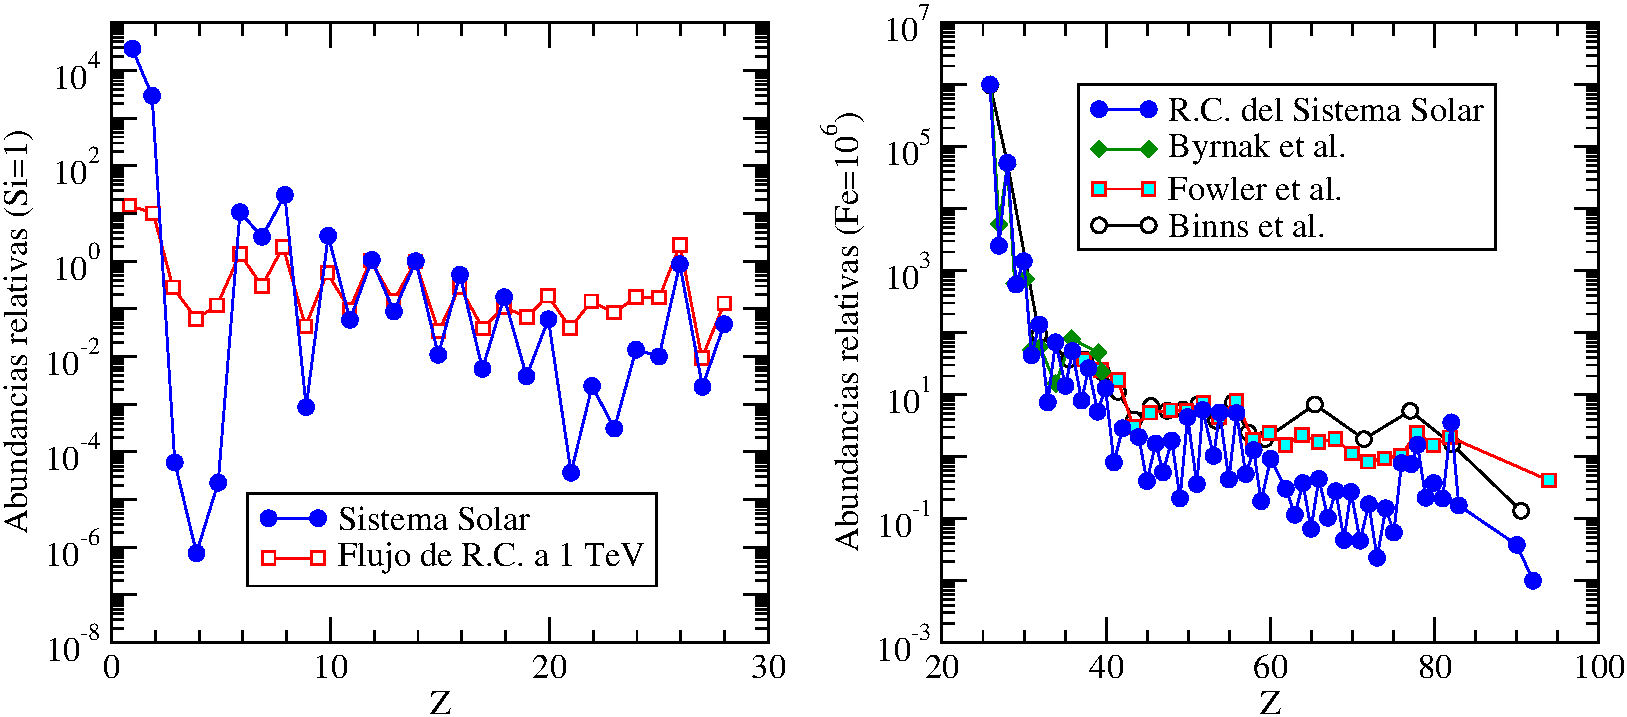
\includegraphics[width=0.85\textwidth]{abund_e}
\caption{Abundancias de los diversos n'ucleos en los rayos c{\'o}smicos, 
  comparadas con las abundancias en el Sistema Solar: (a) Elementos H
  -- Ni, normalizado a $\text{Si}=1$, flujo de rayos c{\'o}smicos a
  $1\u{TeV/\text{n{\'u}cleo}}$; (b) Elementos Fe -- Fm, normalizado a
  $\text{Fe}=10^6$, flujo de rayos c{\'o}smicos
  $>1.5\u{GeV/\text{nucle{\'o}n}}$ (tomado de \cite{wiebel:thesis})} \fi
\label{fig:abund}
\end{figure}
}

%%%%%%%%%%%%%%%%%%%%%%%%%%%%%%%%%%%%%%%%%%%%%%%%%%%%%%%%%%%%
\def\elemespectrofig{
\begin{figure}[t]
\centering
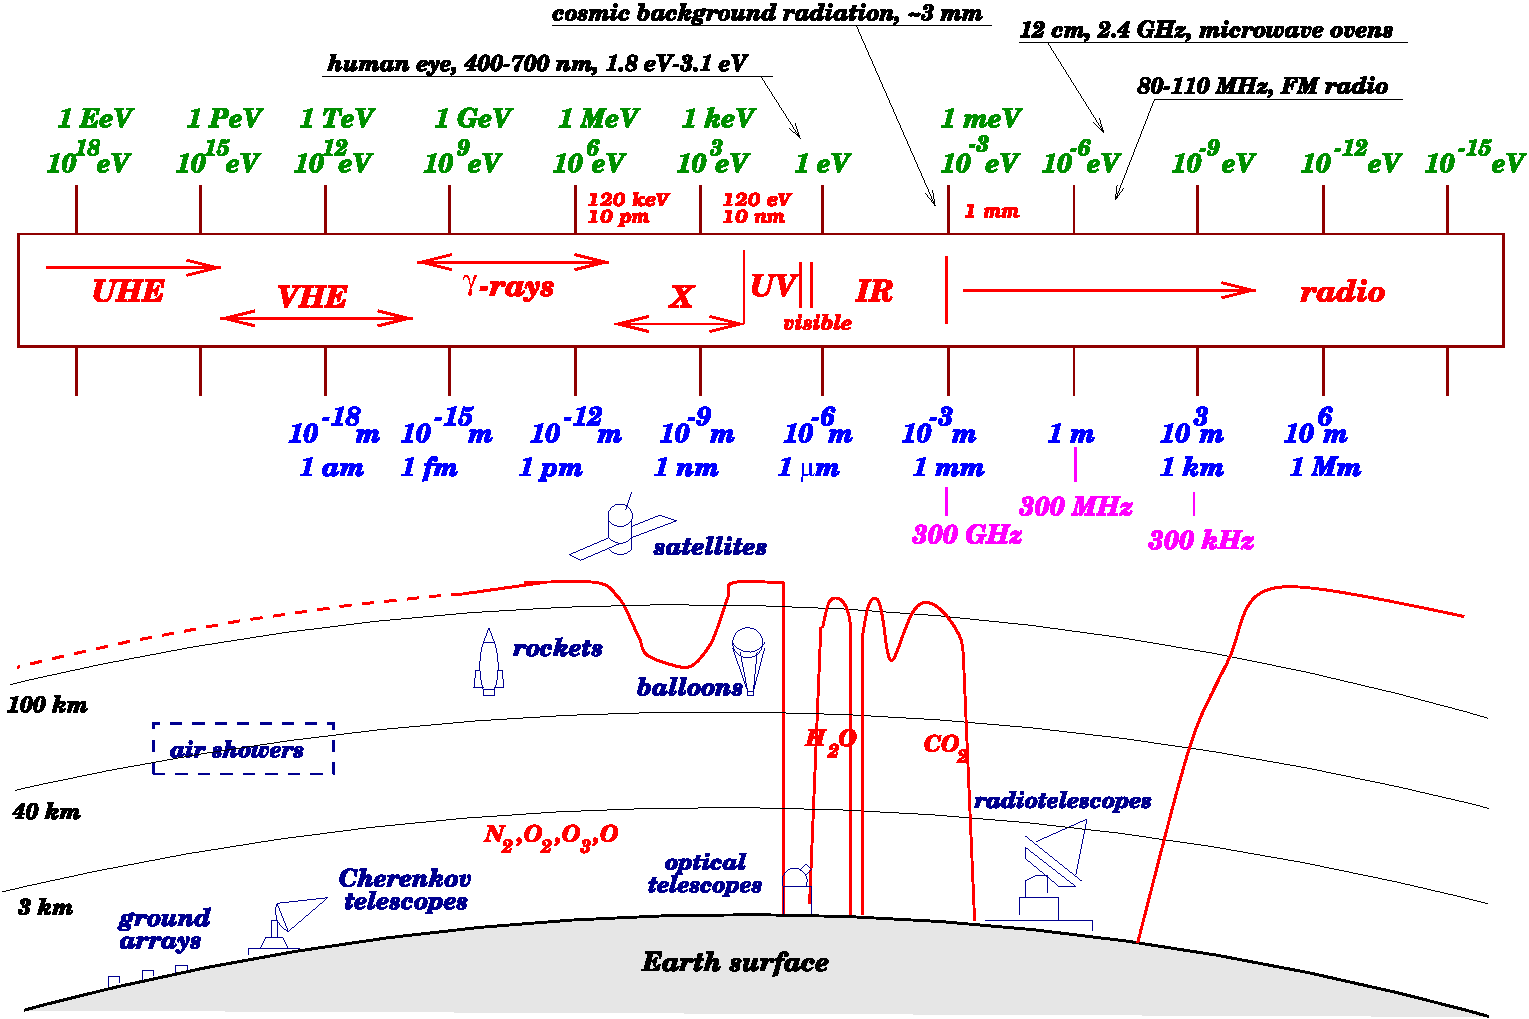
\includegraphics[width=0.95\textwidth]{espectro}
\ifenglish
\caption[The electromagnetic spectrum]{Schematic view of the whole 
  electromagnetic spectrum}
\else
\caption[El espectro electromagn'etico]{Visi'on esquem'atica
  del espectro electromagn'etico}
\fi
\label{fig:electrspec}
\end{figure}
}

%%%%%%%%%%%%%%%%%%%%%%%%%%%%%%%%%%%%%%%%%%%%%%%%%%%%%%%%%%%%
\def\gsourcesfig{
\begin{figure}[p]
\centering
\ifenglish
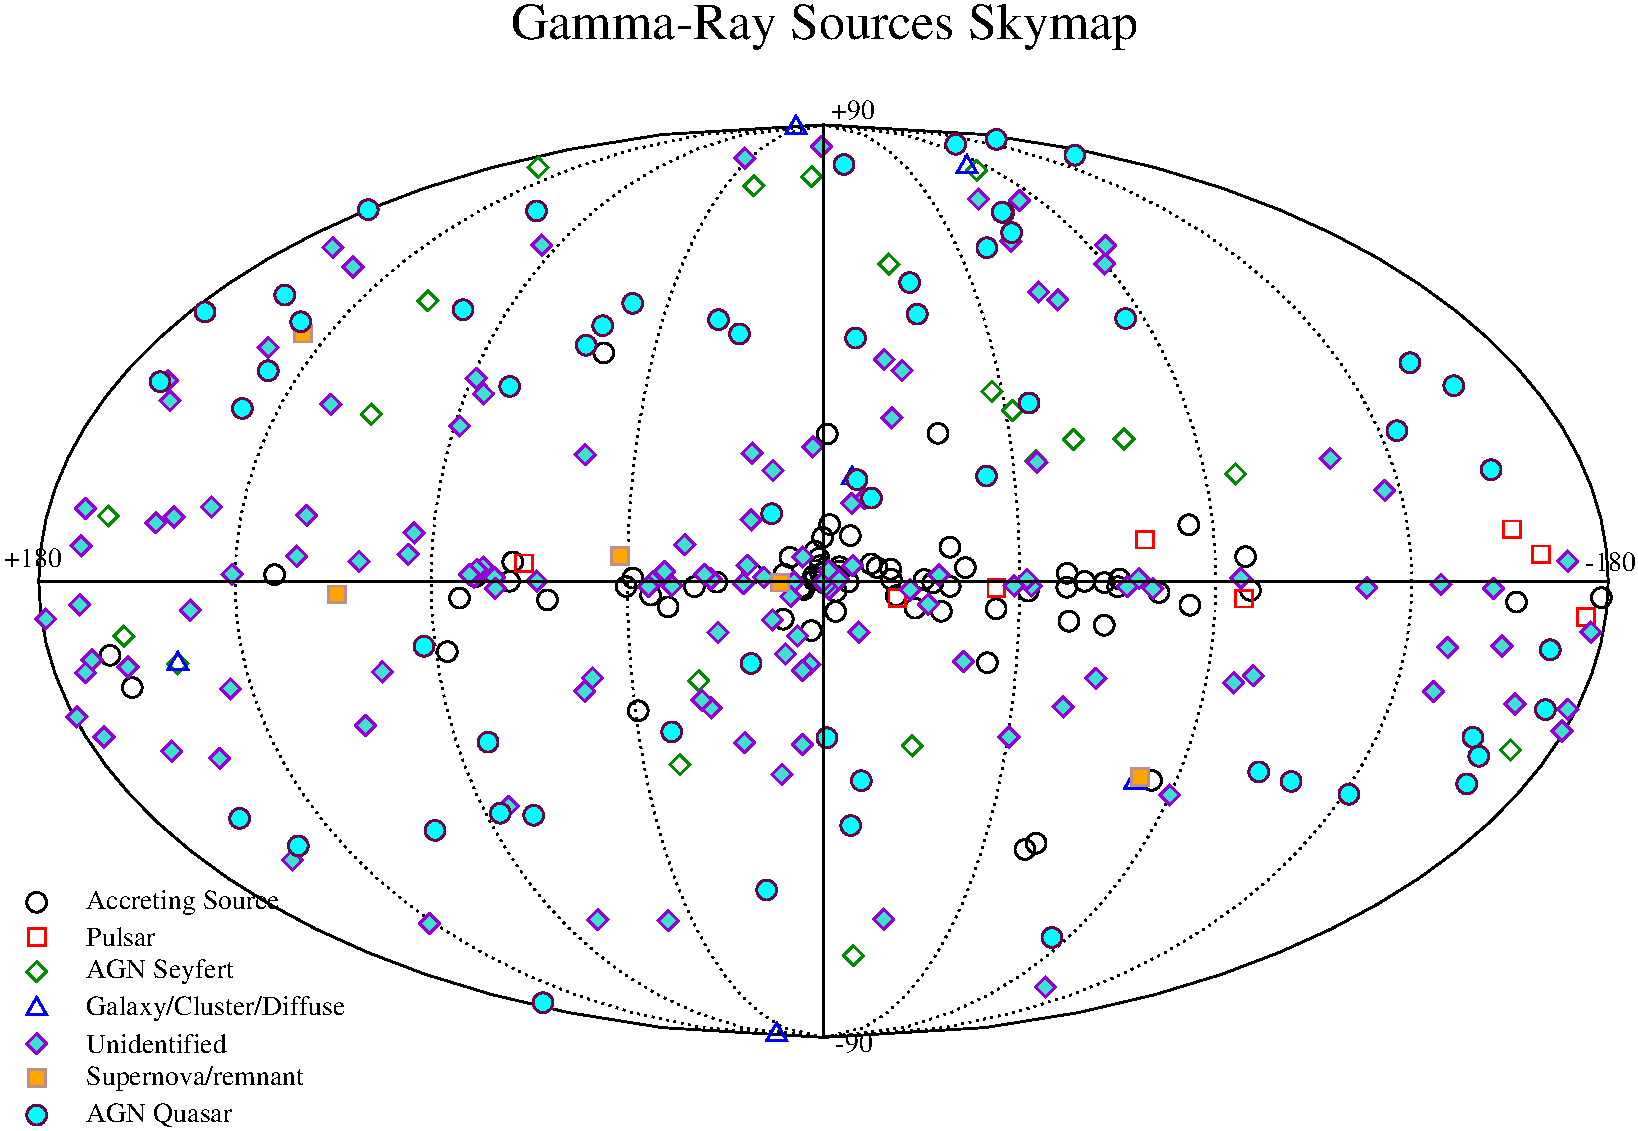
\includegraphics[width=0.95\textwidth]{gsources_bis}
\caption[A Gamma-Ray Sources Skymap]{A Gamma-Ray Sources Skymap [??].}  
\else
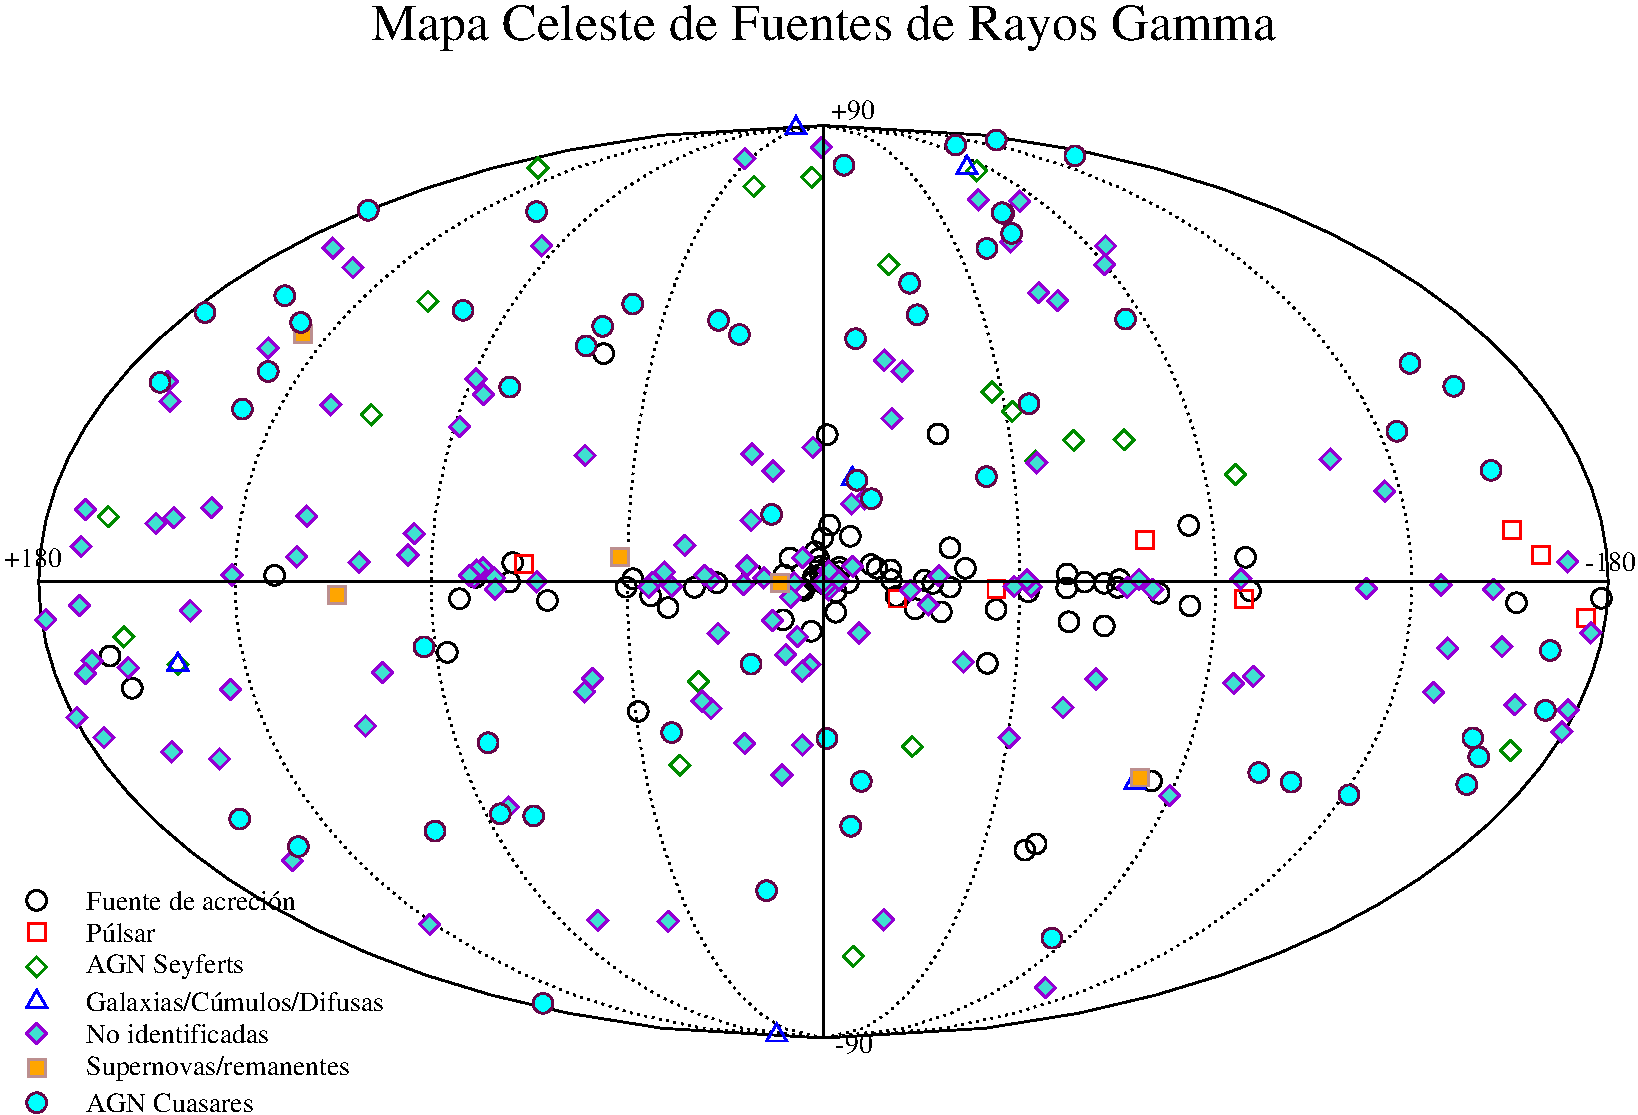
\includegraphics[width=0.95\textwidth]{gsources_bis_e}
\caption[Mapa del cielo de fuentes de rayos gamma]{Mapa del cielo de
  fuentes de rayos gamma [??].}
\fi
\label{fig:gsources}
\end{figure}
}

%%%%%%%%%%%%%%%%%%%%%%%%%%%%%%%%%%%%%%%%%%%%%%%%%%%%%%%%%%%%
\def\gsnumbersfig{
\begin{figure}[p]
\centering
\ifenglish
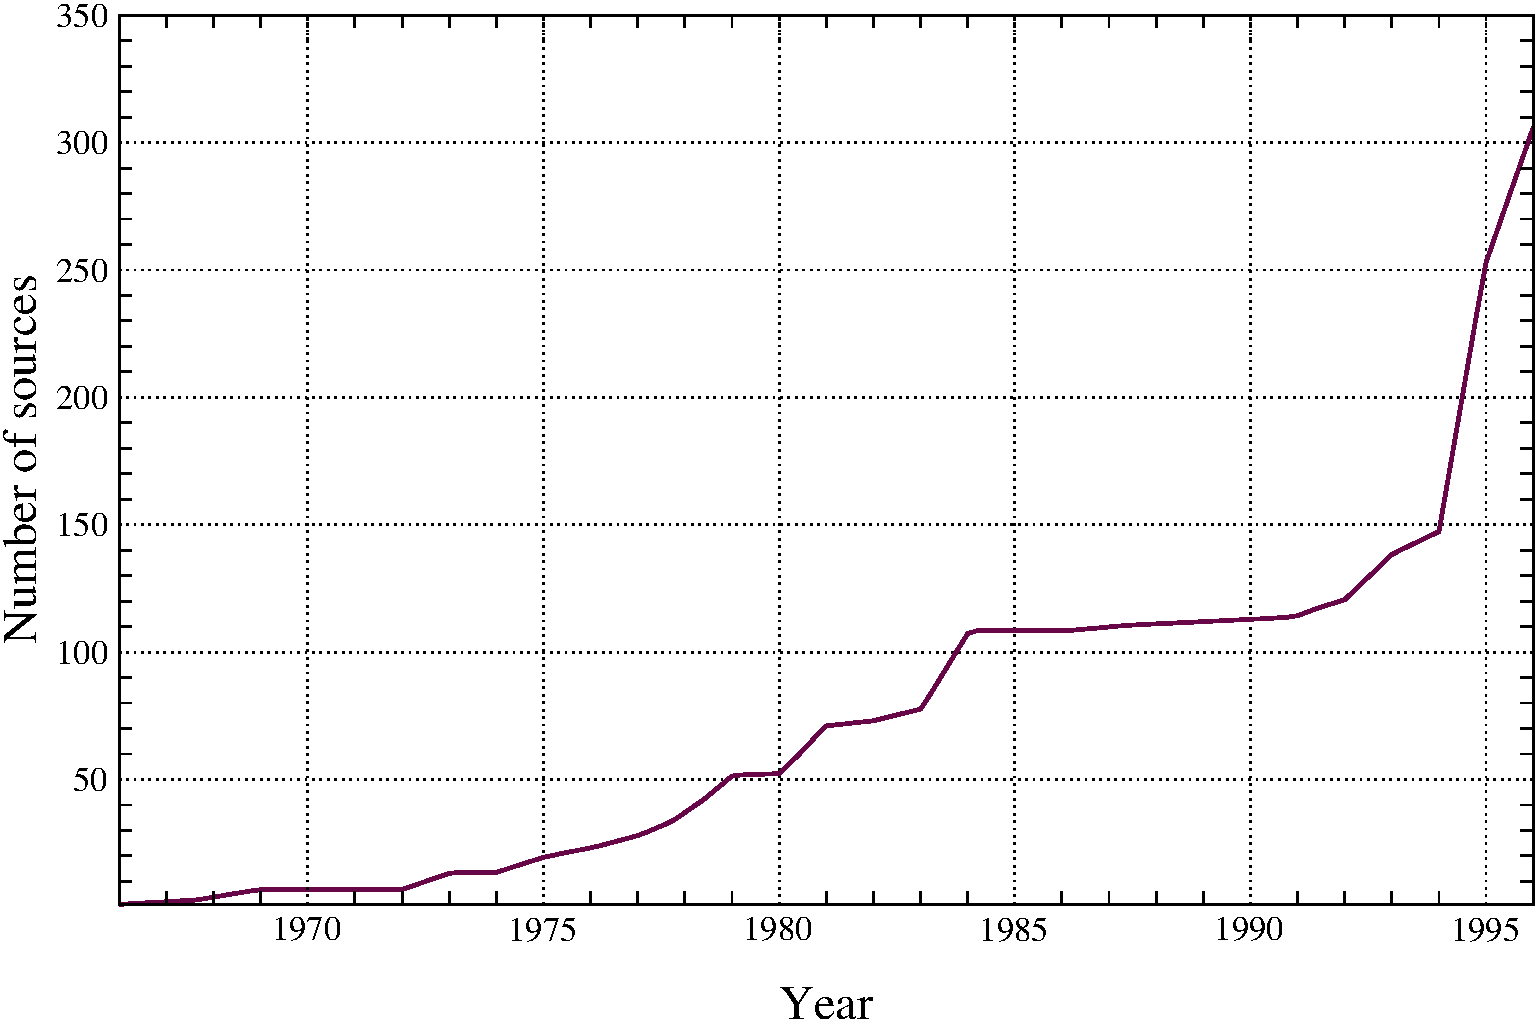
\includegraphics[width=0.65\textwidth]{gsnumbers}
\caption[Number of observed gamma-ray sources]{Number of observed
  gamma-ray sources, in the period 1966--1996. Adapted from [??].}
\else 
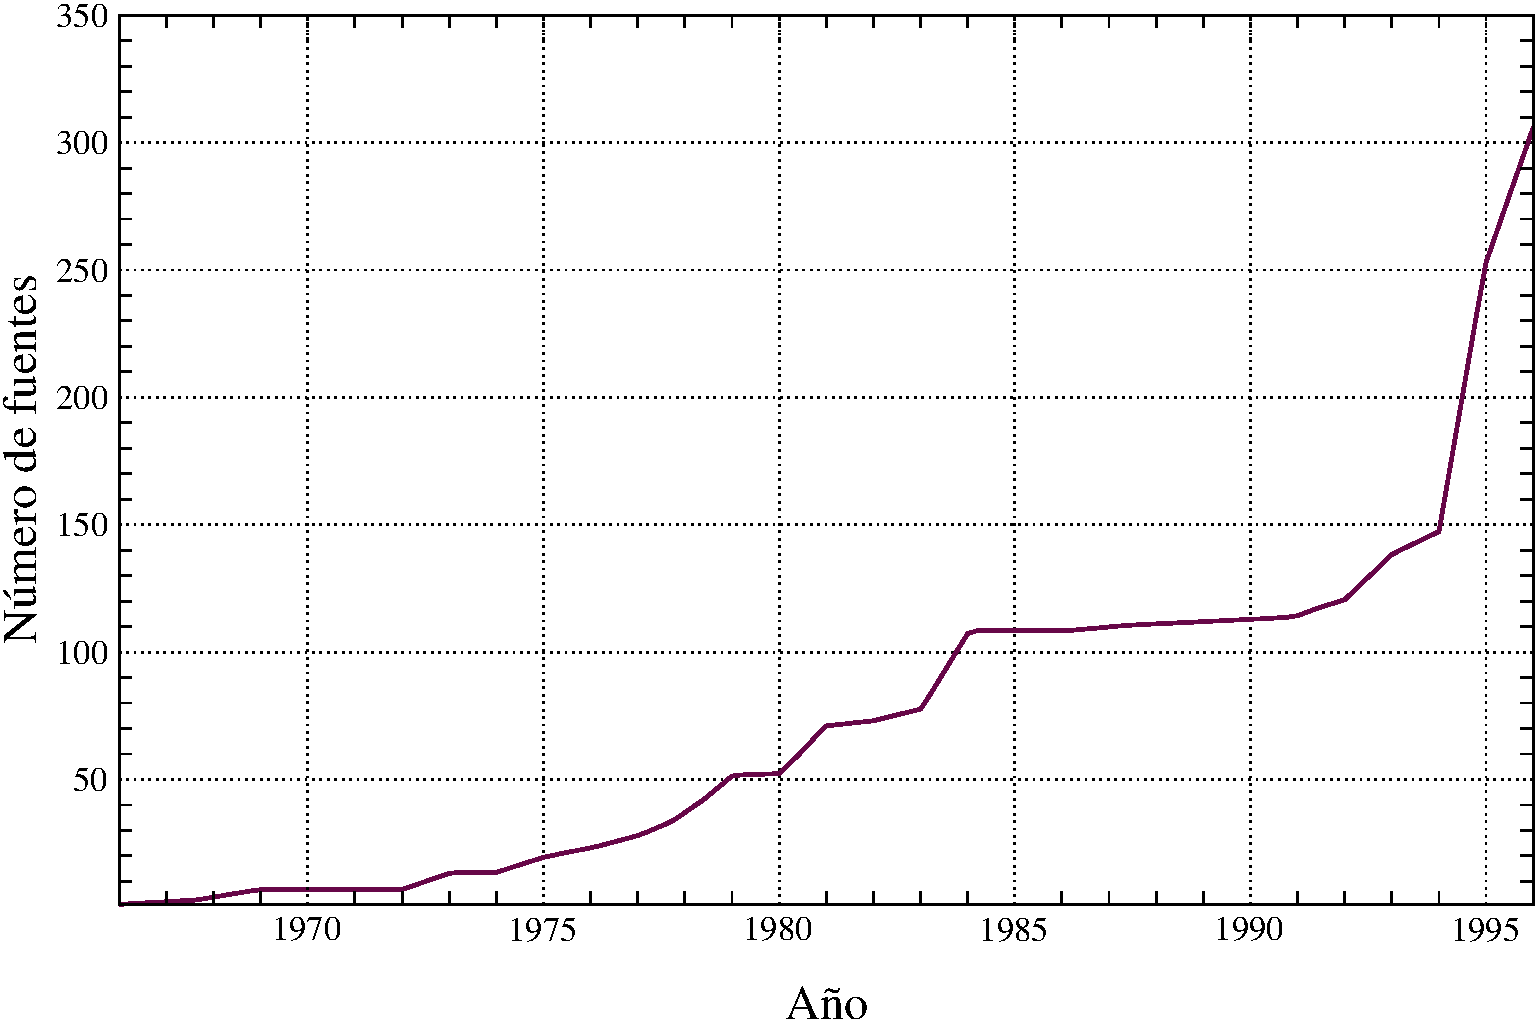
\includegraphics[width=0.65\textwidth]{gsnumbers_e}
\caption[N'umero de fuentes de rayos gamma descubiertas]{N'umero de
  fuentes de rayos gamma descubiertas, a lo largos del per'iodo
  1.966--1.996.  Adaptado de [??].}  
\fi
\label{fig:gsnumbers}
\end{figure}
}

%%%%%%%%%%%%%%%%%%%%%%%%%%%%%%%%%%%%%%%%%%%%%%%%%%%%%%%%%%%%
\def\pulsarschfig{
%\begin{figure}[p]
\begin{wrapfigure}[21]{r}{0.44\textwidth}
\centering
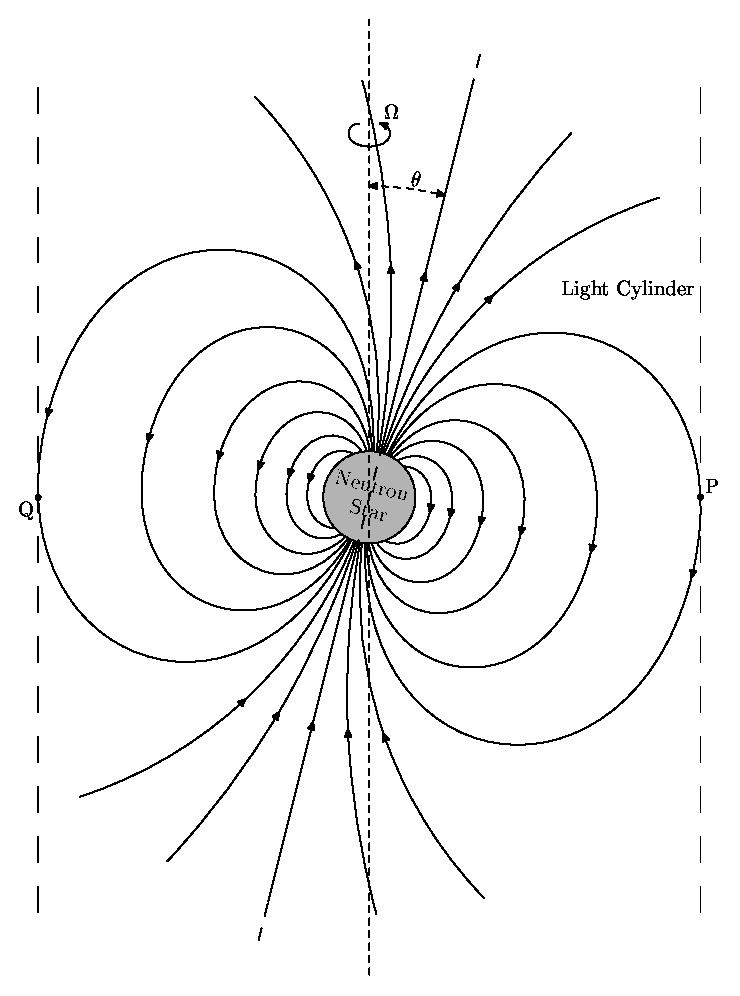
\includegraphics[width=0.43\textwidth]{pulsar}
\ifenglish
\caption{Schematic model of a pulsar}
\else
\caption{Visi'on esquem'atica de un p'ulsar}
\fi
\label{fig:pulsarsch}
\end{wrapfigure}
%\end{figure}
}

%%%%%%%%%%%%%%%%%%%%%%%%%%%%%%%%%%%%%%%%%%%%%%%%%%%%%%%%%%%%
\def\bhstarevolfig{
\begin{figure}[p]
\centering
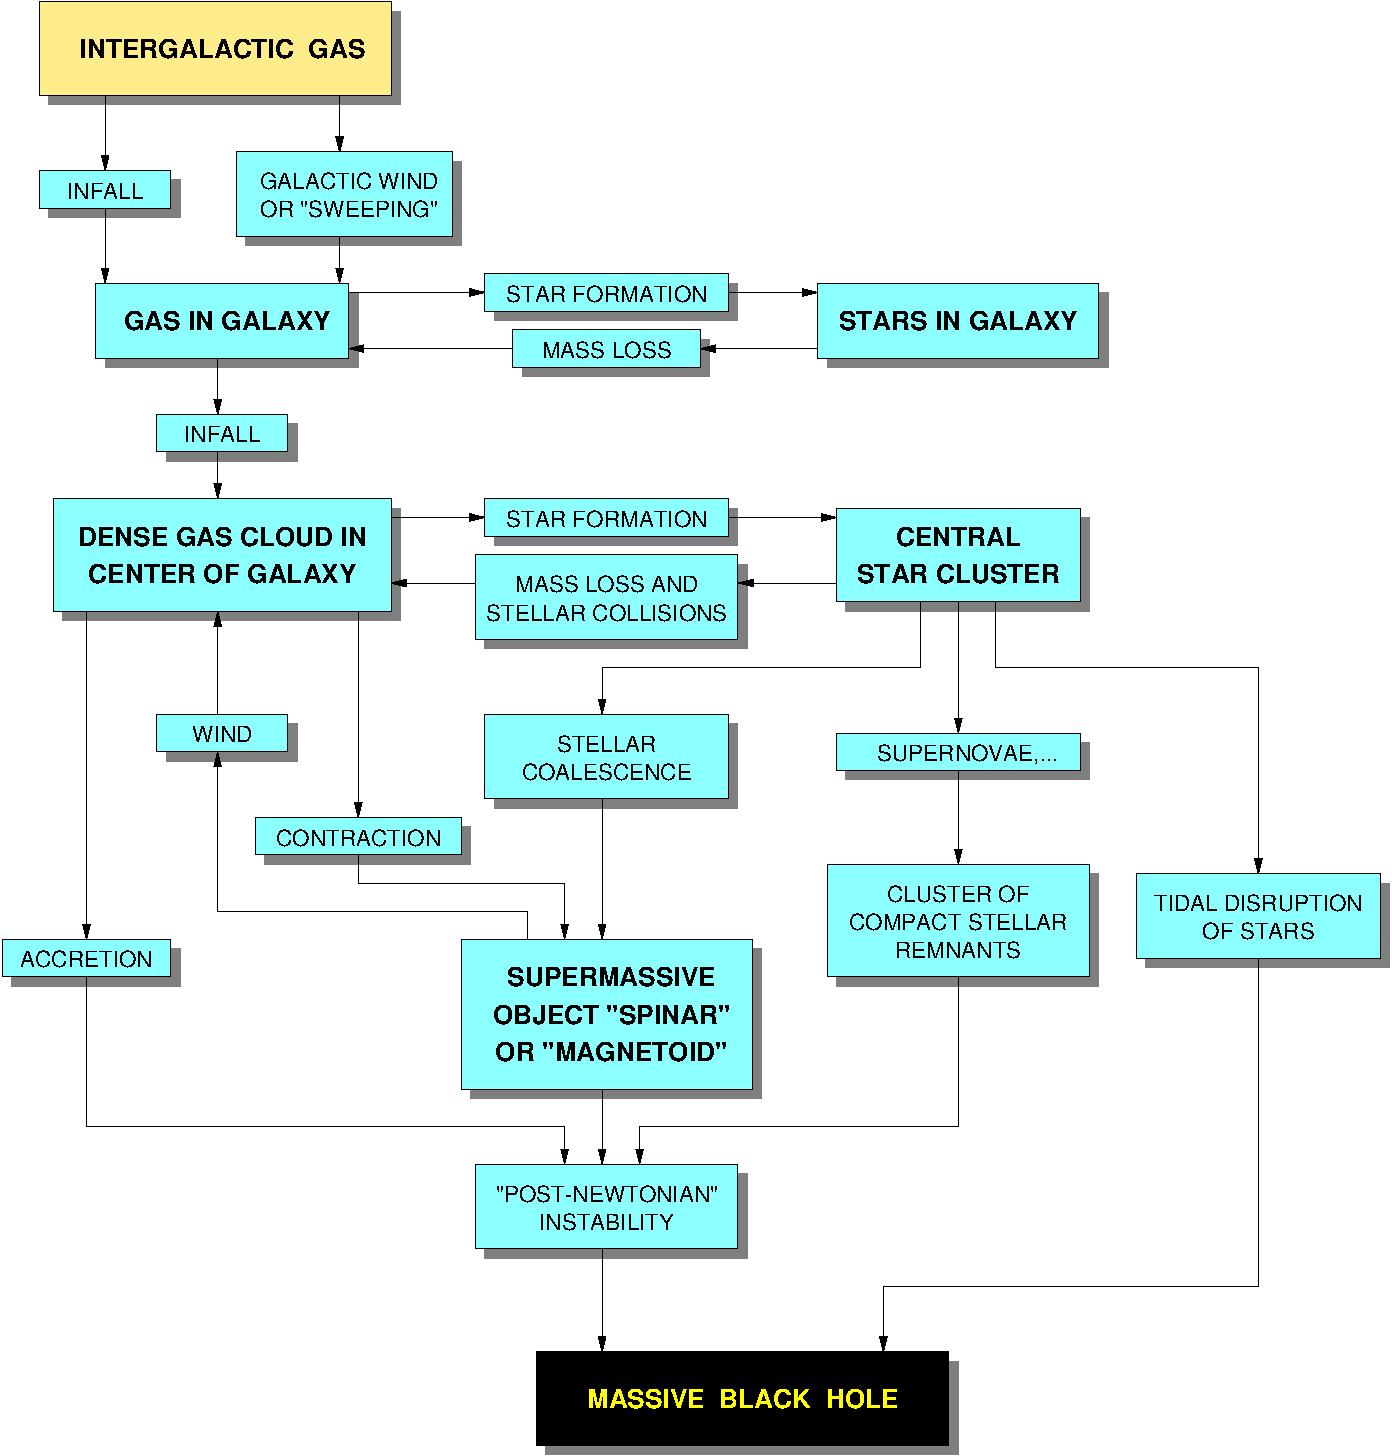
\includegraphics[width=0.95\textwidth]{bhstarevol}
\ifenglish
\caption[Possible evoutionary sequence for massive gas
clouds]{Schematic representation of the possible evoutionary sequence
  for massive gas clouds. Almost all tracks lead to the black hole
  state (take from \cite{BarrowTipler:Antrop})}
\else
\caption[Posible secuencia evolutiva de nubes de gas
masivas]{Representaci'on esquem'atica de la posible secuencia
  evolutiva de nubes de gas masivas. Casi todos los caminos llevan al
  estado de agujero negro (tomado de \cite{BarrowTipler:Antrop})} 
\fi
\label{fig:bhstarevol}
\end{figure}
}

%%%%%%%%%%%%%%%%%%%%%%%%%%%%%%%%%%%%%%%%%%%%%%%%%%%%%%%%%%%%
%% ATMOPHERIC GAMMA AND COSMIC RAY SHOWERS %%%%%%%%%%%%%%%%%
%%%%%%%%%%%%%%%%%%%%%%%%%%%%%%%%%%%%%%%%%%%%%%%%%%%%%%%%%%%%

%%%%%%%%%%%%%%%%%%%%%%%%%%%%%%%%%%%%%%%%%%%%%%%%%%%%%%%%%%%%
\def\atmshowerfig{
\begin{figure}
\centering
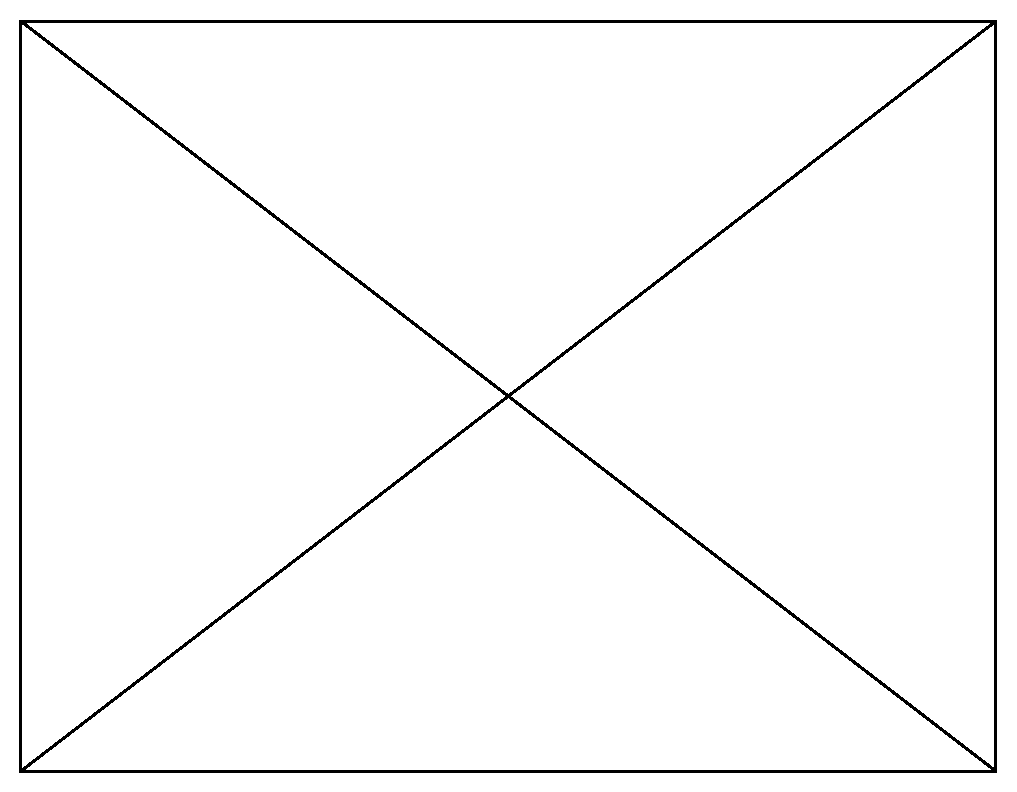
\includegraphics[height=0.8\textheight,width=0.9\textwidth]{dummy-figure}
\ifenglish
\caption[Artistic view of an atmospheric shower.]{Artistic view of the 
  generation of an atmospheric shower. Notice that in this
  representation a complete interval of time (and not only an instant)
  is taken into account, since the shower, actually, doesn't exist as
  a whole in any moment, but evolves from the top part of the
  atmosphere until the maximum of development, and from this point to
  the ground (or even below the observation level, inside the Earth)}
\else   
\caption[Visi'on art'istica de una cascada atmosf'erica.]{Visi'on
  art'istica del desarrollo de una cascada atmosf'erica.  N'otese que
  en esta representaci'on un cierto intervalo de tiempo (el que tarda
  la cascada en generarse) ha sido tenido en cuenta, y no un simple
  instante temporal. Esto es as'i porque, evidentemente, la cascada no
  existe en ning'un instante determinado como un todo, sino que
  evoluciona desde su inicio en la zona superior de la atm'osfera
  hasta su m'aximo desarrollo, y desde este punto hasta el nivel de
  observaci'on (e incluso por debajo, en el interior de la tierra)}
\fi
\label{fig:atmshower}
\end{figure}
}

%%%%%%%%%%%%%%%%%%%%%%%%%%%%%%%%%%%%%%%%%%%%%%%%%%%%%%%%%%%%
\def\processesfig{
\begin{figure}[t]
\centering
\ifenglish
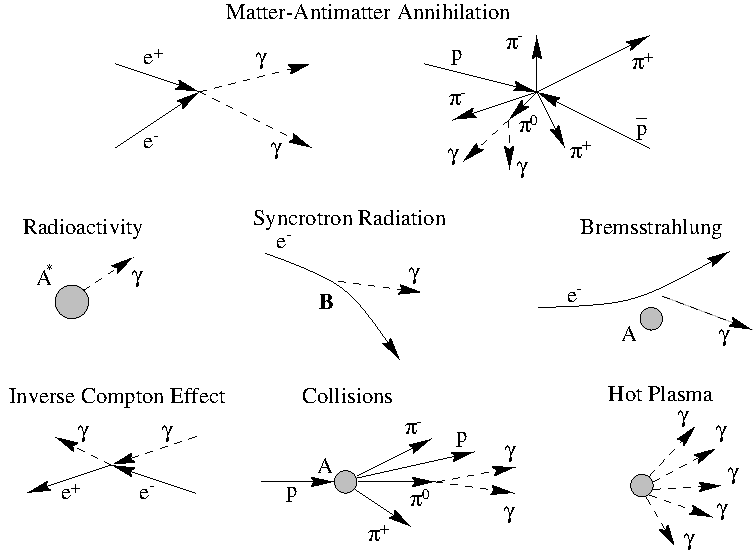
\includegraphics[width=0.7\textwidth]{processes}
\caption{Physical processes related to the generation of gamma rays}
\else
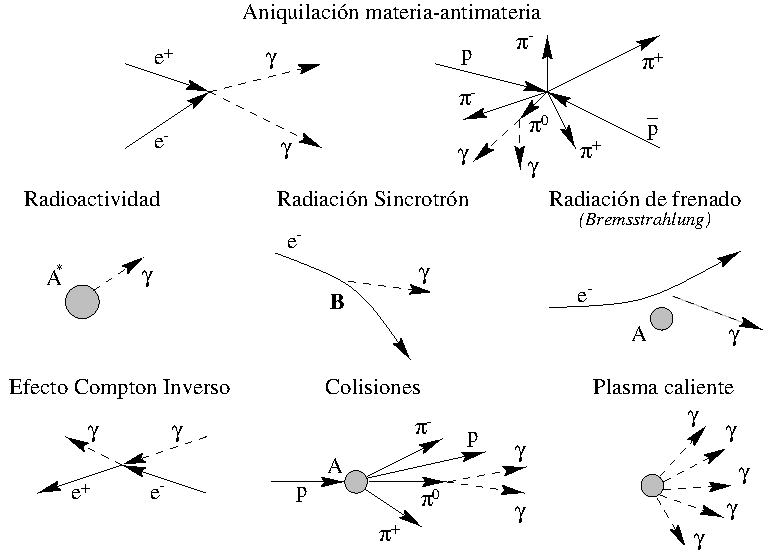
\includegraphics[width=0.7\textwidth]{processes_e}
\caption{Procesos f'isicos implicados en la generaci'on de rayos gamma}
\fi
\label{fig:processes}
\end{figure}
}

%%%%%%%%%%%%%%%%%%%%%%%%%%%%%%%%%%%%%%%%%%%%%%%%%%%%%%%%%%%%
\def\toymodelfig{
\begin{wrapfigure}{r}{.3\textwidth}
%\begin{narrow}{0cm}{-1cm}
\ifenglish
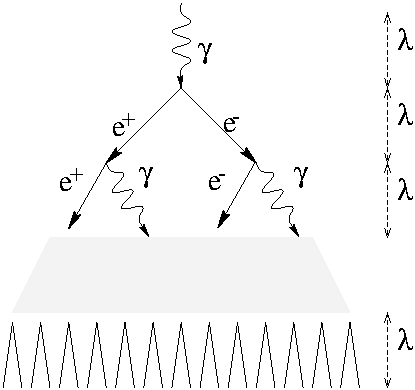
\includegraphics[width=.3\textwidth]{toymodel}
\caption[Scheme of the development of an electromagnetic
  atmospheric shower (\emph{toy-model})]{Schematized view of the
  development of an electromagnetic atmospheric shower
  (\emph{toy-model})} 
\else
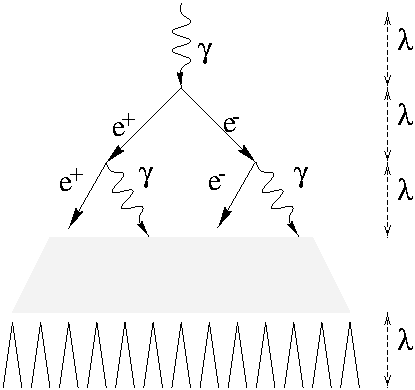
\includegraphics[width=.3\textwidth]{toymodel_e}
\caption{Visi'on esquem'atica del desarrollo de una cascada 
  electromagn'etica (\emph{modelo de jugete})} 
\fi
\label{fig:toymodel}
%\end{narrow}
\end{wrapfigure}
}

%%%%%%%%%%%%%%%%%%%%%%%%%%%%%%%%%%%%%%%%%%%%%%%%%%%%%%%%%%%%
\def\hadronicfig{
\begin{figure}[tbh]
%\begin{wrapfigure}{l}{0.5\textwidth}
\centering
\ifenglish
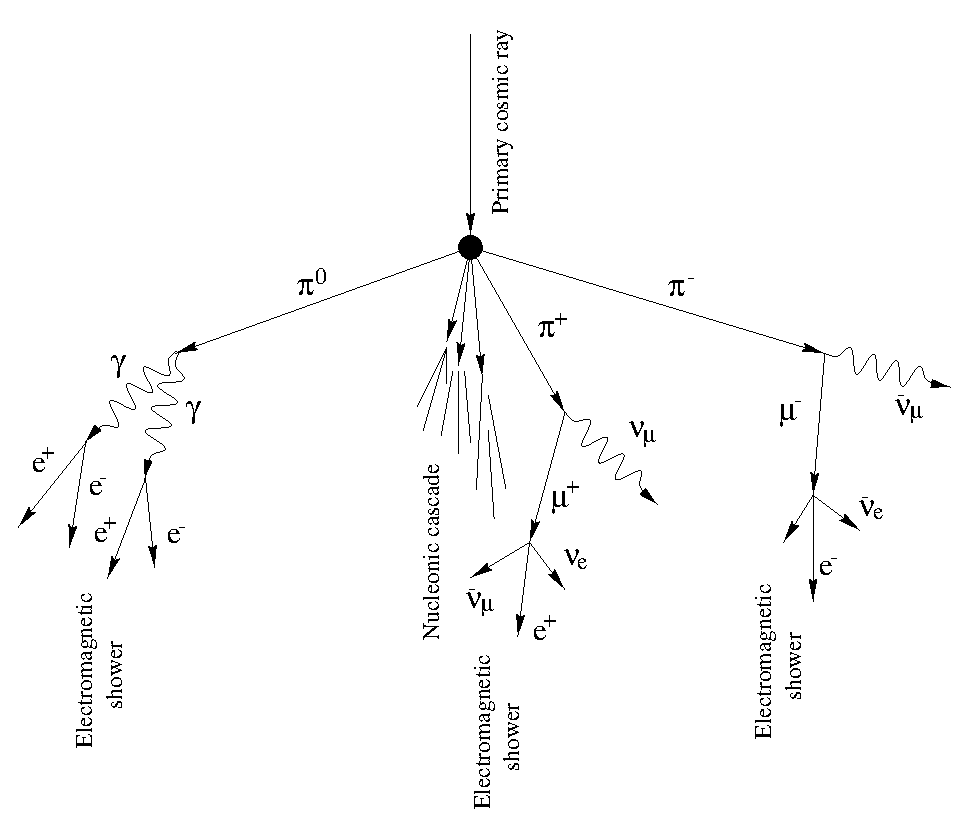
\includegraphics[width=0.5\textwidth]{hadronic}
\caption[A schematic diagram of the development of a hadronic cascade
  in the atmosphere]{A schematic diagram of the development of a
  hadronic cascade in the atmosphere (adapted from
  \cite{Sokolsky:book})}
\else
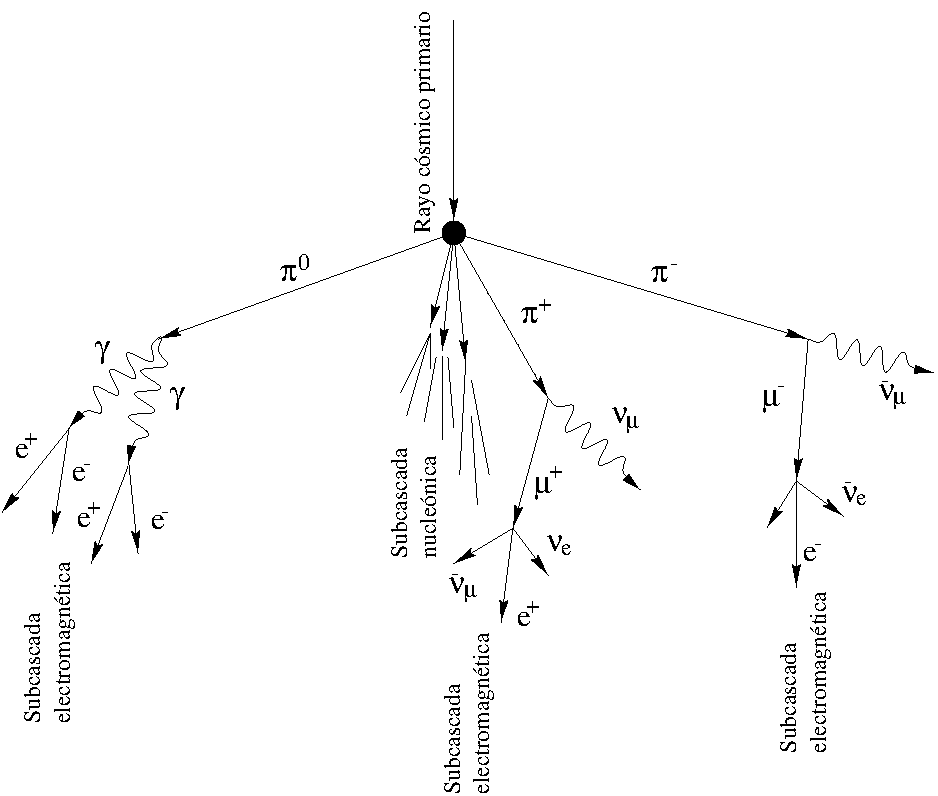
\includegraphics[width=0.5\textwidth]{hadronic_e}
\caption[Diagrama esquem'atico del desarrollo de una cascada 
  hadr'onica]{Diagr'ama esquem'atico del desarrollo de una cascada
  hadr'onica en la atm'osfera (adaptado de \cite{Sokolsky:book})}
\fi
\label{fig:hadronic}
%\end{wrapfigure}
\end{figure}
}

%%%%%%%%%%%%%%%%%%%%%%%%%%%%%%%%%%%%%%%%%%%%%%%%%%%%%%%%%%%%%
%\def\lognefig{
%\begin{figure}[p]
%\centering
%\ifenglish
%\includegraphics[width=0.65\textwidth]{longdistteo}
%\caption[Longitudinal development of an electromagnetic atmospheric
%shower]{Theoretical longitudinal development of an electromagnetic
%  atmospheric shower. The numbers in blue (6 to 26) correspond to
%  different values of $x=\ln(E_0/E_{\mathrm{c}})$. The numbers
%  enclosed in red squares (0.4 to 1.8) correspond to values with
%  constant age $s$} \else
%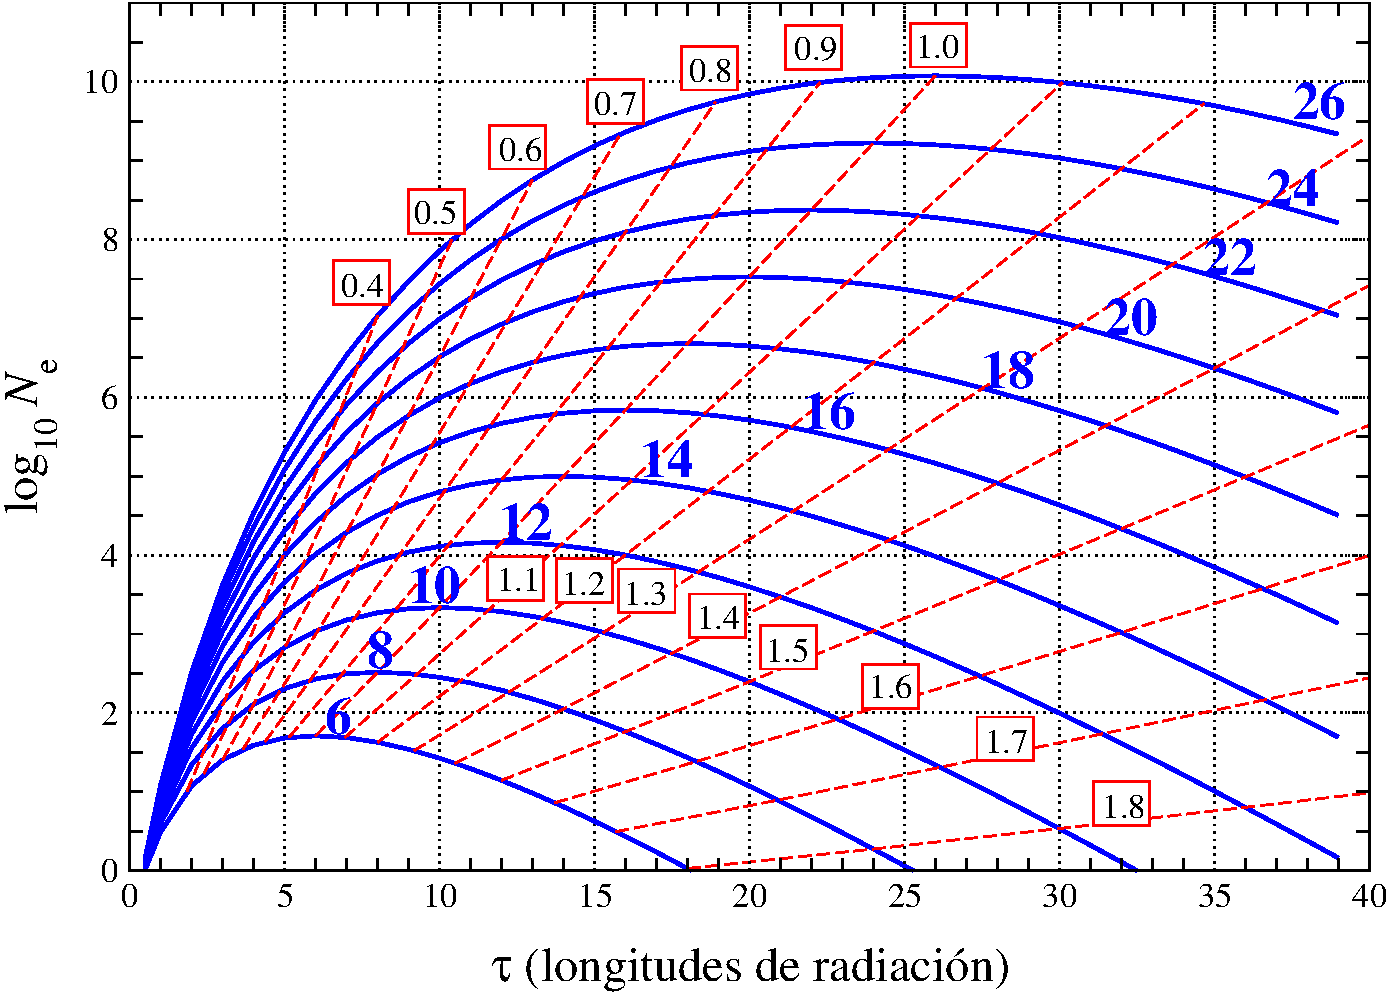
\includegraphics[width=0.65\textwidth]{longdistteo_e}
%\caption[Desarrollo longitudinal de una cascada electromagn'etica]
%{Desarrollo longitudinal te'orico de una cascada atmosf'erica
%  electromagn'etica. Los n'umeros en azul (6 a 26) corresponden a
%  diferentes valores de $x=\ln(E_0/E_{\mathrm{c}})$.  The n'umeros en
%  recuadros rojos (0.4 a 1.8) corresponden a valores con parametro de
%  edad $s$ constante} \fi
%\label{fig:logne}
%\end{figure}
%}

%%%%%%%%%%%%%%%%%%%%%%%%%%%%%%%%%%%%%%%%%%%%%%%%%%%%%%%%%%%%
\def\lognefig{
\begin{figure}[p]
\centering
\begin{minipage}[c]{.60\textwidth}
\centering
\ifenglish
\includegraphics[width=0.99\textwidth]{longdistteo}
\else
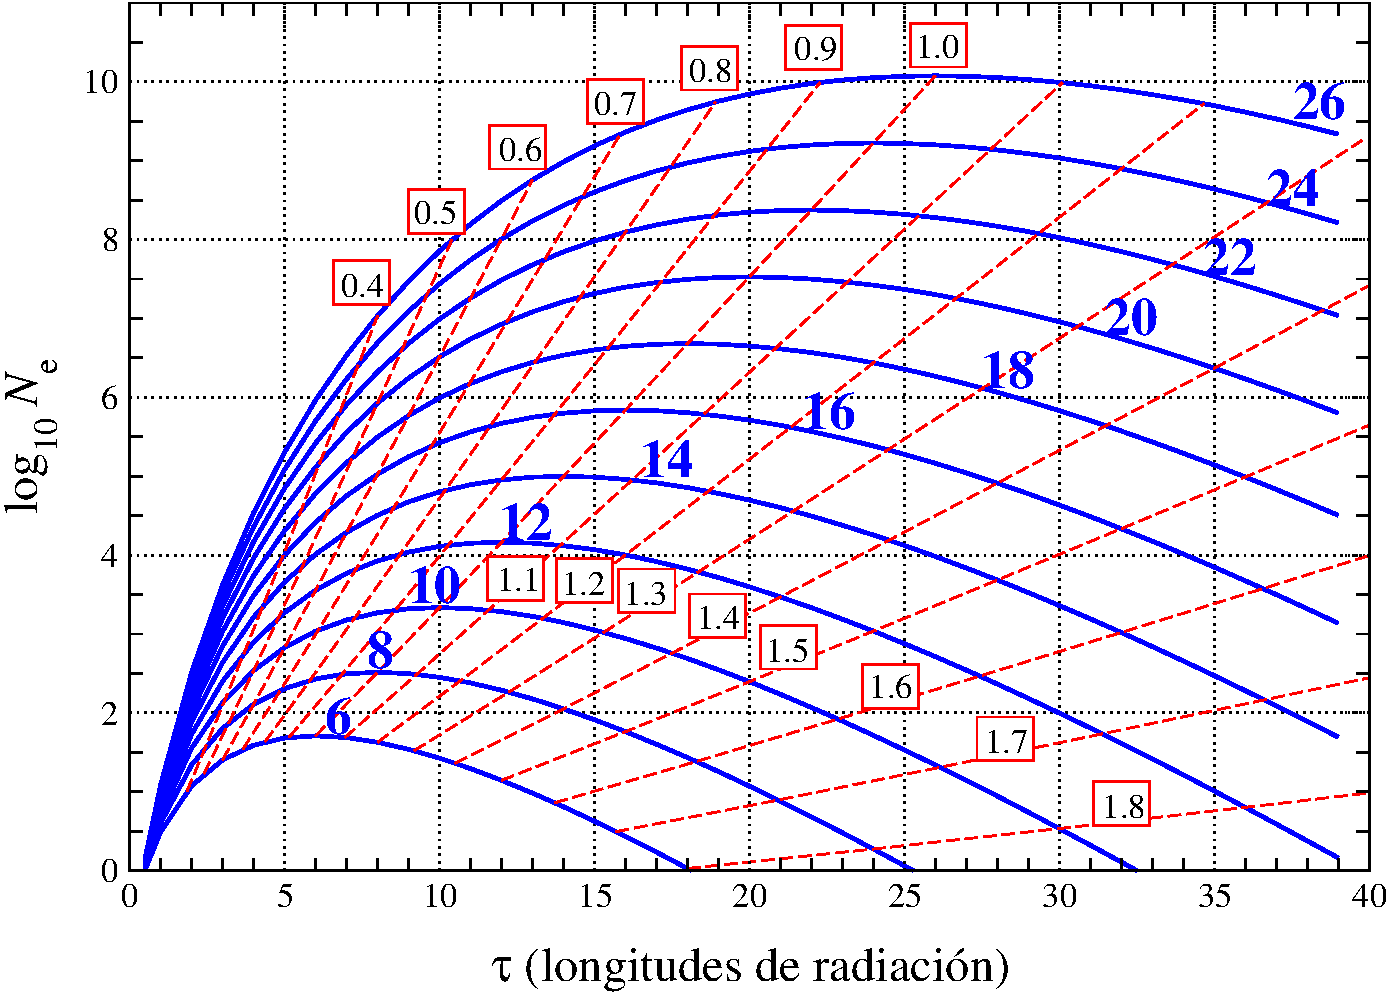
\includegraphics[width=0.99\textwidth]{longdistteo_e}
\fi
\end{minipage}
\hfill
\begin{minipage}[c]{.39\textwidth}
\centering
\ifenglish
\caption[Longitudinal development of an electromagnetic atmospheric
shower]{Theoretical longitudinal development of an electromagnetic
  atmospheric shower. The numbers in blue (6 to 26) correspond to
  different values of $x=\ln(E_0/E_{\mathrm{c}})$. The numbers
  enclosed in red squares (0.4 to 1.8) correspond to values with
  constant age $s$} \else
\caption[Desarrollo longitudinal de una cascada electromagn'etica]
{Desarrollo longitudinal te'orico de una cascada atmosf'erica
  electromagn'etica. Los n'umeros en azul (6 a 26) corresponden a
  diferentes valores de $x=\ln(E_0/E_{\mathrm{c}})$.  The n'umeros en
  recuadros rojos (0.4 a 1.8) corresponden a valores con parametro de
  edad $s$ constante} \fi
\label{fig:logne}
\end{minipage}
\end{figure}
}

%%%%%%%%%%%%%%%%%%%%%%%%%%%%%%%%%%%%%%%%%%%%%%%%%%%%%%%%%%%%
\def\samplelonglatdistfig{
\begin{figure}[p]
\centering
\hfill
\hfill
\ifenglish
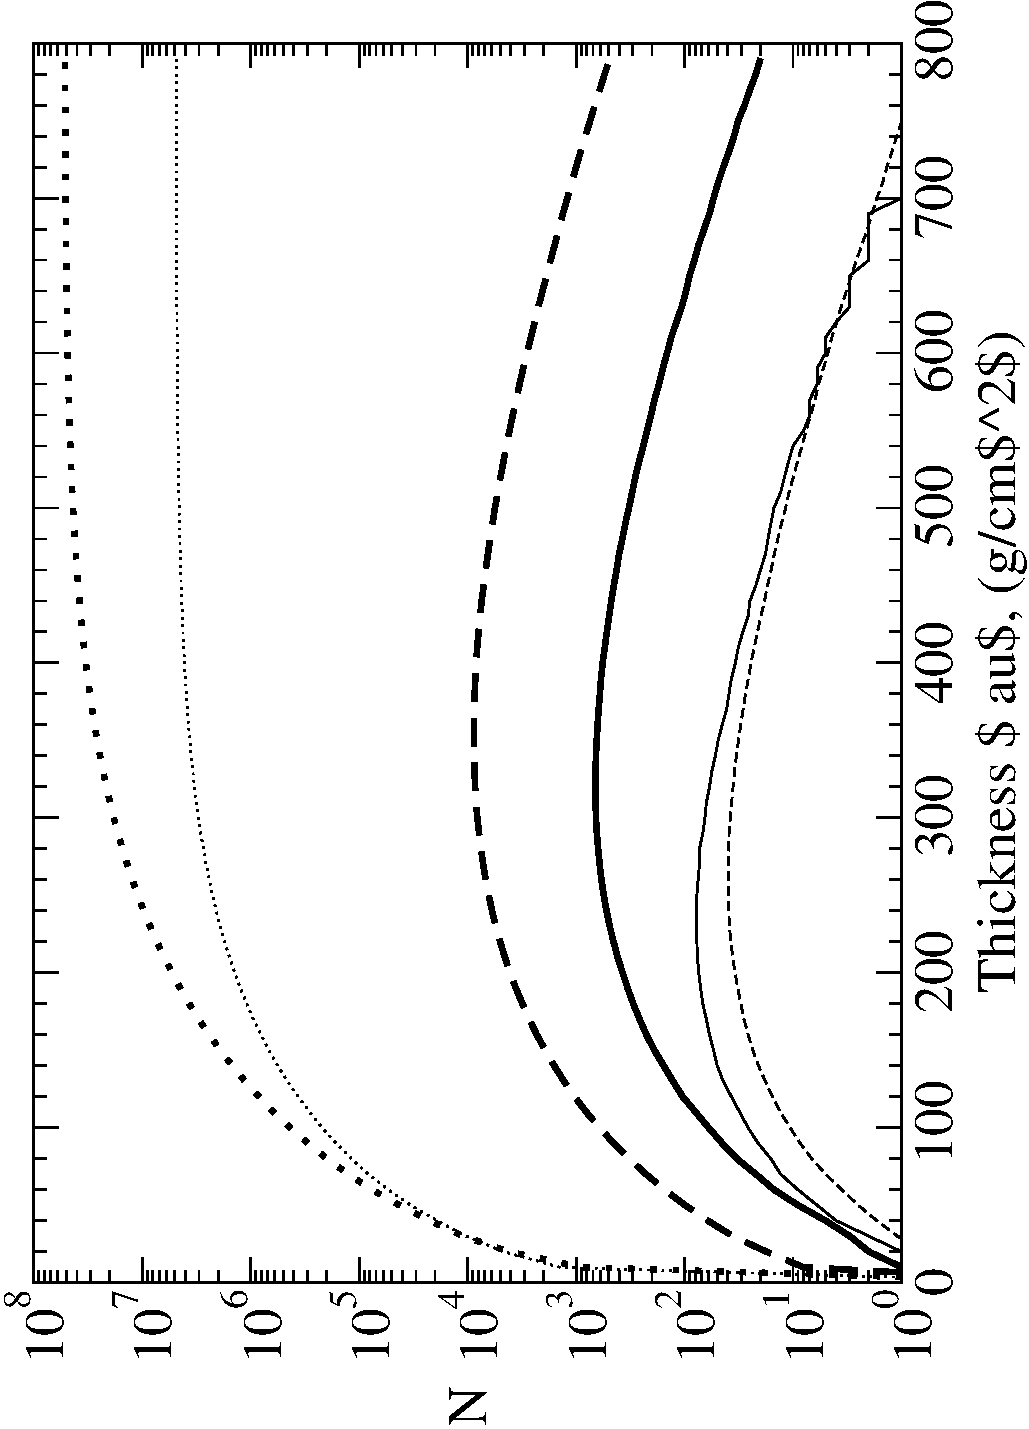
\includegraphics[width=0.35\textwidth,angle=-90,clip]{longdist_100gev-1tev}
\hfill
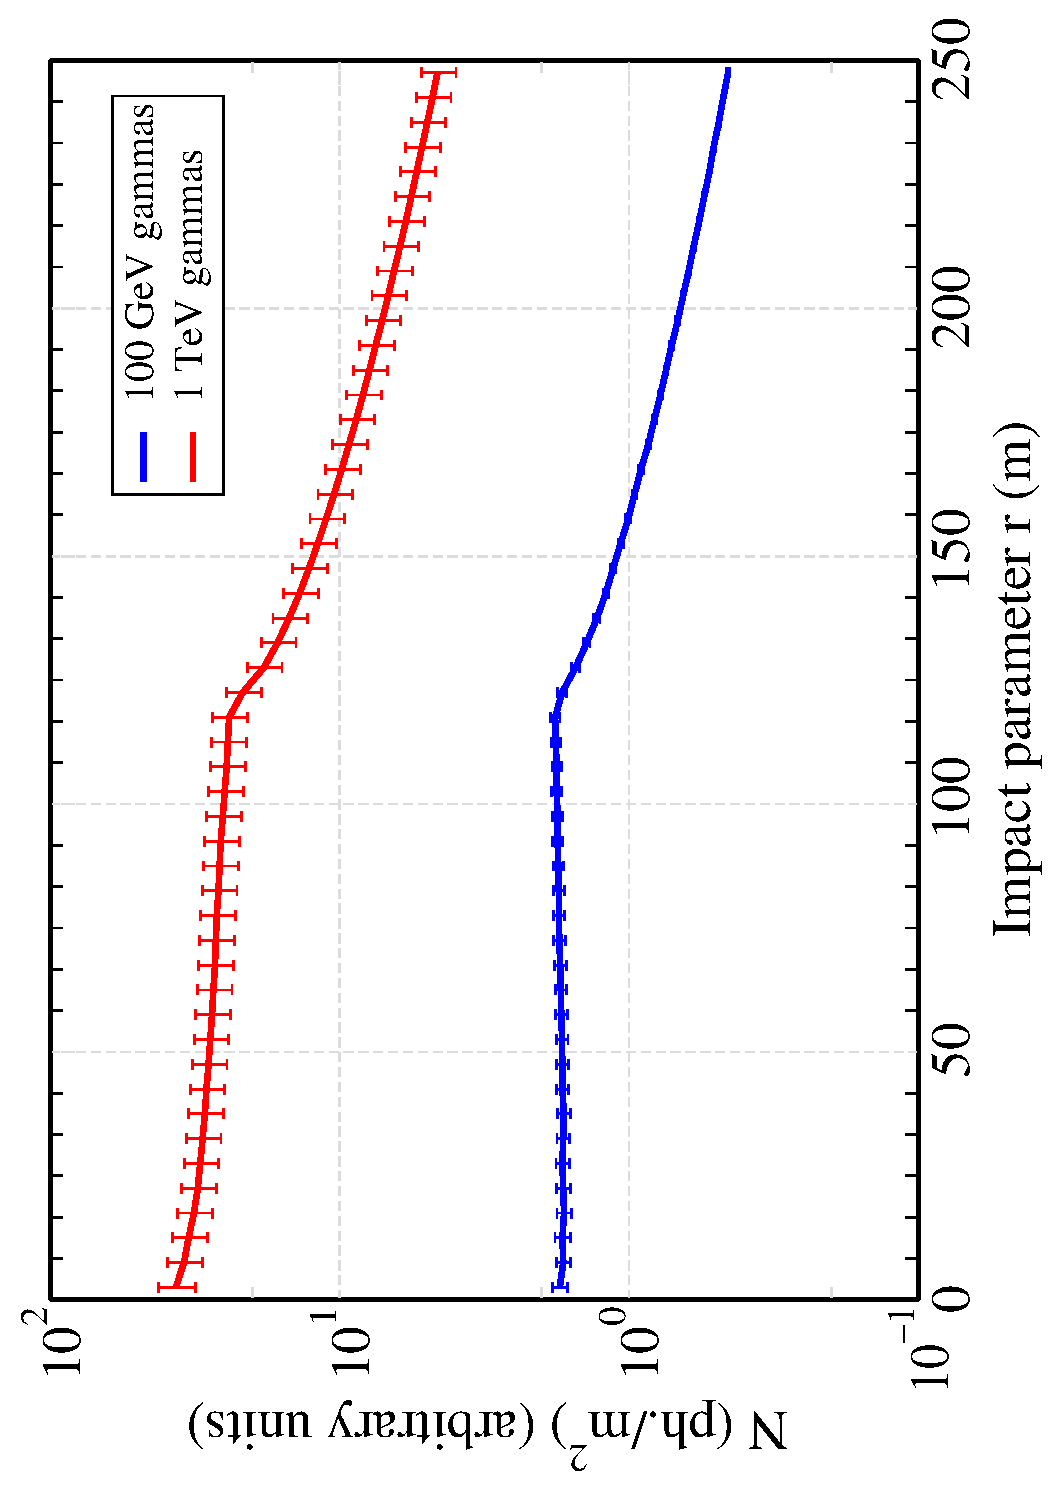
\includegraphics[width=0.35\textwidth,angle=-90,clip]{latdist_100gev-1tev}
\else
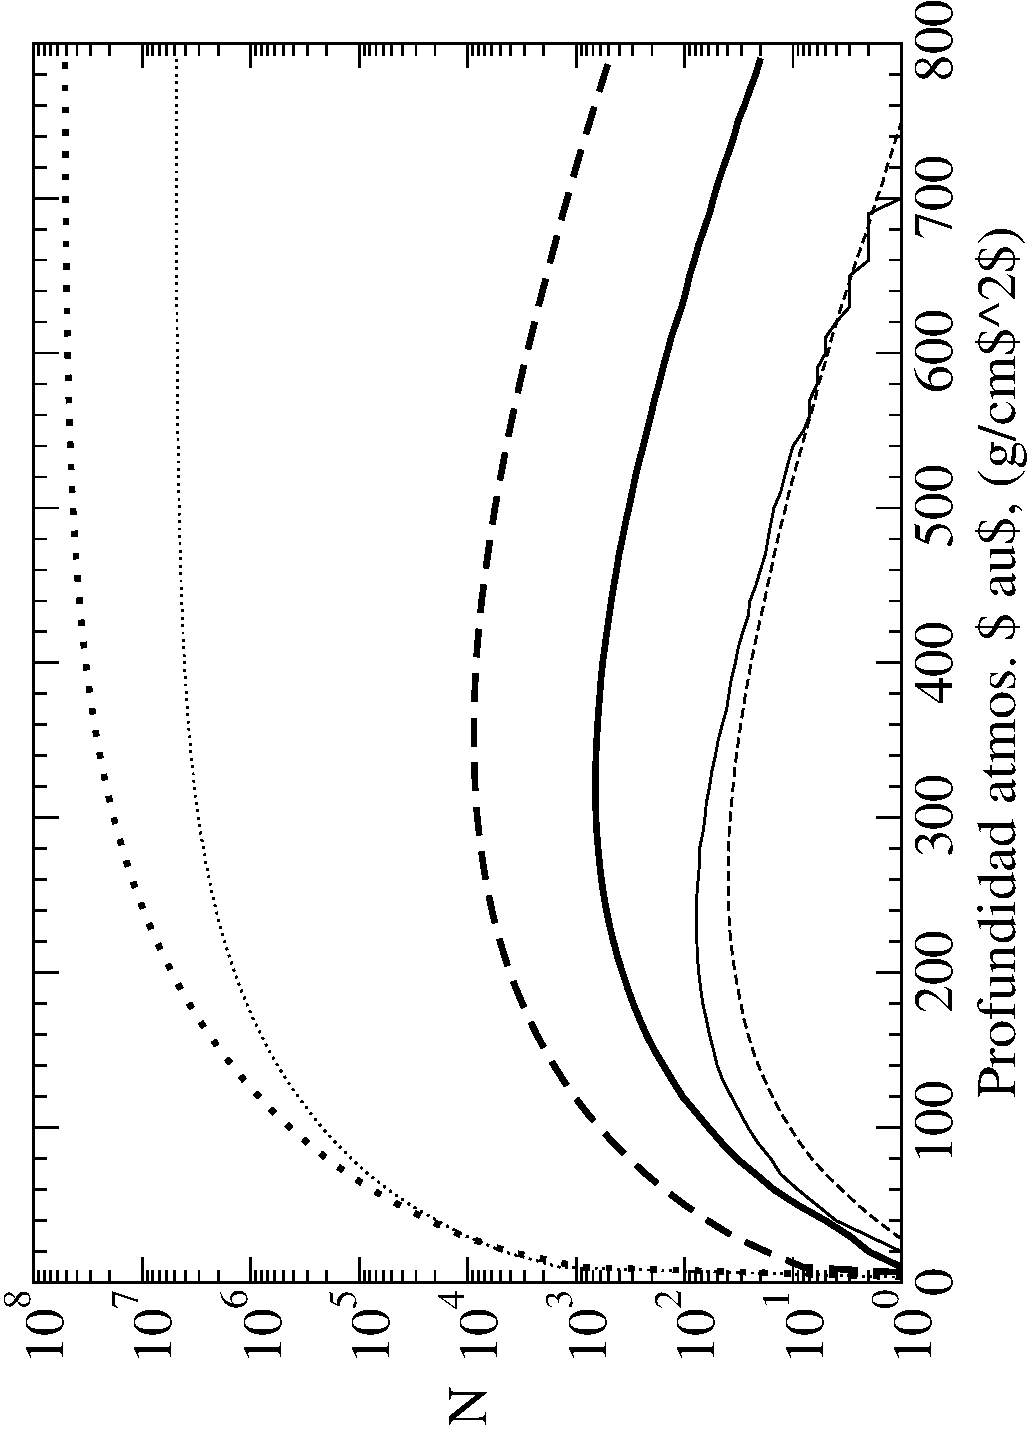
\includegraphics[width=0.35\textwidth,angle=-90,clip]{longdist_100gev-1tev_e}
\hfill
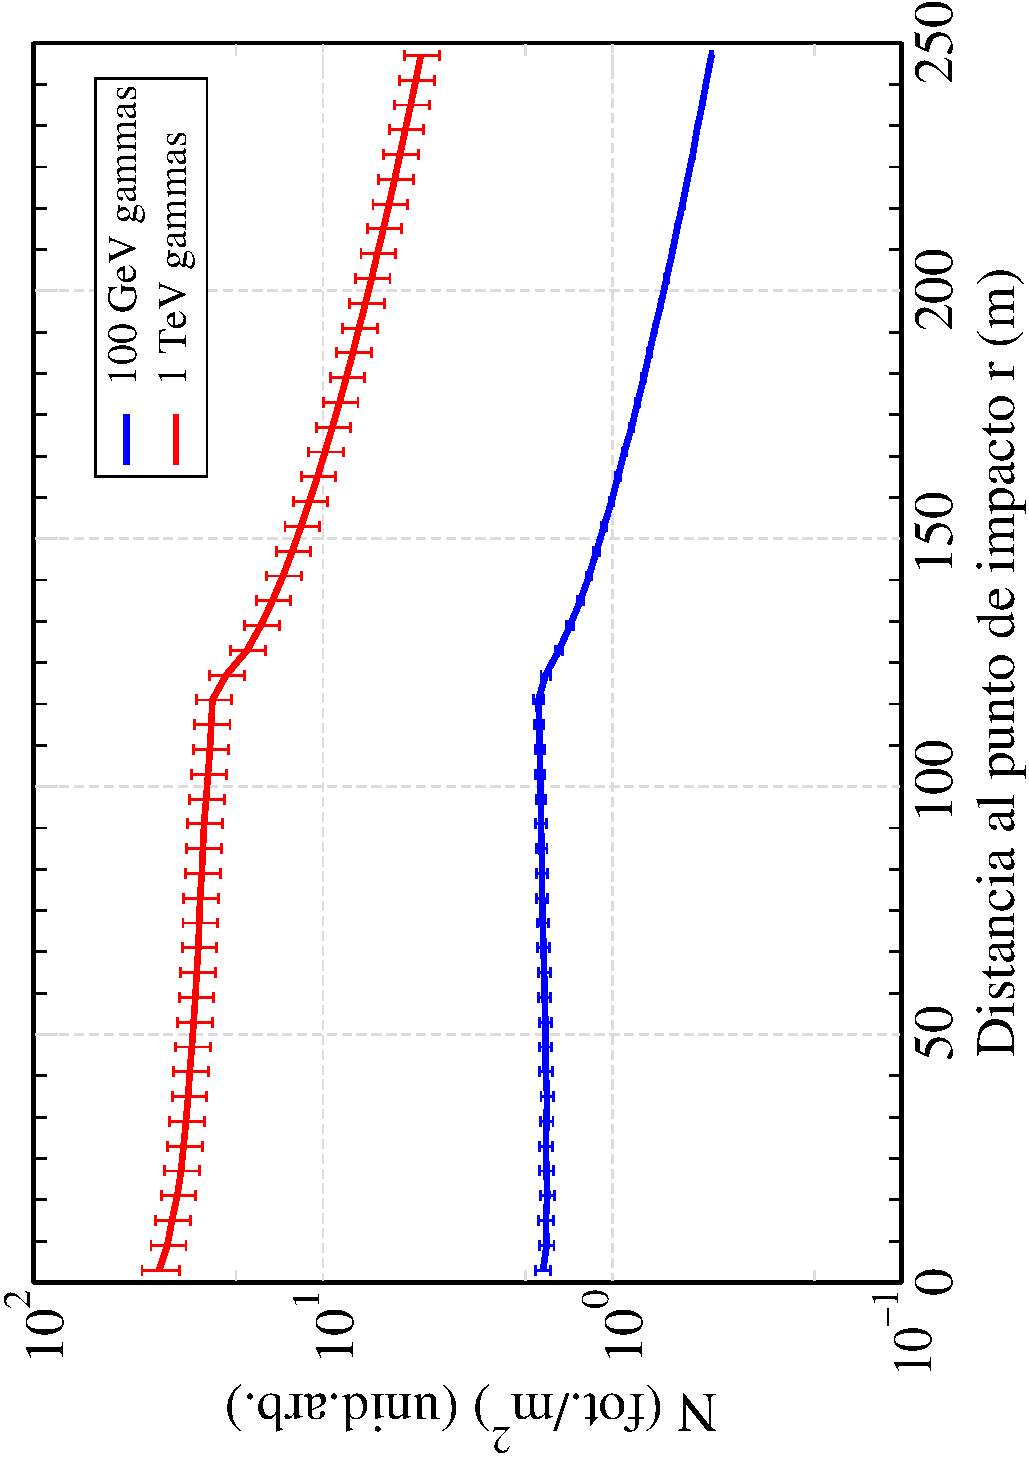
\includegraphics[width=0.35\textwidth,angle=-90,clip]{latdist_100gev-1tev_e}
\fi
\hfill\\
~ \hfill (a) \hfill ~ \hfill (b) \hfill ~\\
\ifenglish
\caption[Example of longitudinal and lateral distributions]%
  {Example of longitudinal and lateral distributions of particles in
  100\u{GeV} and 1\u{TeV} gamma showers}
\else
\caption[Ejemplo de distribuciones longitudinales y laterales]
  {Ejemplo de distribuciones longitudinales y laterales de part'iculas
  en cascadas generadas por rayos gamma de 100\u{GeV} y 1\u{TeV}}
\fi
\label{fig:samplelonglatdist}
\end{figure}
}

%%%%%%%%%%%%%%%%%%%%%%%%%%%%%%%%%%%%%%%%%%%%%%%%%%%%%%%%%%%%
\def\cherenkovfig{
\begin{figure}[tb]
\begin{minipage}{.4\textwidth}%mbox{}
\ifenglish
\center{\includegraphics[width=\textwidth]{cherprincip}}
\caption[Diagram of the Conical \Cherenkov Wavefront]{Diagram of 
  the Conical \Cherenkov Wavefront. The \Cherenkov angle is indicated
  by $\theta_c$} 
\else
\center{\includegraphics[width=\textwidth]{cherprincip_e}}
\caption[Diagrama del frente c'onico de luz \Cherenkov]{Diagrama 
  del frente c'onico de luz \Cherenkov. El 'angulo \Cherenkov viene
  indicado por $\theta_c$} 
\fi
\label{fig:cherenkov1}
\end{minipage}
\hfill
\begin{minipage}{.55\textwidth}%mbox{}
\center{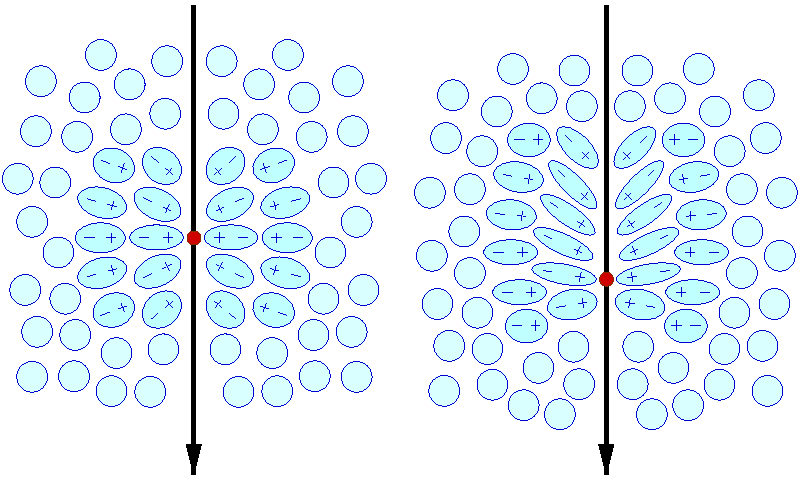
\includegraphics[width=\textwidth]{polariz}\\
~\hfill(a)\hfill~\hfill(b)\hfill~}
\ifenglish
\caption[Schematic view of the polarization process in the atmosphere 
for a relativistic charged particle]{Schematic view of the
  polarization process in the atmosphere when a charged particle is
  moving at high velocity. In (a) the velocity is $\beta\ll 1$, in (b)
  $\beta\simeq 1$} 
\else
\caption[Esquema del proceso de polarizaci'on de las mol'eculas del 
aire al paso de una part'icula cargada relativista]{Esquema del
  proceso de polarizaci'on de las mol'eculas del aire al paso de las
  part'iculas cargadas. En (a) la velocidad es $\beta\ll 1$, en (b)
  $\beta\simeq 1$} 
\fi
\label{fig:polariz}
\end{minipage}
\end{figure}
}

%%%%%%%%%%%%%%%%%%%%%%%%%%%%%%%%%%%%%%%%%%%%%%%%%%%%%%%%%%%%
\def\humpfigsfig{
\begin{figure}[b]
  \centering
  \mbox{}\hfill
  \subfigure[]{%
    \label{fig:humpfocus}\includegraphics[width=.22\textwidth]{humpfocus}}
  \hfill
  \subfigure[]{%
    \label{fig:humpgeom}\includegraphics[width=.35\textwidth]{humpgeom}}
  \hfill\mbox{}
  \ifenglish
  \caption[Focussing \Cherenkov light, and geometrical construction]{(a) 
    Sketch of the focussing of the \Cherenkov light in the atmosphere.
    (b) Geometrical construction used in our \emph{toy-model}.}  \else
  \caption[Efecto de enfoque de la luz \Cherenkov, y construcci'on 
  geom'etrica]{(a) Ilustraci{\'o}n del efecto de enfoque de la luz
    \Cherenkov en la atm'osfera, dando lugar al \emph{hump}. (b)
    Construcci'on geom'etrica usada en nuestros calculos.} \fi
  \label{fig:humpfigs}
\end{figure}
}

%%%%%%%%%%%%%%%%%%%%%%%%%%%%%%%%%%%%%%%%%%%%%%%%%%%%%%%%%%%%
\def\humpldistfig{
\begin{figure}[tb]
  \centering 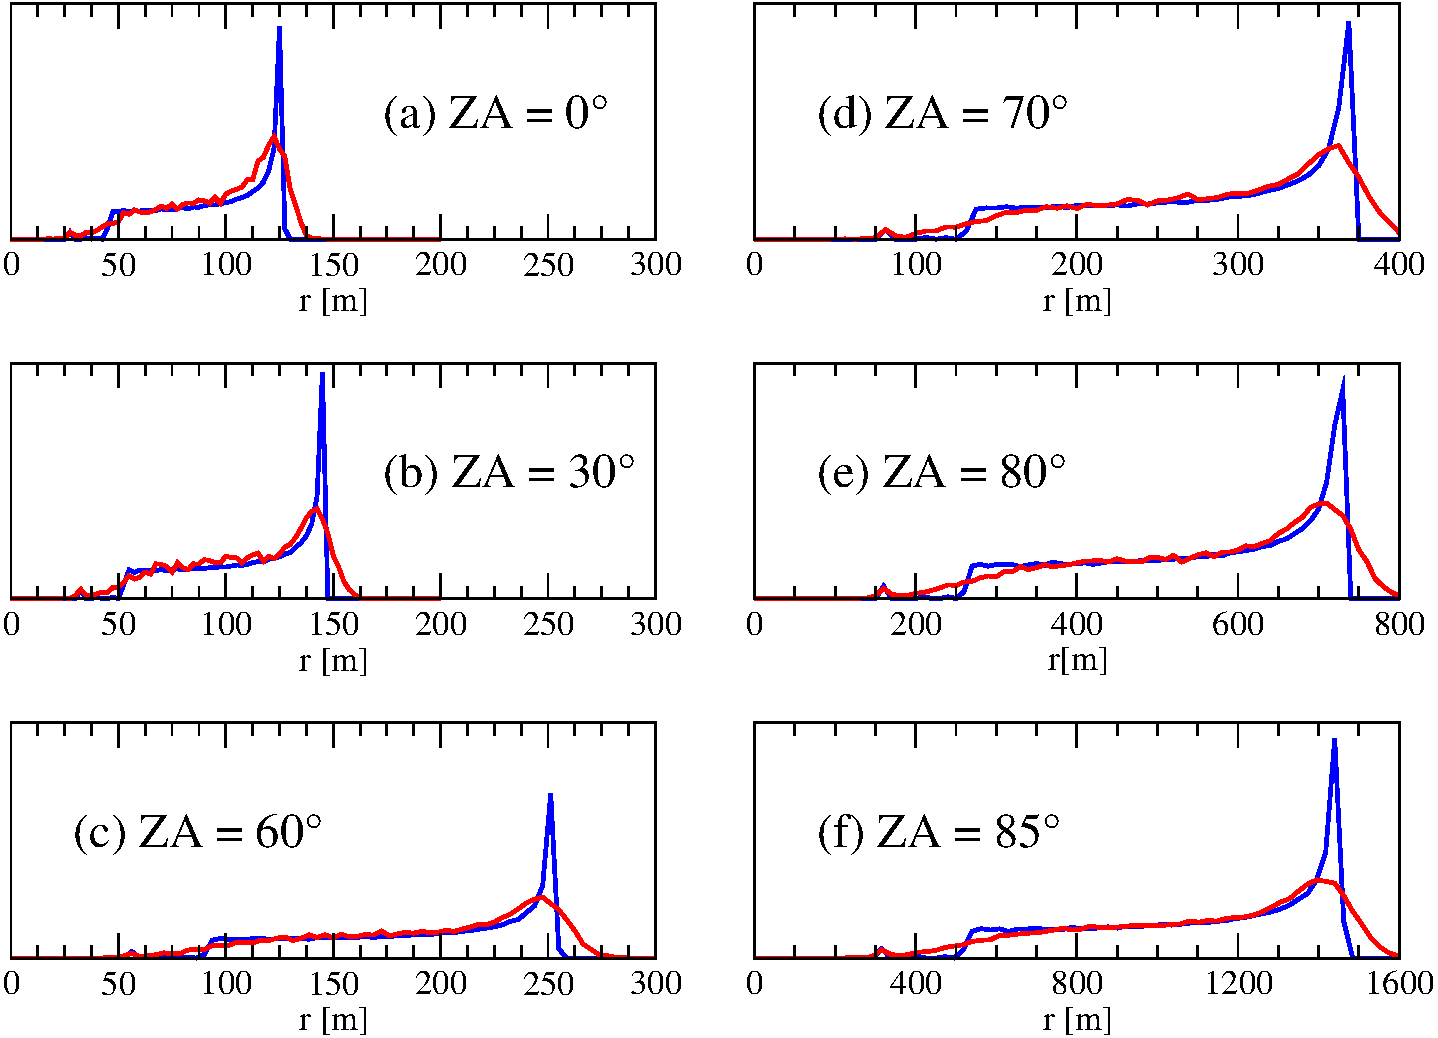
\includegraphics[width=.80\textwidth]{hump_ldist}
  \ifenglish
  \caption[Simple simulation of lateral distributions of \Cherenkov 
  photons]{Histograms of the hits of the \Cherenkov photons in the
    plane perpendicular to the trajectory of the charged particle, for
    different values of the Zenith Angle, in arbitrary units --- in
    blue, without smoothing; in red, with a gaussian smoothing
    function, assuming $\sigma(\theta_{\text{c}}) = 0.05\text{\%}$. Note that in
    the first three histograms, (a)-(c), the scale in the X axis is
    the same, while in the last three, (d)-(f), the scale is
    doubling.} \else
  \caption[Simulaci'on simplista de distribuciones laterales de 
  fotones \Cherenkov]{Histogramas de los puntos de incidencia de
    fotones \Cherenkov en el plano perpendicular a la trayectoria de
    la part'icula cargada inicial, para diversos valores del 'angulo
    cenital, en unidades arbitrarias --- en azul, sin efecto de
    \emph{dispersi'on}; en rojo, con una funci'on de dispersi'on
    gaussiana, tal que $\sigma(\theta_{\text{c}}) = 0.05\text{\%}$.  N'otese que
    en los tres primeros histogramas, (a)-(c), la escala en el eje X
    es identica, mientras que en los tres 'ultimos, (d)-(f), se va
    duplicando al pasar de uno al siguiente.} \fi
  \label{fig:humpldist}
\end{figure}
}

%%%%%%%%%%%%%%%%%%%%%%%%%%%%%%%%%%%%%%%%%%%%%%%%%%%%%%%%%%%%
\def\humpsfig{
\begin{figure}[tb]
  \centering 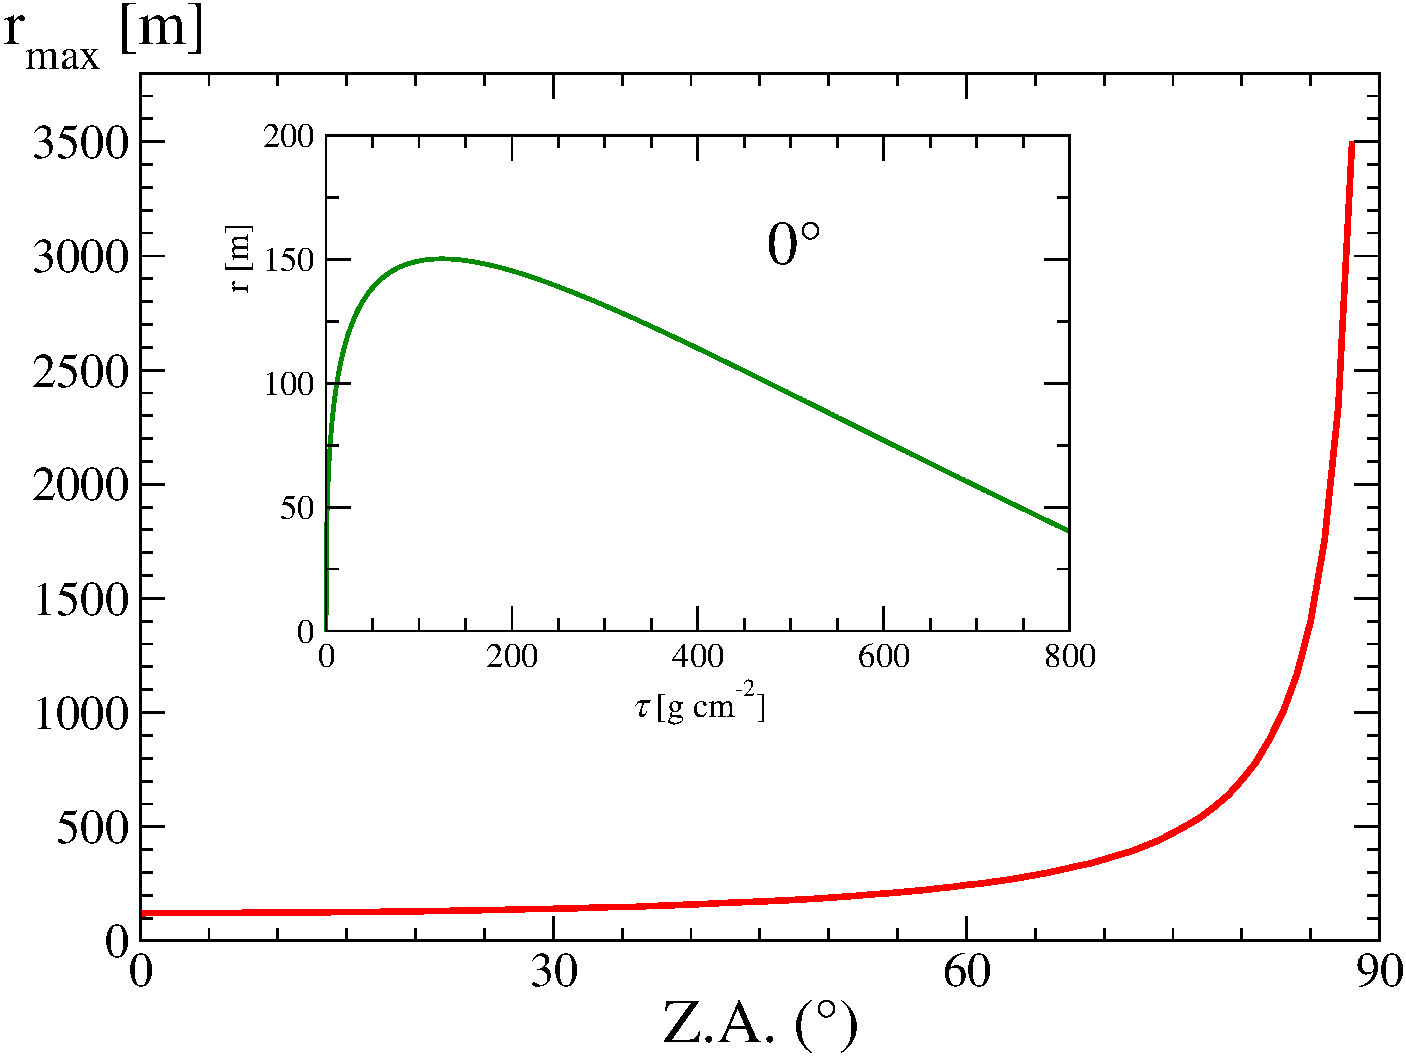
\includegraphics[width=.6\textwidth]{humps}
  \caption{Maxima of the radial distributions of \Cherenkov photons 
    obtained for different initial Zenith Angles. In the embeded
    graph, the theoretical values of the radial distances of the
    emitted \Cherenkov photons are shown as a function of the
    atmospheric thickness $\tau$, for Zenith Angle 0\deg. We can see that
    the theoretical value of the maximum $r$, around $150\u{m}$, is
    very close (and higher) to our calculated value of the position of
    the hump for 0\deg, $r_{\text{max}}\simeq125\u{m}$, as expected.}
  \label{fig:humps}
\end{figure}
}

%%%%%%%%%%%%%%%%%%%%%%%%%%%%%%%%%%%%%%%%%%%%%%%%%%%%%%%%%%%%
%\def\fig{
%}


%%%%%%%%%%%%%%%%%%%%%%%%%%%%%%%%%%%%%%%%%%%%%%%%%%%%%%%%%%%%
%% SIMULATION OF ATMOSPHERIC SHOWERS %%%%%%%%%%%%%%%%%%%%%%%
%%%%%%%%%%%%%%%%%%%%%%%%%%%%%%%%%%%%%%%%%%%%%%%%%%%%%%%%%%%%

%%%%%%%%%%%%%%%%%%%%%%%%%%%%%%%%%%%%%%%%%%%%%%%%%%%%%%%%%%%%
\def\mcsimsample{
\begin{figure}[t]
\centering
\includegraphics[width=0.4\textwidth]{mcsimsample.mps}
\ifenglish
\caption[Schematic flow chart for UNICAS]{Schematic flow chart for a
  version of UNICAS, the core subroutine of one of the first
  simulation programs, developed by J.A. Wrotniak in 1986. This
  routine developed a shower due to the interaction of a single
  nucleon of photon starting at slant height $H_1$, and included
  photoproduction of hadrons. Taken from \cite{Gaisser:book}.}
\else
\caption[Organigrama de la subrutina UNICAS]{Organigrama de la
  subrutina UNICAS, n'ucleo principal de uno de los primeros paquetes
  de simulaci'on de cascadas, desarrollado en 1986 oir J.A. Wrotniak.
  Esta rutina produc'ia cascadas por la interacci'on de un hadr'on o
  fot'on individual, a una altura inclinada $H_1$, e inclu'ia la
  fotoproducci'on de hadrones. Tomado de \cite{Gaisser:book}.}
\fi
\label{fig:MCsimGaisser}
\end{figure}
}

%%%%%%%%%%%%%%%%%%%%%%%%%%%%%%%%%%%%%%%%%%%%%%%%%%%%%%%%%%%%
\def\CORSIKAstructfig{
\begin{figure}[t]
  \begin{center}
    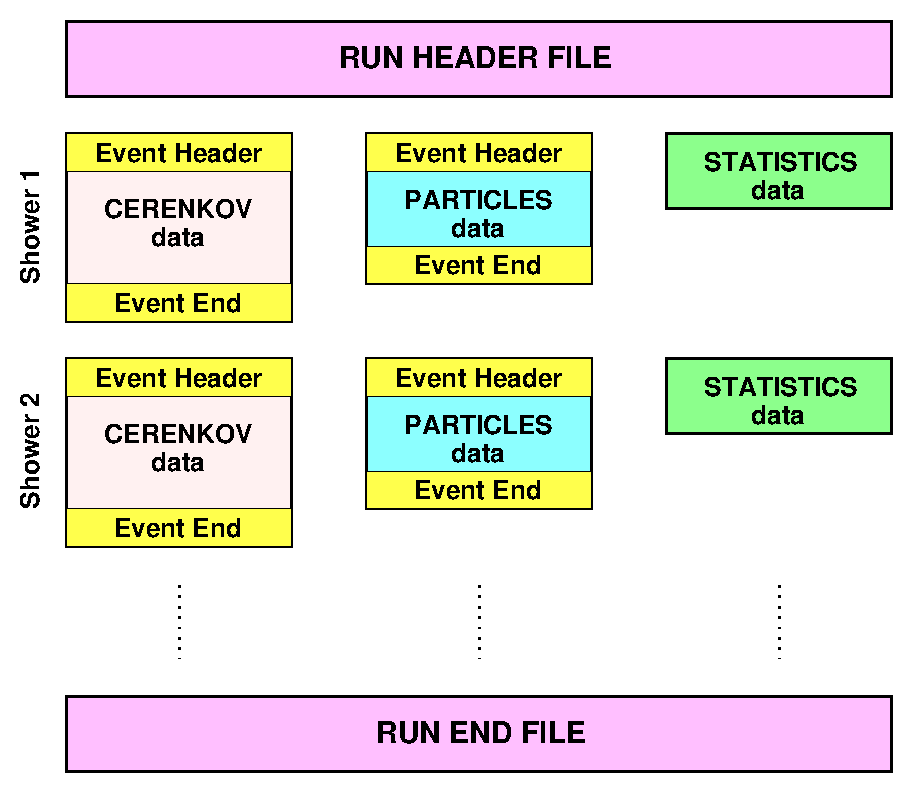
\includegraphics[width=0.5\textwidth]{corsikastruc}
    \caption{Structure of the \CORSIKA output.}
    \label{fig:corsikastruc}
  \end{center}
\end{figure}
}

%%%%%%%%%%%%%%%%%%%%%%%%%%%%%%%%%%%%%%%%%%%%%%%%%%%%%%%%%%%%
\def\CORSIKAinputfig{
\begin{figure}[tb]
\begin{center}
\ttfamily
\scriptsize
\begin{tabular}{lll}
\hline
RUNNR  &1                            & {\rmfamily\itshape number of run} \\
EVTNR  &1                            & {\rmfamily\itshape number of first shower event} \\
NSHOW  &10                           & {\rmfamily\itshape number of showers to generate} \\
PRMPAR &1                            & {\rmfamily\itshape particle type of prim. particle} \\
ESLOPE &0.                           & {\rmfamily\itshape slope of primary energy spectrum} \\
ERANGE &5.E2  5.E2                   & {\rmfamily\itshape energy range of primary particle} \\
THETAP &0.  0.                       & {\rmfamily\itshape range of zenith angle (degree)} \\
PHIP   &0.  0.                       & {\rmfamily\itshape range of azimuth angle (degree)} \\
SEED   &1   0   0                    & {\rmfamily\itshape seed for 1. random number sequence} \\
SEED   &2   0   0                    & {\rmfamily\itshape seed for 2. random number sequence} \\
SEED   &3   0   0                    & {\rmfamily\itshape seed for 3. random number sequence} \\
OBSLEV &2200.E2                      & {\rmfamily\itshape observation level (in cm)} \\
ELMFLG &T   F                        & {\rmfamily\itshape em. interaction flags (NKG,EGS)} \\
RADNKG &200.E2                       & {\rmfamily\itshape outer radius for NKG lat.dens.determ.} \\
ARRANG &0.                           & {\rmfamily\itshape rotation of array to north} \\
FIXHEI &0.  0                        & {\rmfamily\itshape first interaction height \& target} \\
FIXCHI &0.                           & {\rmfamily\itshape starting altitude (g/cm**2)} \\
MAGNET &20.0  42.8                   & {\rmfamily\itshape magnetic field centr. europe} \\
HADFLG &0  0  0  0  0  0             & {\rmfamily\itshape flags for hadr. interaction} \\
GHEISH &T                            & {\rmfamily\itshape use gheisha for low energy hadrons} \\
VENUS  &T                            & {\rmfamily\itshape use venus for high energy hadrons} \\
VENSIG &T                            & {\rmfamily\itshape use VENUS hadronic cross sections} \\
ECUTS  &0.3  0.3  0.020 0.020        & {\rmfamily\itshape energy cuts for particles} \\
MUADDI &T                            & {\rmfamily\itshape additional info for muons} \\
MUMULT &T                            & {\rmfamily\itshape muon multiple scattering angle} \\
LONGI  &T  10.  T                    & {\rmfamily\itshape longit.distr. \& step size \& fit} \\
MAXPRT &10                           & {\rmfamily\itshape max. number of printed events} \\
ECTMAP &1.E4                         & {\rmfamily\itshape cut on gamma factor for printout} \\
STEPFC &10.0                         & {\rmfamily\itshape mult. scattering step length fact.} \\
DEBUG  &F  6  F  1000000             & {\rmfamily\itshape debug flag and log.unit for out} \\
VENDBG &0                            & {\rmfamily\itshape venus debug option} \\
DIRECT &./                           & {\rmfamily\itshape output directory} \\
CWAVLG &290.  600.                   & {\rmfamily\itshape Cherenkov wavelength band} \\
CSCAT  &1  0.  0.                    & {\rmfamily\itshape scatter Cherenkov events} \\
CERSIZ &1.                           & {\rmfamily\itshape bunch size Cherenkov photons} \\
CERFIL &T                            & {\rmfamily\itshape Cherenkov output to extra file} \\
CERTEL &       1                     & {\rmfamily\itshape Number of Cherenkov telescopes (CTs)} \\
       &0. 0. 0. 0. 0. 2000. 1700.   & {\rmfamily\itshape location and size of each CT} \\
EXIT   &                             & {\rmfamily\itshape terminates input} \\
\hline
\end{tabular}
\end{center}
\ifenglish
\caption{Sample \CORSIKA input parameters file}
\else
\caption{Ejemplo de fichero de par'ametros de \CORSIKA}
\fi
\label{fig:corinput}
\end{figure}
}


%%%%%%%%%%%%%%%%%%%%%%%%%%%%%%%%%%%%%%%%%%%%%%%%%%%%%%%%%%%%
%% THE MAGIC TELESCOPE %%%%%%%%%%%%%%%%%%%%%%%%%%%%%%%%%%%%%
%%%%%%%%%%%%%%%%%%%%%%%%%%%%%%%%%%%%%%%%%%%%%%%%%%%%%%%%%%%%

%%%%%%%%%%%%%%%%%%%%%%%%%%%%%%%%%%%%%%%%%%%%%%%%%%%%%%%%%%%%
\def\energygapfig{
\begin{figure}[t]
\centering
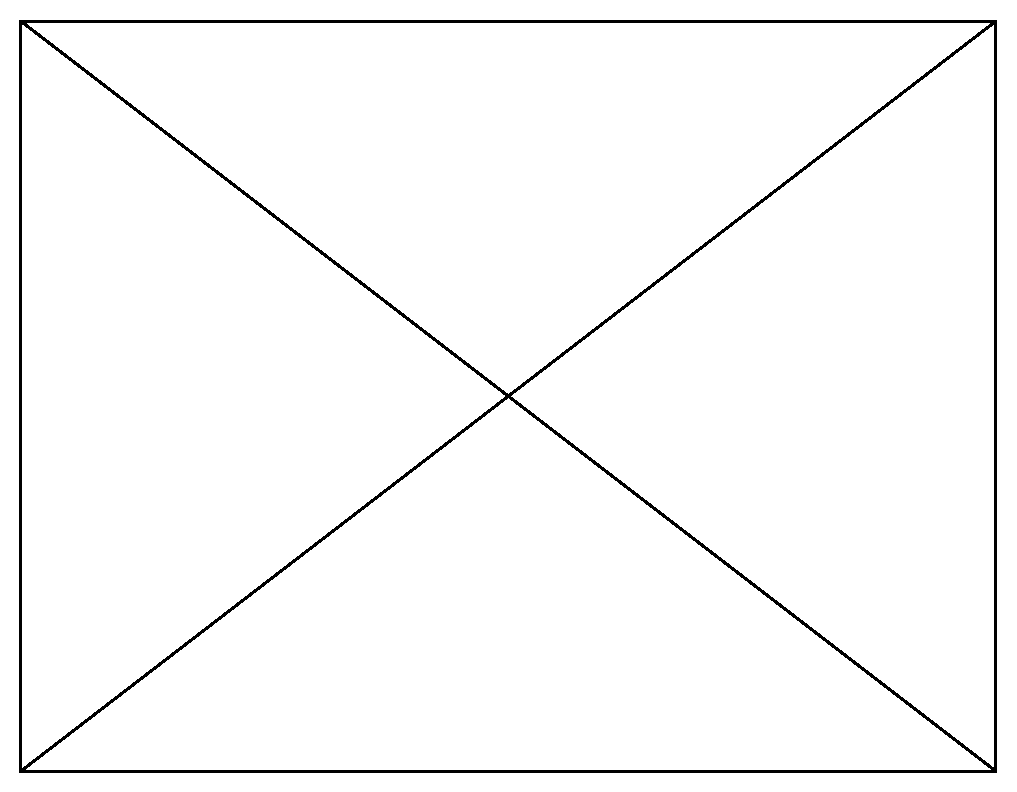
\includegraphics[height=0.4\textwidth,width=0.9\textwidth]{dummy-figure}
\ifenglish
\caption[The covering of the electromagnetic spectrum]{Almost all the
  energies in the electromagnetic spectrum are covered by different
  observation techniques. There is only one energy window still
  unexplored: the range between 10-30 GeV and 100-200 GeV. Covering
  this energy range is the major goal of \MAGIC}
\else
\caption[Cobertura del espectro electromagn'etico]{Casi todos los 
  rangos de energ'ias en el espectro electromagn'etico han sido 
  cubiertos utilizando diferentes t'ecnicas de observaci'on. S'olo 
  existe una ventana energ'etica a'un inexplorada: aquella con 
  energ'ias en el rango 10-30\u{GeV} a 100-200\u{GeV}. El estudio de
  este rango de energ'ias es el principal objetivo de \MAGIC}
\fi
\label{fig:energy_gap}
\end{figure}
}

%%%%%%%%%%%%%%%%%%%%%%%%%%%%%%%%%%%%%%%%%%%%%%%%%%%%%%%%%%%%
\def\CGROenergiesfig{
\begin{figure}[b]
\centering
\ifenglish
\includegraphics[height=0.2\textwidth,width=0.8\textwidth]{CGRO}
\caption{Energy bands covered by the different experiments on board 
  of \I{CGRO}}
\else
\includegraphics[height=0.2\textwidth,width=0.8\textwidth]{CGRO_e}
\caption{Energy bands covered by the different experiments on board 
  of \I{CGRO}}
\fi
\label{fig:CGROenergies}
\end{figure}
}

%%%%%%%%%%%%%%%%%%%%%%%%%%%%%%%%%%%%%%%%%%%%%%%%%%%%%%%%%%%%
\def\MAGICframefig{
\begin{figure}[htb]
\centering
%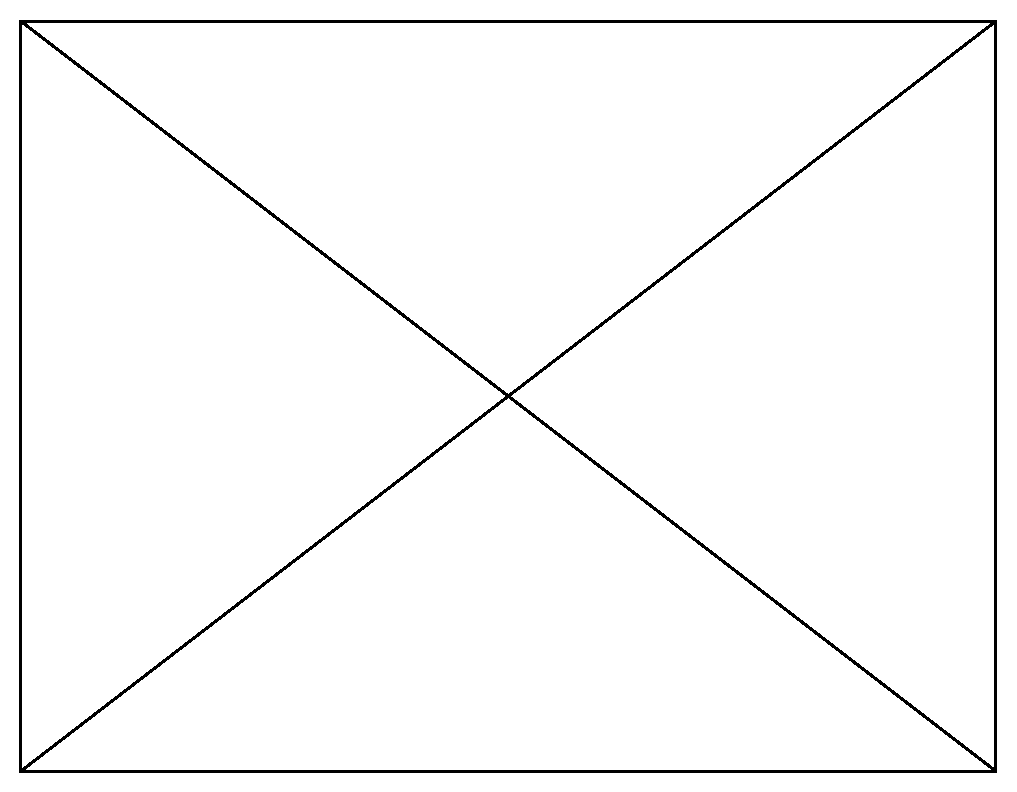
\includegraphics[width=0.495\textwidth]{dummy-figure}\hfill
%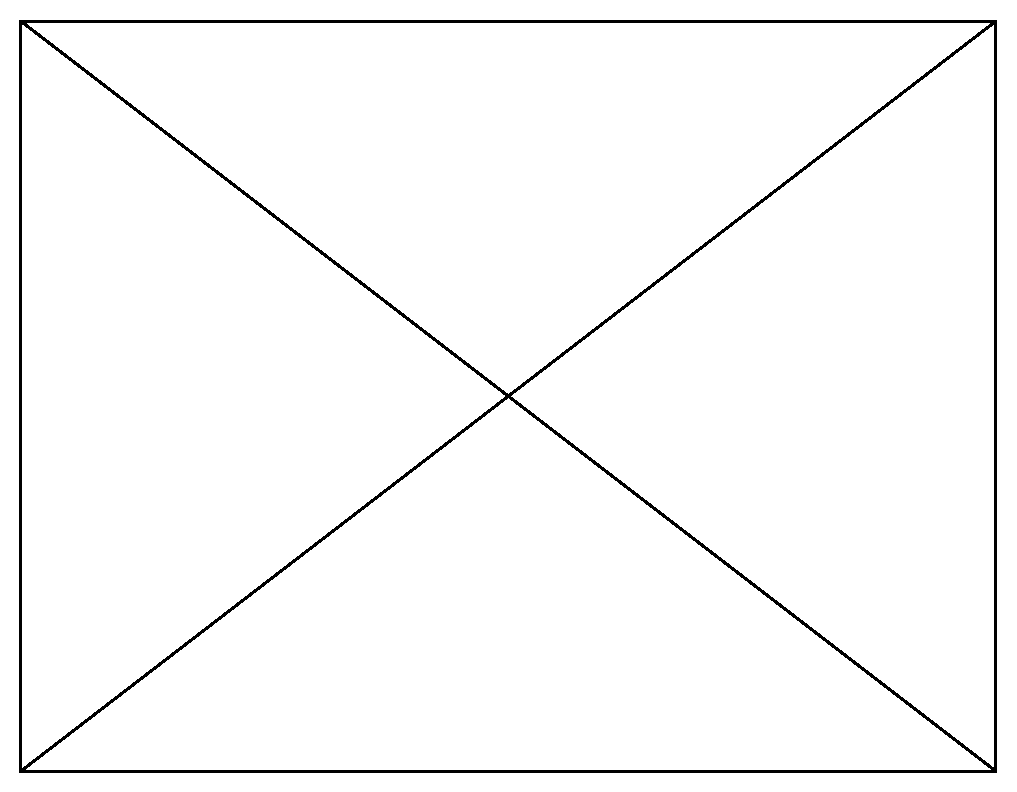
\includegraphics[width=0.495\textwidth]{dummy-figure}\\
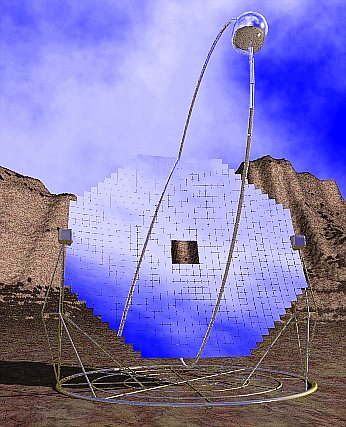
\includegraphics[width=0.48\textwidth]{magiccompview1}\hfill
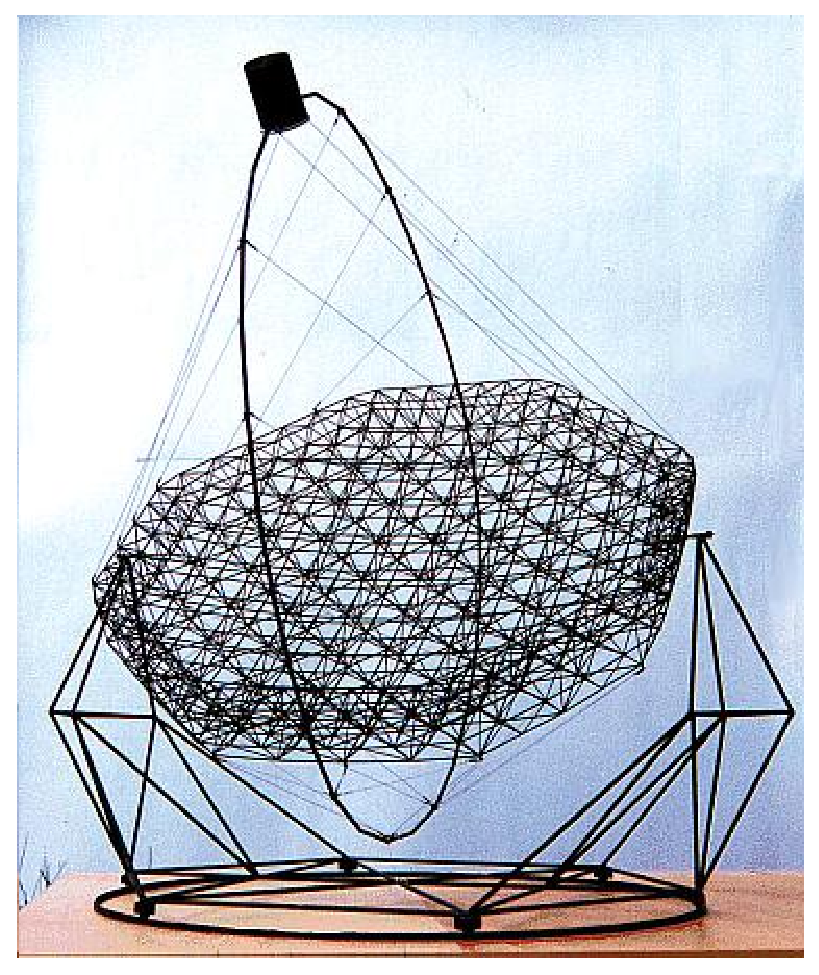
\includegraphics[width=0.48\textwidth]{magic_model}\\
~ \hfill (a) \hfill ~ \hfill (b) \hfill ~\\
\ifenglish
\caption[Computer generated view and photograph of a 1:30 model of 
\MAGIC]{(a) Computer generated view of \MAGIC; (b)
Photograph of a 1:30 model of the \MAGIC telescope; (adapted from
\cite{MAGIC:DR})}
\else
\caption[Imagen generada por ordenador y fotograf'ia de un modelo 
a escala 1:30 de \MAGIC]{(a) Imagen generada por ordenador del disco
  de \MAGIC; (b) Fotograf'ia de un modelo a escala 1:30 del telescopio
  \MAGIC(adaptado de \cite{MAGIC:DR})} \fi
\label{fig:MAGICframe}
\end{figure}
}

%%%%%%%%%%%%%%%%%%%%%%%%%%%%%%%%%%%%%%%%%%%%%%%%%%%%%%%%%%%%
\def\MAGICmirrorcontrol_wfig{
\begin{wrapfigure}[42]{r}{0.50\textwidth}
\centering
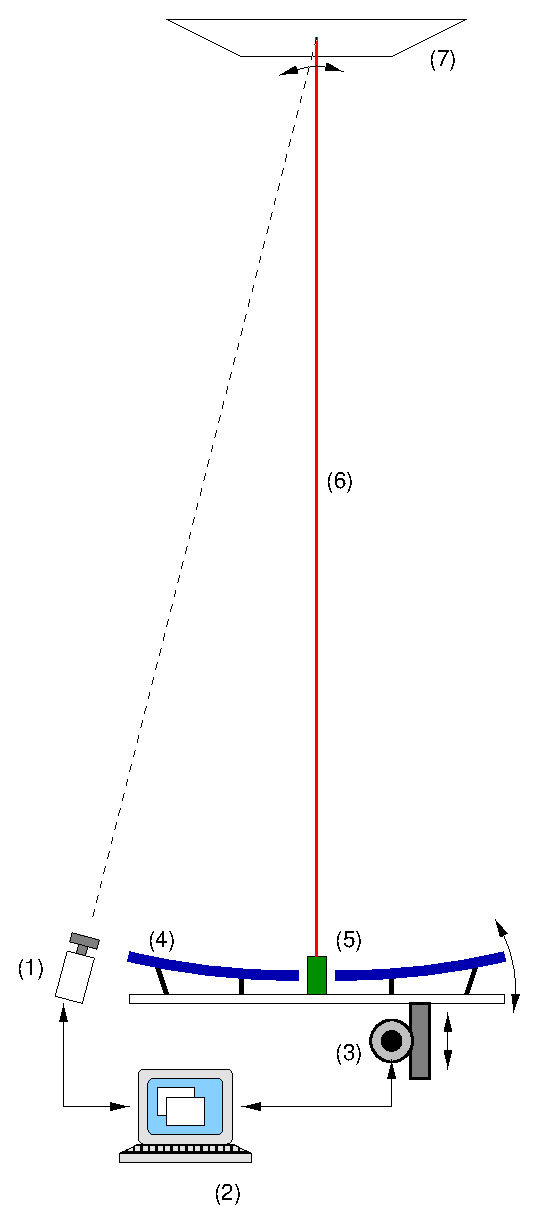
\includegraphics[width=0.45\textwidth]{mirror_control}
\ifenglish
\caption[Schematic view of the active mirror control system of
  \MAGIC]{Schematic view of the active mirror control system of
  \MAGIC: (1) video camera; (2) control computer; (3) stepping motor;
  (4) four-mirror panel; (5) laser pointer; (6) laser beam; and (7)
  focal plane.}
\else
\caption[Visi'on esquem'atica del sistema de control activo de los
  espejos de \MAGIC]{Visi'on esquem'atica del sistema de control
  activo de los espejos de \MAGIC: (1) video c'amara; (2) ordenador de
  control; (3) motor de pasos; (4) soporte para cuatro espejos
  individuales; (5) puntero l'aser; (6) haz l'aser; y (7) plano
  focal.}
\fi
\label{fig:MAGICmirrorcontrol}
\end{wrapfigure}
}

%%%%%%%%%%%%%%%%%%%%%%%%%%%%%%%%%%%%%%%%%%%%%%%%%%%%%%%%%%%%
\def\mirrorsandwichfig{
\begin{figure}[htb]
\centering
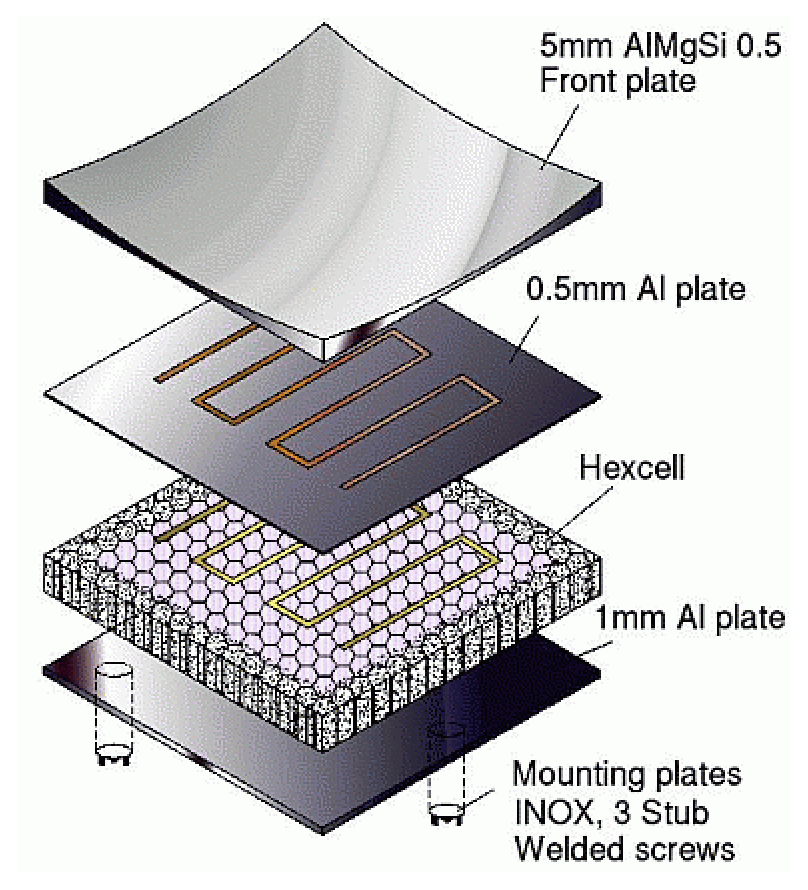
\includegraphics[width=0.6\textwidth]{mirror_element}
\ifenglish
\caption[Exploded view of a mirror element]{Exploded view of a mirror
  element (adapted from \cite{MAGIC:DR})}
\else
\caption[Visi'on detallada de un espejo individual]{Visi'on detallada 
  de un espejo individual (adaptado de \cite{MAGIC:DR})}
\fi
\label{fig:MAGICmirrorsandwich}
\end{figure}
}

%%%%%%%%%%%%%%%%%%%%%%%%%%%%%%%%%%%%%%%%%%%%%%%%%%%%%%%%%%%%
\def\mirrorreflecfig{
\begin{figure}[htb]
\centering
\ifenglish
\includegraphics[width=0.8\textwidth]{mirror_reflec}
\caption[Reflectivity of different mirror surfaces]{Reflectivity 
  of different mirror surfaces (adapted from \cite{MAGIC:DR})} 
\else
\includegraphics[width=0.8\textwidth]{mirror_reflec_e}
\caption[Reflectividades de diferentes superficies de 
  espejos]{Reflectividades de diferentes superficies de espejos
  (adaptado de \cite{MAGIC:DR})} 
\fi
\label{fig:mirrorreflec}
\end{figure}
}

%%%%%%%%%%%%%%%%%%%%%%%%%%%%%%%%%%%%%%%%%%%%%%%%%%%%%%%%%%%%
\def\MAGICcamerafig{
\begin{figure}[htb]
\centering
\includegraphics[width=0.7\textwidth]{magic-camera_4ring}
\ifenglish
\caption[Geometrical pixel pattern of the camera of
\MAGIC]{Geometrical pixel pattern
  of the \MAGIC Telescope's camera, as used in this work}
\else
\caption[Dise~no de pixelizaci'on de la c'amara de 
\MAGIC]{Dise~no de pixelizaci'on de la c'amara de \MAGIC, tal y como
  se ha usado en este trabajo} 
\fi
\label{fig:MAGICcamera}
\end{figure}
}

%%%%%%%%%%%%%%%%%%%%%%%%%%%%%%%%%%%%%%%%%%%%%%%%%%%%%%%%%%%%
\def\QuantumEfffig{
\begin{figure}[hbt]
\centering
\includegraphics[width=0.8\textwidth]{QEs}
\ifenglish
\caption[Spectral Quantum Efficiency for different detection
devices]{Spectral Quantum Efficiency for different detection devices.
  The lines are spline approximations (adapted from \cite{MAGIC:DR})}
\else
\caption[Eficiencia Cu'antica espectral para diferentes dispositivos]
{Eficiencia Cu'antica espectral para diferentes dispositivos de
  detecci'on. Las l'ineas dibujadas son aproximaciones por splines
  (adaptado de \cite{MAGIC:DR})} 
\fi
\label{fig:QE}
\end{figure}
}

%%%%%%%%%%%%%%%%%%%%%%%%%%%%%%%%%%%%%%%%%%%%%%%%%%%%%%%%%%%%
\def\pixelreadoutfig{
\begin{figure}[hbt]
\centering
\ifenglish
\includegraphics[width=0.9\textwidth]{pixel_readout}
\caption[Basic block diagram of a single camera pixel readout
  chain]{Basic block diagram of a single camera pixel readout chain
  (taken from \cite{MAGIC:DR})}
\else
\includegraphics[width=0.9\textwidth]{pixel_readout_e}
\caption[Diagr'ama b'asico de bloques de la secuencia de lectura de un
  pixel individual]{Diagr'ama b'asico de bloques de la secuencia de
  lectura de un pixel individual (tomado de \cite{MAGIC:DR})}
\fi
\label{fig:pixelreadout}
\end{figure}
}

%%%%%%%%%%%%%%%%%%%%%%%%%%%%%%%%%%%%%%%%%%%%%%%%%%%%%%%%%%%%
%% SIMULATION OF THE MAGIC TELESCOPE %%%%%%%%%%%%%%%%%%%%%%%
%%%%%%%%%%%%%%%%%%%%%%%%%%%%%%%%%%%%%%%%%%%%%%%%%%%%%%%%%%%%

%%%%%%%%%%%%%%%%%%%%%%%%%%%%%%%%%%%%%%%%%%%%%%%%%%%%%%%%%%%%
\def\simprocessfig{
\begin{wrapfigure}[20]{r}{0.55\textwidth}
%\begin{figure}[t]
\centering
\ifenglish
\includegraphics[height=0.58\textwidth]{simprocess}
\caption[Scheme of the simulation process]{Scheme of the global steps
  taken in the simulation process}
\else
\includegraphics[height=0.58\textwidth]{simprocess_e}
\caption[Esquema del proceso de simulci'on]{Visi'on esquem'atica de los
  pasos contemplados en el proceso de simulaci'on}
\fi
\label{fig:simprocess}
%\end{figure}
\end{wrapfigure}
}

%%%%%%%%%%%%%%%%%%%%%%%%%%%%%%%%%%%%%%%%%%%%%%%%%%%%%%%%%%%%
\def\coordsysfig{
\begin{figure}[t]
\centering
\ifenglish
\includegraphics[width=0.6\textwidth]{coord}
\caption[Coordinate systems and angles in the simulation]{Coordinate systems
  and angles used in the simulation programs. There are three main
  coordinate systems, $S \equiv OXYZ$, $S' \equiv OX'Y'Z'$ and
  $S"\equiv O"X"Y"Z"$ (see text). For the systems $S'$ and $S"$ the
  axes $Y'$ and $Y"$ have been omitted for clarity} 
\else
\includegraphics[width=0.6\textwidth]{coord_e}
\caption['Angulos y systemas de coordenadas de la simulaci'on]{'Angulos
  y systemas de coordenadas usados en los progamas de simulaci'on.
  Existen tres sistemas principales, $S \equiv OXYZ$, $S' \equiv
  OX'Y'Z'$ y $S"\equiv O"X"Y"Z"$ (ver texto). Para los systemas $S'$ y
  $S"$, los ejes $Y'$ y $Y"$ se han omitido en la figura para mayor
  claridad.}  
\fi
\label{fig:coordsys}
\end{figure}
}

%%%%%%%%%%%%%%%%%%%%%%%%%%%%%%%%%%%%%%%%%%%%%%%%%%%%%%%%%%%%
\def\geomviewfig{
\begin{wrapfigure}[22]{r}{0.45\textwidth}
%\begin{figure}[b!]
\centering
\includegraphics[width=0.55\linewidth]{geomview}
\ifenglish
\caption[Geometrical construction for an observer looking at a source
under a Zenith Angle $\theta$]{This geometrical construction
  illustrates the situation for an observer located at A, looking at a
  source under a Zenith Angle $\theta$}
\else
\caption[Escenario para un observador apuntando a una fuente bajo un 
'angulo cenital $\theta$]{Esta construcci'on geom'etrica ilustra el
  escenario en el que un observador situado en A apunta su telescopio
  hacia la una fuente que se encuentra a un 'angulo cenital $\theta$}
\fi
\label{fig:geomview}
%\end{figure}
\end{wrapfigure}
}

%%%%%%%%%%%%%%%%%%%%%%%%%%%%%%%%%%%%%%%%%%%%%%%%%%%%%%%%%%%%
%\def\Systemsfig{ %% this is done in landscape, so we use \textheight
%\begin{landscape}
%\begin{figure}[t]
%\begin{minipage}[b]{14cm}%mbox{}
%\centering
%\ifenglish
%\includegraphics[width=0.7\linewidth]{coord}
%\caption[Coordinate systems and angles in the simulation]{Coordinate systems
%  and angles used in the simulation programs. There are three main
%  coordinate systems, $S \equiv OXYZ$, $S' \equiv OX'Y'Z'$ and
%  $S"\equiv O"X"Y"Z"$ (see text). For the systems $S'$ and $S"$ the
%  axes $Y'$ and $Y"$ have been omitted for clarity} 
%\else
%\includegraphics[width=0.7\linewidth]{coord_e}
%\caption['Angulos y systemas de coordenadas de la simulaci'on]{'Angulos
%  y systemas de coordenadas usados en los progamas de simulaci'on.
%  Existen tres sistemas principales, $S \equiv OXYZ$, $S' \equiv
%  OX'Y'Z'$ y $S"\equiv O"X"Y"Z"$ (ver texto). Para los systemas $S'$ y
%  $S"$, los ejes $Y'$ y $Y"$ se han omitido en la figura para mayor
%  claridad.}  
%\fi
%\label{fig:coordsys}
%\end{minipage}
%\begin{minipage}[b]{8cm}%mbox{}
%\centering
%\includegraphics[width=0.9\linewidth]{geomview}
%\ifenglish
%\caption[Geometrical construction for an observer looking at a source
%under a Zenith Angle $\theta$]{This geometrical construction
%  illustrates the situation for an observer located at A, looking at a
%  source under a Zenith Angle $\theta$}
%\else
%\caption[Escenario para un observador apuntando a una fuente bajo un 
%'angulo cenital $\theta$]{Esta construcci'on geom'etrica ilustra el
%  escenario en el que un observador situado en A apunta su telescopio
%  hacia la una fuente que se encuentra a un 'angulo cenital $\theta$}
%\fi
%\label{fig:geomview}
%\end{minipage}
%\end{figure}
%\end{landscape}
%}

%%%%%%%%%%%%%%%%%%%%%%%%%%%%%%%%%%%%%%%%%%%%%%%%%%%%%%%%%%%%
\def\Systemsfig{ %% this is done in landscape, so we use \textheight
%\begin{landscape}
\begin{figure}[p]
\begin{narrow}{-1.5cm}{-1cm}
\setlength{\narrowlength}{\linewidth}
\begin{sideways}
\parbox[b]{13.5cm}{
\centering
\ifenglish
%\includegraphics[width=0.95\linewidth]{coord}
\includegraphics[height=.87\narrowlength]{coord}
\caption[Coordinate systems and angles in the simulation]{Coordinate systems
  and angles used in the simulation programs. There are three main
  coordinate systems, $S \equiv OXYZ$, $S' \equiv OX'Y'Z'$ and
  $S"\equiv O"X"Y"Z"$ (see text). For the systems $S'$ and $S"$ the
  axes $Y'$ and $Y"$ have been omitted for clarity} 
\else
\includegraphics[width=0.95\linewidth]{coord_e}
\caption['Angulos y systemas de coordenadas de la simulaci'on]{'Angulos
  y systemas de coordenadas usados en los progamas de simulaci'on.
  Existen tres sistemas principales, $S \equiv OXYZ$, $S' \equiv
  OX'Y'Z'$ y $S"\equiv O"X"Y"Z"$ (ver texto). Para los systemas $S'$ y
  $S"$, los ejes $Y'$ y $Y"$ se han omitido en la figura para mayor
  claridad.}  
\fi
\label{fig:coordsys}}
\hfill
\parbox[b]{8cm}{
\centering
%\includegraphics[width=0.95\linewidth]{geomviewmp}
\includegraphics[height=.87\narrowlength]{geomviewmp}
\ifenglish
\caption[Geometrical construction for an observer looking at a source
under a Zenith Angle $\theta$]{This geometrical construction
  illustrates the situation for an observer located at A, looking at a
  source under a Zenith Angle $\theta$} \else
\caption[Escenario para un observador apuntando a una fuente bajo un 
'angulo cenital $\theta$]{Esta construcci'on geom'etrica ilustra el
  escenario en el que un observador situado en A apunta su telescopio
  hacia la una fuente que se encuentra a un 'angulo cenital $\theta$} \fi
\label{fig:geomview}}
\end{sideways}
\end{narrow}
\end{figure}
%\end{landscape}
}

%%%%%%%%%%%%%%%%%%%%%%%%%%%%%%%%%%%%%%%%%%%%%%%%%%%%%%%%%%%%%
%\def\hvdiffsfig{
%\begin{figure}[htbp]
%\includegraphics[width=0.49\linewidth]{deg-difference}
%\hfill
%\includegraphics[width=0.49\linewidth]{differences}\\
%\mbox{}\hfill(a)\hfill\mbox{}\hfill(b)\hfill\mbox{} 
%\ifenglish
%\caption[Difference of vertical heights \hv and $h_{\mathrm{v,approx}}$]%
%{Difference of vertical heights \hv and $h_{\mathrm{v,approx}}$ for
%  $\ho=0\u{km}$ and $\ho=2.2\u{km}$: (a) as a function of the Zenith
%  Angle, for different values of \hc; and (b) as a function of \hc,
%  for different Zenith Angles.}  
%\else
%\caption[Diferencia entre alturas verticales \hv y $h_{\mathrm{v,approx}}$]%
%{Diferencia entre alturas verticales \hv y $h_{\mathrm{v,approx}}$,
%  para $\ho=0\u{km}$ y $\ho=2.2\u{km}$: (a) en funci'on del 'angulo
%  cenital, para diferentes valores de \hc; y (b) en funci'on de \hc,
%  para varios 'angulos cenitales} 
%\fi
%\label{fig:hvdiffs}
%\end{figure}
%}

%%%%%%%%%%%%%%%%%%%%%%%%%%%%%%%%%%%%%%%%%%%%%%%%%%%%%%%%%%%%
\def\hvdiffsfig{
\begin{wrapfigure}[16]{r}{0.55\textwidth}
\includegraphics[width=0.55\textwidth]{hvdif}
\ifenglish
\caption[Difference of vertical heights \hv and $h_{\mathrm{v,approx}}$]%
{Difference of vertical heights \hv and $h_{\mathrm{v,approx}}$, when
  $\ho=2.2\u{km}$. The figure shows the value of $\Delta\hv$ (see
  text), as a function of the height \hc and the Zenith Angle. Below
  85\deg the difference is well below the 5\%.}  \else
\caption[Diferencia entre alturas verticales \hv y $h_{\mathrm{v,approx}}$]%
{Diferencia entre alturas verticales \hv y $h_{\mathrm{v,approx}}$,
  cuando $\ho=2.2\u{km}$. La figura muestra el valor de $\Delta\hv$
  (ver texto), en funci'on de la altura \hc y el 'angulo cenital. Por
  debajo de 85\deg la diferencia se encuentra siempre por debajo del
  5\%} 
\fi
\label{fig:hvdiffs}
\end{wrapfigure}
}

%%%%%%%%%%%%%%%%%%%%%%%%%%%%%%%%%%%%%%%%%%%%%%%%%%%%%%%%%%%%
\def\AMcompfig{
\begin{figure}[p]
\includegraphics[width=0.49\linewidth]{am0}
\hfill
\includegraphics[width=0.49\linewidth]{am4}\\
\mbox{}\hfill(a)\hfill\mbox{}\hfill(b)\hfill\mbox{} \\
\mbox{}\hfill
\includegraphics[width=0.49\linewidth]{am22}
\hfill\mbox{}\\
\mbox{}\hfill(c)\hfill\mbox{} 
\ifenglish
\caption[Comparison of $m$, $m_{\mathrm{simple}}$ and
$\mathcal{AM}_{\mathrm{refraction}}$]{Comparison of $m$,
  $m_{\mathrm{simple}}$ and $\mathcal{AM}_{\mathrm{refraction}}$,
  using two values for the vertical height ($\hv=5\u{km}$ and
  $\hv=100\u{km}$), as a function of the Zenith Angle (only values
  above 70\deg are shown), for three observation levels: (a)
  $\ho=0\u{km}$, (b) $\ho=4\u{km}$, and (c) $\ho=2.2\u{km}$.}  
\else
\caption[Comparaci'on de los valores de $m$, $m_{\mathrm{simple}}$ y
$\mathcal{AM}_{\mathrm{refraction}}$]{Comparaci'on de los valores de
  $m$, $m_{\mathrm{simple}}$ y $\mathcal{AM}_{\mathrm{refraction}}$,
  tal y como han sido calculados en el texto, usando dos valores de la
  altura en la vertical ($\hv=5\u{km}$ y $\hv=100\u{km}$), en funci'on
  del 'angulo cenital (s'olo se muestran los valores por encima de
  70\deg), y para tres niveles de observaci'on: (a) $\ho=0\u{km}$, (b)
  $\ho=4\u{km}$, y (c) $\ho=2.2\u{km}$.}  
\fi
\label{fig:AMcomp}
\end{figure}
}

%%%%%%%%%%%%%%%%%%%%%%%%%%%%%%%%%%%%%%%%%%%%%%%%%%%%%%%%%%%%%
%\def\collimationfigs{
%\begin{figure}[t]
%\begin{minipage}[c]{0.5\textwidth}%mbox{}
%\centering
%\includegraphics[width=\textwidth]{collimation}
%\ifenglish
%\caption{Illustration of the \emph{collimation} effect in \MAGIC.}
%\else 
%\caption{Ilustraci'on del efecto \emph{colimaci'on} in \MAGIC.}
%\fi
%\label{fig:collimation}
%\end{minipage}
%\begin{minipage}[c]{0.48\textwidth}%mbox{}
%\centering
%\includegraphics[width=\linewidth]{colldelta}
%\ifenglish
%\caption[Displacement of the camera position as a function of the
%distance of the mirror to the optical axis of \MAGIC]{Value of the
%  displacement of the camera position, $\delta$, in order to get an
%  optimal focussing, as a function of the distance of the mirror to
%  the optical axis of \MAGIC, $r$.} 
%\else
%\caption[Desplazamiento de la c'amara en funci'on de la 
%distancia del espejo al eje 'optico de \MAGIC]{Valor del
%  desplazamiento de la posici'on de la c'amara, $\delta$, para obtener
%  un enfoque 'optimo, en funci'on de la distancia del espejo al eje
%  'optico de \MAGIC, $r$.}  
%\fi
%\end{minipage}
%\end{figure}
%}

%%%%%%%%%%%%%%%%%%%%%%%%%%%%%%%%%%%%%%%%%%%%%%%%%%%%%%%%%%%%
\def\collimationfig{
\begin{wrapfigure}[39]{r}{0.45\textwidth}
%\begin{floatingfigure}{0.45\textwidth}
%\begin{figure}[p]
\centering
\vskip -20pt
\includegraphics[width=0.43\textwidth]{collimation}
%\includegraphics[height=0.8\textheight]{collimation}
\ifenglish
\caption{Illustration of the \emph{collimation} effect in \MAGIC.}
\else 
\caption{Ilustraci'on del efecto \emph{colimaci'on} in \MAGIC.}
\fi
\label{fig:collimation}
%\end{figure}
%\end{floatingfigure}
\end{wrapfigure}
}

%%%%%%%%%%%%%%%%%%%%%%%%%%%%%%%%%%%%%%%%%%%%%%%%%%%%%%%%%%%%
\def\colldeltafig{
\begin{figure}[b]
\centering
\includegraphics[width=0.55\textwidth]{colldelta}
\ifenglish
\caption[Displacement of the camera position as a function of the
distance of the mirror to the optical axis of \MAGIC]{Value of the
  displacement of the camera position, $\delta$, in order to get an
  optimal focussing, as a function of the distance of the mirror to
  the optical axis of \MAGIC, $r$.} 
\else
\caption[Desplazamiento de la c'amara en funci'on de la 
distancia del espejo al eje 'optico de \MAGIC]{Valor del
  desplazamiento de la posici'on de la c'amara, $\delta$, para obtener
  un enfoque 'optimo, en funci'on de la distancia del espejo al eje
  'optico de \MAGIC, $r$.}  
\fi
\label{fig:colldelta}
\end{figure}
}

%%%%%%%%%%%%%%%%%%%%%%%%%%%%%%%%%%%%%%%%%%%%%%%%%%%%%%%%%%%%%
%\def\hfinfhlfivekmfig{
%\begin{figure}[p]
%  \centering
%  \includegraphics[width=0.6\textwidth]{hfinf-hl5km}
%  \caption{Image of a point-like source of light at 5\u{km}, when the 
%    telescope is focussed at infinity}
%  \label{fig:hfinfhlfivekm}
%\end{figure}}

%%%%%%%%%%%%%%%%%%%%%%%%%%%%%%%%%%%%%%%%%%%%%%%%%%%%%%%%%%%%%
%\def\hfinfhltenkmfig{
%\begin{figure}[p]
%  \centering
%  \includegraphics[width=0.6\textwidth]{hfinf-hl10km}
%  \caption{Image of a point-like source of light at 10\u{km}, when the 
%    telescope is focussed at infinity}
%  \label{fig:hfinfhltenkm}
%\end{figure}}

%%%%%%%%%%%%%%%%%%%%%%%%%%%%%%%%%%%%%%%%%%%%%%%%%%%%%%%%%%%%%
%\def\hfinfhltwelvekmfig{
%\begin{figure}[p]
%  \centering
%  \includegraphics[width=0.6\textwidth]{hfinf-hl12km}
%  \caption{Image of a point-like source of light at 12\u{km}, when the 
%    telescope is focussed at infinity}
%  \label{fig:hfinfhltwelvekm}
%\end{figure}}

%%%%%%%%%%%%%%%%%%%%%%%%%%%%%%%%%%%%%%%%%%%%%%%%%%%%%%%%%%%%%
%\def\hfinfhlhundredkmfig{
%\begin{figure}[p]
%  \centering
%  \includegraphics[width=0.6\textwidth]{hfinf-hl100km}
%  \caption{Image of a point-like source of light at 100\u{km}, when the 
%    telescope is focussed at infinity}
%  \label{fig:hfinfhlhundredkm}
%\end{figure}}

%%%%%%%%%%%%%%%%%%%%%%%%%%%%%%%%%%%%%%%%%%%%%%%%%%%%%%%%%%%%%
%\def\hfinfhlinffig{
%\begin{figure}[p]
%  \centering
%  \includegraphics[width=0.6\textwidth]{hfinf-hlinf}
%  \caption{Image of a point-like source of light at infinity, when the 
%    telescope is focussed at infinity}
%  \label{fig:hfinfhlinf}
%\end{figure}}

%%%%%%%%%%%%%%%%%%%%%%%%%%%%%%%%%%%%%%%%%%%%%%%%%%%%%%%%%%%%%
%\def\hftenkmhlfivekmfig{
%\begin{figure}[p]
%  \centering
%  \includegraphics[width=0.6\textwidth]{hf10km-hl5km}
%  \caption{Image of a point-like source of light at 5\u{km}, when the 
%    telescope is focussed at 10\u{km}}
%  \label{fig:hftenmkhlfivekm}
%\end{figure}}

%%%%%%%%%%%%%%%%%%%%%%%%%%%%%%%%%%%%%%%%%%%%%%%%%%%%%%%%%%%%%
%\def\hftenkmhltenkmfig{
%\begin{figure}[p]
%  \centering
%  \includegraphics[width=0.6\textwidth]{hf10km-hl10km}
%  \caption{Image of a point-like source of light at 10\u{km}, when the 
%    telescope is focussed at 10\u{km}}
%  \label{fig:hftenmkhltenkm}
%\end{figure}}

%%%%%%%%%%%%%%%%%%%%%%%%%%%%%%%%%%%%%%%%%%%%%%%%%%%%%%%%%%%%%
%\def\hftenkmhltwelvekmfig{
%\begin{figure}[p]
%  \centering
%  \includegraphics[width=0.6\textwidth]{hf10km-hl12km}
%  \caption{Image of a point-like source of light at 12\u{km}, when the 
%    telescope is focussed at 10\u{km}}
%  \label{fig:hftenmkhltwelvekm}
%\end{figure}}

%%%%%%%%%%%%%%%%%%%%%%%%%%%%%%%%%%%%%%%%%%%%%%%%%%%%%%%%%%%%%
%\def\hftenkmhlhundredkmfig{
%\begin{figure}[p]
%  \centering
%  \includegraphics[width=0.6\textwidth]{hf10km-hl100km}
%  \caption{Image of a point-like source of light at 100\u{km}, when the 
%    telescope is focussed at 10\u{km}}
%  \label{fig:hftenmkhlhundredkm}
%\end{figure}}

%%%%%%%%%%%%%%%%%%%%%%%%%%%%%%%%%%%%%%%%%%%%%%%%%%%%%%%%%%%%%
%\def\hftenkmhlinffig{
%\begin{figure}[p]
%  \centering
%  \includegraphics[width=0.6\textwidth]{hf10km-hlinf}
%  \caption{Image of a point-like source of light at infinity, when the 
%    telescope is focussed at 10\u{km}}
%  \label{fig:hftenmkhlinf}
%\end{figure}}

%%%%%%%%%%%%%%%%%%%%%%%%%%%%%%%%%%%%%%%%%%%%%%%%%%%%%%%%%%%%
\def\hlfivekmfig{
\begin{figure}[p]
  \centering
  \ifCOLORversion
    \includegraphics[width=0.49\linewidth]{hfinf-hl5km}\hfill
    \includegraphics[width=0.49\linewidth]{hf10km-hl5km}\\
  \else
    \includegraphics[width=0.49\linewidth]{hfinf-hl5km-bw}\hfill
    \includegraphics[width=0.49\linewidth]{hf10km-hl5km-bw}\\
  \fi
  \mbox{}\hfill(a)\hfill\mbox{}\hfill(b)\hfill\mbox{} \\
  \ifenglish
  \caption[Image of a point-like source of light located at 
  5\u{km}]{Image of a point-like source of light located at 5\u{km} on
    the axis of the telescope, in different image planes, at both
    sides of the focal plane of the reflector: (a) when the telescope
    is focussed at infinity; and (b) when the telescope is focussed at
    10\u{km}} \else
  \caption[Imagen de una fuente puntual situada a 5\u{km}]{Imagen 
    de una fuente puntual situada a 5\u{km} en el eje del telescopio,
    vista en diferentes planos de proyecci'on a ambos lados del plano
    focal del reflector: (a) cuando el telescopio est{\'a} enfocado al
    infinito; y (b) cuando est{\'a} enfocado a 10\u{km}} \fi
  \label{fig:hlfivekm}
\end{figure}}

%%%%%%%%%%%%%%%%%%%%%%%%%%%%%%%%%%%%%%%%%%%%%%%%%%%%%%%%%%%%
\def\hltenkmfig{
\begin{figure}[p]
  \centering
  \ifCOLORversion
    \includegraphics[width=0.49\linewidth]{hfinf-hl10km}\hfill
    \includegraphics[width=0.49\linewidth]{hf10km-hl10km}\\
  \else
    \includegraphics[width=0.49\linewidth]{hfinf-hl10km-bw}\hfill
    \includegraphics[width=0.49\linewidth]{hf10km-hl10km-bw}\\
  \fi
  \mbox{}\hfill(a)\hfill\mbox{}\hfill(b)\hfill\mbox{} \\
  \ifenglish
  \caption[Image of a point-like source of light located at 
  10\u{km}]{Image of a point-like source of light located at 10\u{km}
    on the axis of the telescope, in different image planes, at both
    sides of the focal plane of the reflector: (a) when the telescope
    is focussed at infinity; and (b) when the telescope is focussed at
    10\u{km}} \else
  \caption[Imagen de una fuente puntual situada a 10\u{km}]{Imagen 
    de una fuente puntual situada a 10\u{km} en el eje del telescopio,
    vista en diferentes planos de proyecci'on a ambos lados del plano
    focal del reflector: (a) cuando el telescopio est{\'a} enfocado al
    infinito; y (b) cuando est{\'a} enfocado a 10\u{km}} \fi
  \label{fig:hltenkm}
\end{figure}}

%%%%%%%%%%%%%%%%%%%%%%%%%%%%%%%%%%%%%%%%%%%%%%%%%%%%%%%%%%%%
\def\hltwelvekmfig{
\begin{figure}[p]
  \centering
  \ifCOLORversion
    \includegraphics[width=0.49\linewidth]{hfinf-hl12km}\hfill
    \includegraphics[width=0.49\linewidth]{hf10km-hl12km}\\
  \else
    \includegraphics[width=0.49\linewidth]{hfinf-hl12km-bw}\hfill
    \includegraphics[width=0.49\linewidth]{hf10km-hl12km-bw}\\
  \fi
  \mbox{}\hfill(a)\hfill\mbox{}\hfill(b)\hfill\mbox{} \\
  \ifenglish
  \caption[Image of a point-like source of light located at 
  12\u{km}]{Image of a point-like source of light located at 12\u{km}
    on the axis of the telescope, in different image planes, at both
    sides of the focal plane of the reflector: (a) when the telescope
    is focussed at infinity; and (b) when the telescope is focussed at
    10\u{km}} \else
  \caption[Imagen de una fuente puntual situada a 12\u{km}]{Imagen 
    de una fuente puntual situada a 12\u{km} en el eje del telescopio,
    vista en diferentes planos de proyecci'on a ambos lados del plano
    focal del reflector: (a) cuando el telescopio est{\'a} enfocado al
    infinito; y (b) cuando est{\'a} enfocado a 10\u{km}} \fi
  \label{fig:hltwelvekm}
\end{figure}}

%%%%%%%%%%%%%%%%%%%%%%%%%%%%%%%%%%%%%%%%%%%%%%%%%%%%%%%%%%%%
\def\hlhundredkmfig{
\begin{figure}[p]
  \centering
  \ifCOLORversion
    \includegraphics[width=0.49\linewidth]{hfinf-hl100km}\hfill
    \includegraphics[width=0.49\linewidth]{hf10km-hl100km}\\
  \else
    \includegraphics[width=0.49\linewidth]{hfinf-hl100km-bw}\hfill
    \includegraphics[width=0.49\linewidth]{hf10km-hl100km-bw}\\
  \fi
  \mbox{}\hfill(a)\hfill\mbox{}\hfill(b)\hfill\mbox{} \\
  \ifenglish
  \caption[Image of a point-like source of light located at 
  100\u{km}]{Image of a point-like source of light located at
    100\u{km} on the axis of the telescope, in different image planes,
    at both sides of the focal plane of the reflector: (a) when the
    telescope is focussed at infinity; and (b) when the telescope is
    focussed at 10\u{km}} \else
  \caption[Imagen de una fuente puntual situada a 100\u{km}]{Imagen 
    de una fuente puntual situada a 100\u{km} en el eje del
    telescopio, vista en diferentes planos de proyecci'on a ambos
    lados del plano focal del reflector: (a) cuando el telescopio est{\'a}
    enfocado al infinito; y (b) cuando est{\'a} enfocado a 10\u{km}} \fi
  \label{fig:hlhundredkm}
\end{figure}}

%%%%%%%%%%%%%%%%%%%%%%%%%%%%%%%%%%%%%%%%%%%%%%%%%%%%%%%%%%%%
\def\hlinffig{
\begin{figure}[p]
  \centering
  \ifCOLORversion
    \includegraphics[width=0.49\linewidth]{hfinf-hlinf}\hfill
    \includegraphics[width=0.49\linewidth]{hf10km-hlinf}\\
  \else
    \includegraphics[width=0.49\linewidth]{hfinf-hlinf-bw}\hfill
    \includegraphics[width=0.49\linewidth]{hf10km-hlinf-bw}\\
  \fi
  \mbox{}\hfill(a)\hfill\mbox{}\hfill(b)\hfill\mbox{} \\
  \ifenglish
  \caption[Image of a point-like source of light located at 
  infinity]{Image of a point-like source of light located at infinity
    on the axis of the telescope, in different image planes, at both
    sides of the focal plane of the reflector: (a) when the telescope
    is focussed at infinity; and (b) when the telescope is focussed at
    10\u{km}} \else
  \caption[Imagen de una fuente puntual en el infinito]{Imagen 
    de una fuente puntual en el infinito, en el eje del telescopio,
    vista en diferentes planos de proyecci'on a ambos lados del plano
    focal del reflector: (a) cuando el telescopio est{\'a} enfocado al
    infinito; y (b) cuando est{\'a} enfocado a 10\u{km}} \fi
  \label{fig:hlinf}
\end{figure}}

%%%%%%%%%%%%%%%%%%%%%%%%%%%%%%%%%%%%%%%%%%%%%%%%%%%%%%%%%%%%
\def\Mspotsfig{
\begin{figure}[p]
  \centering
  {\mbox{}\hspace{10cm}\includegraphics[width=2cm]{testbmp}}\\[-25pt]
  \ifCOLORversion
  \includegraphics[width=\textwidth]{Mspots}
  \else
  \includegraphics[width=\textwidth]{Mspots-bw}
  \fi
  \ifenglish
  \caption[Image of a letter \texttt{M} enclosed in a square, in the camera 
  plane]{Image of a letter \texttt{M} enclosed in a square, in the
    camera plane (see above, the light comes from the white areas).
    The image is projected from a lamp located at height above the
    observation level of 10\u{km}, with the telescope pointing to the
    Zenith. The area on the ground covered by the image is just
    slightly larger that the dish of \MAGIC. The different images
    correspond to different distances of the projection plane to the
    dish, from 1692\u{cm} to 1707\u{cm} (see text). Note that the
    scale is normalized to the maximum concentration of light (for
    1700\u{cm})} \else
  \caption[Imagen de la letra \texttt{M} rodeada por un cuadrado]{Imagen 
    de la letra \texttt{M} rodeada por un cuadrado, en el plano focal
    (v'ease encima la imagen original; la luz proviene de las 'aeras
    en blanco).  The image se envia desde un proyector situado a
    10\u{km} por encima del nivel de observaci'on, en la vertical del
    telescopio, con 'este apuntando al cenit. El 'area cubierta en el
    suelo es ligeramente mayor que el tama~no del espejo de \MAGIC.
    Las diferentes im'agenes corresponden a distintas distancias entre
    el centro del espejo y el plano de la imagen, desde 1692\u{cm} a
    1707\u{cm} (ver texto).  N'otese que la escala se ha normalizado a
    la m'axima concentraci'on de luz (obtenida para 1700\u{cm})} \fi
  \label{fig:Mspots}
\end{figure}
}

%%%%%%%%%%%%%%%%%%%%%%%%%%%%%%%%%%%%%%%%%%%%%%%%%%%%%%%%%%%%
\def\thetaspotsfig{
\begin{figure}[p]
  \centering
  \ifCOLORversion
    \includegraphics[width=0.8\textwidth]{theta-spots}
  \else
    \includegraphics[width=0.8\textwidth]{theta-spots-bw}
  \fi
  \ifenglish
  \caption[Image of a point-like light source for different 
  angles]{Image of a point-like light source located at 10\u{km} above
    the observation level, in the axis of \MAGIC, with the telescope
    pointing to the Zenith. Different \emph{off-axis} angles have
    simulated used, from 0\deg to 2.5\deg. The different rows of
    images correspond to: (a) perfect system, reflectivity 100\%; (b)
    to (f) realistic system, reflectivity 90\%, scatter in the
    orientation of individual mirrors from 0\u{mm} to 5\u{mm} in the
    camera plane (see text). Note that we have used a logarithmic
    scale (normalized to the case of the maximum concentration of
    light --- obtained for the first spot, 0\deg, in (a)).}  
\else
  \caption[Imagen de una fuente puntual de luz a 10\u{km}]{Imagen de una
    fuente puntual de luz a 10\u{km} situada a 10\u{km} por encima del
    nivel de observaci'on, en el eje del telescopio, con 'este
    apuntando al cenit. Se han usado varios 'angulos \emph{off-axis}
    de incidencia de la luz, desde 0\deg hasta 2.5\deg. Las diferentes
    filas de im'agenes corresponden a: (a) sistema perfecto,
    reflectividad 100\%; (b) a (f) sistema realista, reflectividad
    90\%, desviaciones aleatorias del apuntado de los ejes de los
    espejos de 0\u{mm} a 5\u{mm}, en el plano de la c'amara (ver
    texto). N'otese que en esta figura se ha utilizado una escala de
    intensidades de luz logar'itmica, normalizada al caso de m'axima
    concentraci'on de luz --- obtenida para la primera imagen, 0\deg,
    del caso (a).}  \fi
  \label{fig:thetaspots}
\end{figure}
}

%%%%%%%%%%%%%%%%%%%%%%%%%%%%%%%%%%%%%%%%%%%%%%%%%%%%%%%%%%%%
\def\zonesfig{
\begin{figure}[p]
\centering 
\ifenglish
\includegraphics[width=0.8\textwidth]{magic_focalsview}
\caption[Division of the mirrors of \MAGIC in different zones]{The 
  whole set of mirrors in \MAGIC is divided in eight different zones,
  having all the mirrors in a given zone a common focal length. This
  focal length increases with the radius of the zone (see Table
  \ref{tbl:zonefocals}).}  \else
\includegraphics[width=0.8\textwidth]{magic_focalsview_e}
\caption[Agrupamiento de los espejos de \MAGIC en diferentes 
zonas]{Los espejos de \MAGIC han sido agrupados en ocho zonas. Cada
  una de las zonas viene caracterizada por una distancia focal com'un
  para todos sus espejos. Esta distancia focal aumenta con el radio de
  la zona (v'ease tabla \ref{tbl:zonefocals}).}  \fi
\label{fig:zones}
\end{figure}
}

%%%%%%%%%%%%%%%%%%%%%%%%%%%%%%%%%%%%%%%%%%%%%%%%%%%%%%%%%%%%
\def\zonesfocalsfig{
\begin{figure}[p]
\centering
\ifenglish
\includegraphics[width=0.8\textwidth]{nfocals}
\caption{Histogram of focal lengths in different zones}
\else 
\includegraphics[width=0.8\textwidth]{nfocals_e}
\caption{Histograma de las longitudes focales de las diferentes 
  zonas}
\fi
\label{fig:zonesfocals}
\end{figure}
}

%%%%%%%%%%%%%%%%%%%%%%%%%%%%%%%%%%%%%%%%%%%%%%%%%%%%%%%%%%%%
\def\axesfigs{
\begin{figure}[t]
\begin{minipage}[b]{0.48\textwidth}%mbox{}
\centering
\includegraphics[width=0.95\textwidth]{pixels}
\ifenglish
\caption{Tri-axis hexagonal coordinate system 
   used in the pixel characterization}
\else
\caption{Systema de coordenadas tri-axial usado en la 
  identificaci'on de los p'ixeles}
\fi
\label{fig:triaxis}
\end{minipage}
\hfill
\begin{minipage}[b]{0.48\textwidth}%mbox{}
\centering
\includegraphics[width=0.95\textwidth]{pixelspre}
\ifenglish
\caption{Bi-axis coordinate system 
  used in the pixel numbering, and in the calculation of the
  coordinates of the centers of the pixels} 
\else
\caption{Systema de coordenadas bi-axial usado en la 
  numeraci'on de los p'ixeles, y en el c{\'a}lculo de las posiciones de
  los centros} 
\fi
\label{fig:biaxis}
\end{minipage}
\end{figure}
}

%%%%%%%%%%%%%%%%%%%%%%%%%%%%%%%%%%%%%%%%%%%%%%%%%%%%%%%%%%%%%
%\def\triaxisfig{
%\begin{figure}[htb]
%\centering
%\includegraphics[width=0.8\textwidth]{pixels}
%\ifenglish
%\caption{Tri-axis hexagonal coordinate system 
%   used in the pixel characterization}
%\else
%\caption{Systema de coordenadas tri-axial usado en la 
%  identificaci'on de los p'ixeles}
%\fi
%\label{fig:triaxis}
%\end{figure}
%}

%%%%%%%%%%%%%%%%%%%%%%%%%%%%%%%%%%%%%%%%%%%%%%%%%%%%%%%%%%%%%
%\def\biaxisfig{
%\begin{figure}[htb]
%\centering
%\includegraphics[width=0.8\textwidth]{pixelspre}
%\ifenglish
%\caption{Bi-axis coordinate system 
%  used in the pixel numbering, and in the calculation of the
%  coordinates of the centers of the pixels} 
%\else
%\caption{Systema de coordenadas bi-axial usado en la 
%  numeraci'on de los p'ixeles, y en el c{\'a}lculo de las posiciones de
%  los centros} 
%\fi
%\label{fig:biaxis}
%\end{figure}
%}

%%%%%%%%%%%%%%%%%%%%%%%%%%%%%%%%%%%%%%%%%%%%%%%%%%%%%%%%%%%%
%\def\qealgorfig{
%\begin{figure*}[tb]
%  \begin{center}
%    \includegraphics[width=0.25\textwidth]{qefig1bis}
%    \caption{Simple algorithm to simulate the conversion of incoming
%      photons into photoelectrons in a photocathode with a given Quantum
%      Efficiency \QE.}
%    \label{fig:algorithm1}
%  \end{center}
%\end{figure*}
%}

%%%%%%%%%%%%%%%%%%%%%%%%%%%%%%%%%%%%%%%%%%%%%%%%%%%%%%%%%%%%
\def\noutphotfig{
\begin{figure}[p]
  \begin{center}
    \includegraphics[width=0.7\textwidth]{qehistqe}
    \ifenglish
    \caption[Distributions of number of photoelectrons for several 
    \QE]{Distributions of the number of outcoming photoelectrons
      (\Ntrial, solid line; \Nrand, dashed line) for different values
      of \QE. In this case, $\Nphot=1000$.}  
    \else
    \caption[Distribuciones de fotoelectrones para diferentes 
    \QE]{Distributiones del n'umero de fotoelectrones resultantes
      (\Ntrial, l'inea continua; \Nrand, l'inea discontinua) para
      varios valoers de \QE. En este caso se ha fijado $\Nphot=1000$.}
    \fi
    \label{fig:distrib1}
  \end{center}
\end{figure}
}

%%%%%%%%%%%%%%%%%%%%%%%%%%%%%%%%%%%%%%%%%%%%%%%%%%%%%%%%%%%%
\def\noutqesmallfig{
\begin{figure}[p]
  \begin{center}
    \includegraphics[width=0.6\textwidth]{varwithp}
    \ifenglish
    \caption[Distributions of \Ntrial for  $\QEo=0.2$]{Distributions 
      of the number of outcoming photoelectrons (\Ntrial) for
      different values of \Nphot (in these cases
      $\log_{10}\Nphot=0.5,1.0,1.5\text{ and }3.0$), using a
      $\QEo=0.2$.}  
    \else
    \caption[Distribuciones resultantes de \Ntrial para 
    $\QEo=0.2$]{Distribuciones del n'umero de fotoelectrones
      resultantes (\Ntrial) para varios valores de \Nphot (en la
      figura se han usado los valores
      $\log_{10}\Nphot=0.5,1.0,1.5\text{ y }3.0$), con una
      $\QEo=0.2$.}  
    \fi
    \label{fig:varwithp}
  \end{center}
\end{figure}
}

%%%%%%%%%%%%%%%%%%%%%%%%%%%%%%%%%%%%%%%%%%%%%%%%%%%%%%%%%%%%
\def\varquotfig{
\begin{figure}[p]
  \begin{center}
    \includegraphics[width=0.4\textwidth,angle=-90,clip=]{varwithqe}
    \ifenglish
    \caption[Variation of $z$ with \QEo]{Variation of the quotient 
      $z=\sigma(\Nrand)/\sigma(\Ntrial)$ with different values of
      \QEo, also in the case of $\Nphot=1000$. The curve is very
      similar for other values of \Nphot .}  \else
    \caption[Variaci'on de $z$ con \Qeo]{Variaci'on del cociente 
      $z=\sigma(\Nrand)/\sigma(\Ntrial)$ con el valor de \QEo, en el
      caso $\Nphot=1000$. Para otros valores de \Nphot la curva es muy
      similar.}  
    \fi
    \label{fig:varwithqe}
  \end{center}
\end{figure}
}

%%%%%%%%%%%%%%%%%%%%%%%%%%%%%%%%%%%%%%%%%%%%%%%%%%%%%%%%%%%%
\def\vonneumannfig{
\begin{figure}[p]
  \begin{center}
    \includegraphics[width=0.5\textwidth,clip=]{qefig2}
    \ifenglish
    \caption[Ilustration of the \emph{Acceptance-Rejection Method} (Von
    Neumann)]{Ilustration of the \emph{Acceptance-Rejection Method}
      (Von Neumann), for an arbitrary probability density function.
      The pairs of random numbers $(x,y)$ will cover the area below
      the line $y=C/(b-a)$. Only those below the curve $S(x)$ will be
      accepted.}  \else
    \caption[Ilustraci'on del \emph{M'etodo Aceptaci'on-Rechazo} 
    (o de Von Neumann)]{Ilustraci'on del \emph{M'etodo
        Aceptaci'on-Rechazo} (o de Von Neumann), para una funci'on
      densidad de probabilidad arbitraria. Los pares de n'umeros
      aleatorios $(x,y)$ cubren el area por debajo de la l'inea
      $y=C/(b-a)$. S'olo aquellos pares que caigan por debajo de la
      curva $S(x)$ son aceptados.}  \fi
    \label{fig:vonneumann} 
  \end{center} 
\end{figure}
}

%%%%%%%%%%%%%%%%%%%%%%%%%%%%%%%%%%%%%%%%%%%%%%%%%%%%%%%%%%%%
\def\timeresponsefig{
\begin{figure}[bt]
  \begin{center}
    \includegraphics[width=0.5\textwidth,clip=]{qefig3}
    \ifenglish
    \caption[Ilustration of the output signal for a delta-function 
    light pulse]{Ilustration of the output signal for an incoming
      delta-function light pulse. The main parameters of the time
      response of a PMT are shown (see text).}  
    \else
    \caption[Ilustraci'on de la se~nal de salida para una funci'on 
    delta de entrada]{Ilustraci'on de la forma de la se~nal de salida
      para una funci'on delta de entrada. Se muestran los par'ametros
      principales de la respuesta temporal del PMT (ver texto).}  
    \fi
    \label{fig:timeresponse} 
  \end{center} 
\end{figure}
}

%%%%%%%%%%%%%%%%%%%%%%%%%%%%%%%%%%%%%%%%%%%%%%%%%%%%%%%%%%%%
\def\pulsefig{
\begin{figure}[bt]
  \begin{center}
    \includegraphics[width=0.5\textwidth,clip=]{pulse}
    \ifenglish
    \caption[Observed signal for an incident photon after the
    electronic chain]{Schematized view of the realistic signal
      observed for an incident photon after the electronic chain.}
    \else
    \caption[Se~nal observada en el osciloscopio para un fot'on 
    incidente, tras el paso por la electr'onica]{Esquema representando
      la se~nal observada en el osciloscopio para un fot'on incidente,
      tras el paso por la electr'onica.}  
    \fi
    \label{fig:pulse} 
  \end{center} 
\end{figure}
}

%%%%%%%%%%%%%%%%%%%%%%%%%%%%%%%%%%%%%%%%%%%%%%%%%%%%%%%%%%%%
\def\triganglefig{
\begin{wrapfigure}[30]{r}{0.35\textwidth}
\centering
\vskip -10pt
\ifenglish
\includegraphics[width=0.34\textwidth]{trigangle}
\caption{Skecth of the estimation of the optimal trigger radius for \MAGIC}
\else 
\includegraphics[width=0.34\textwidth]{trigangle_e}
\caption{Esquema de la estimaci'on del radio de \trigger 'optimo para \MAGIC}
\fi
\label{fig:trigangle}
\end{wrapfigure}
}

%%%%%%%%%%%%%%%%%%%%%%%%%%%%%%%%%%%%%%%%%%%%%%%%%%%%%%%%%%%%
\def\trigareafig{
\begin{figure}[t]
\centering
\includegraphics[width=0.5\textwidth]{magic-camera_4ring-trigarea}
\ifenglish
\caption[Trigger area in the camera of \MAGIC]{Trigger area in the
  camera of \MAGIC. Actually, only those pixels with the center lying
  in the shaded zone are included in the trigger.}
\else
\caption['Area de \trigger en la c'amara de \MAGIC]{'Area de \trigger
  en la c'amara de \MAGIC. En realidad, s'olo aquellos pixels cuyos
  centros queden situados en el interior de la zona sombreada son
  inclu'idos en la l'ogica de \trigger.}  
\fi
\label{fig:trigarea}
\end{figure}
}

%%%%%%%%%%%%%%%%%%%%%%%%%%%%%%%%%%%%%%%%%%%%%%%%%%%%%%%%%%%%
\def\trigpattfig{
\begin{figure}[ht]
%%
\fbox{\includegraphics[width=0.48\linewidth]{3pix_NN}}
\hfill
\fbox{\includegraphics[width=0.48\linewidth]{3pix_NotNN}}\\
\mbox{}\hfill(a)\quad \trigNNc{3}{q_0} \hfill%
\mbox{}\hfill(b)\quad \trigNN{3}{q_0}  \hfill\mbox{}\\[10pt]
%%
\fbox{\includegraphics[width=0.48\linewidth]{4pix_NN}}
\hfill
\fbox{\includegraphics[width=0.48\linewidth]{4pix_NotNN}}\\
\mbox{}\hfill(c)\quad \trigNNc{4}{q_0} \hfill%
\mbox{}\hfill(d)\quad \trigNN{4}{q_0}  \hfill\mbox{}\\[10pt]
%%
\fbox{\includegraphics[width=0.48\linewidth]{5pix_NN}}
\hfill
\fbox{\includegraphics[width=0.48\linewidth]{5pix_NotNN}}\\
\mbox{}\hfill(e)\quad \trigNNc{5}{q_0} \hfill%
\mbox{}\hfill(f)\quad \trigNN{5}{q_0}  \hfill\mbox{}\\
%%
\ifenglish
\caption[Different trigger patterns used in the simulation program]%
{Different trigger patterns used in the simulation programs: (a) 3
  pixels, next-neighbour, \emph{\closepack}; (b) simple group of 3
  pixels, next-neighbour; (c) 4 pixels, next-neighbour,
  \emph{\closepack}; (d) simple group of 4 pixels, next-neighbour; (e)
  5 pixels, next-neighbour, \emph{\closepack}; (f) simple group of 5
  pixels, next-neighbour. Note that the patterns are defined assuming
  that there is already a pixel (the central one in this figures)
  which already has a charge greater or equal to $q_0$} 
\else
\caption[Patrones de \trigger usados en la simulaci'on]%
{Patrones de \trigger usados en la simulaci'on: (a) 3 p'ixeles,
  vecinos, \emph{empaquetados}; (b) grupo sencillo de 3 p'ixeles,
  vecinos; (c) 4 p'ixeles, vecinos, \emph{empaquetados}; (d) grupo
  sencillo de 4 p'ixeles, vecinos; (e) 5 p'ixeles, vecinos,
  \emph{empaquetados}; (f) grupo sencillo de 5 p'ixeles, vecinos.
  N'otese que los patrones has sido definidos asumiendo que existe un
  p'ixel (el central en estas figuras) que posee una carga mayor o
  igual a $q_0$} \fi
\label{fig:trigpatt}
\end{figure}
}

%%%%%%%%%%%%%%%%%%%%%%%%%%%%%%%%%%%%%%%%%%%%%%%%%%%%%%%%%%%%
\def\collareaIdeafig{
\begin{figure}[hbt]
\centering
\includegraphics[width=0.85\linewidth]{areaeffidea}
\ifenglish
\caption[Skecth on the \emph{Effective Collection 
  Area}]{A simple sketch on the \emph{Effective Collection Area. The
    showers A to D will be detected. The shower E will not.}}  \else
\caption[Representaci'on de la idea de \emph{'Area 
  efectiva}]{Representaci'on de la idea de \emph{'Area efectiva}. Las
  cascadas A a D ser{\'a}n detectadas, no as{\'\i} la E.}  
\fi
\label{fig:collareaIdea}
\end{figure}
}





%%%%%%%%%%%%%%%%%%%%%%%%%%%%%%%%%%%%%%%%%%%%%%%%%%%%%%%%%%%%
\def\randpoifig{
\begin{figure}[b]
\centering
\ifenglish
\includegraphics[width=0.8\textwidth]{coordinates}
\caption[Angles used in the \emph{random pointing} operation]{Angles 
  used in the \emph{random pointing} mode of operation of the 
  \texttt{reflector} program}
\else \includegraphics[width=0.8\textwidth]{coordinates_e}
\caption['Angulos usados con la opci'on \emph{random pointing}]{'Angulos
  usados al seleccionar la opci'on \emph{random pointing} en el programa 
  \texttt{reflector}}
\fi
\label{fig:randpoi}
\end{figure}
}











%%%%%%%%%%%%%%%%%%%%%%%%%%%%%%%%%%%%%%%%%%%%%%%%%%%%%%%%%%%%
%% CALCULATION OF THE IMAGE PARAMETERS %%%%%%%%%%%%%%%%%%%%%
%%%%%%%%%%%%%%%%%%%%%%%%%%%%%%%%%%%%%%%%%%%%%%%%%%%%%%%%%%%%

%%%%%%%%%%%%%%%%%%%%%%%%%%%%%%%%%%%%%%%%%%%%%%%%%%%%%%%%%%%%
\def\imageparaxesfig{
\begin{figure}[hb]
  \begin{center}
    \includegraphics[height=11cm]{imgpar}
    \ifenglish
    \caption[Definition of the image parameters]{Scenario for 
      the calculation of the image parameters.  The border of the
      ellipse is given by a 1-sigma contour level, and roughly
      describes the border of the image of an event in the camera
      plane} \else
    \caption[Definici'on de los par'ametros de imagen]{La figura 
      recrea un posible suceso gamma, as'i como algunos de los
      par'ametros de imagen. El borde de la elipse viene dado por un
      nivel de 1 sigma desde el centroide.}  \fi
    \label{fig:imageparaxes}
  \end{center}
\end{figure}
}

%%%%%%%%%%%%%%%%%%%%%%%%%%%%%%%%%%%%%%%%%%%%%%%%%%%%%%%%%%%%
\def\asymfig{
\begin{figure}[ht]
  \begin{center}
    \ifenglish
    \includegraphics[width=0.8\textwidth]{asymfig}
    \caption[Diagram of the definition of the Asymmetry vector 
      $\mathbf{A}$]{Schematic diagram of a typical gamma-ray image to
        define the Asymmetry vector $\mathbf{A}$. Adapted from XX}
      \else \includegraphics[width=0.8\textwidth]{asymfig-e}
    \caption[Definici'on del vector \emph{Asimetr'ia}
    $\mathbf{A}$]{Diagrama esquem'atico de una imagen t'ipica de un
      rayo gamma. En ella vemos definido el vector \emph{Asimetr'ia}
      $\mathbf{A}$. Adaptado de XX} \fi
    \label{fig:asym}
  \end{center}
\end{figure}
}

%%%%%%%%%%%%%%%%%%%%%%%%%%%%%%%%%%%%%%%%%%%%%%%%%%%%%%%%%%%%%%
%% TECH. DESC. OF THE PROGRAMS FOR THE ANALYSIS OF MC DATA %%%
%%%%%%%%%%%%%%%%%%%%%%%%%%%%%%%%%%%%%%%%%%%%%%%%%%%%%%%%%%%%%%



%%%%%%%%%%%%%%%%%%%%%%%%%%%%%%%%%%%%%%%%%%%%%%%%%%%%%%%%%%%%
%%%%%%%%%%%%%%%%%%%%%%%%%%%%%%%%%%%%%%%%%%%%%%%%%%%%%%%%%%%%
%%%%%%%%%%%%%%%%%%%%%%%%%%%%%%%%%%%%%%%%%%%%%%%%%%%%%%%%%%%%
%%%%%%%%%%%%%%%%%%%%%%%%%%%%%%%%%%%%%%%%%%%%%%%%%%%%%%%%%%%%
%%%%%%%%%%%%%%%%%%%%%%%%%%%%%%%%%%%%%%%%%%%%%%%%%%%%%%%%%%%%
\def\aefffig{
\begin{figure}[htb]
\centerline{
\epsfig{file=lp-aeff-ipd,width=0.49\textwidth,clip=}
\hfill
\epsfig{file=lp-aeff-pmt,width=0.49\textwidth,clip=}
}
%\centerline{\hfill{a)}\hfill\mbox{}\hfill{b)}\hfill}
\DependingOnLanguagE%
{\caption{Effective collection area after trigger for gammas and
 protons, for 0.8\tdeg trigger radius, using the Standard IAPDs Camera
 (left) and the Classical PMTs Camera (right)}}%
{\caption{'Area de colecci'on efectiva despu'es de \trigger para gammas y
 protones, para un radio del 'area de trigger de 0.8\deg, usando
 la C'amara Estandar de IPDs (izda.) y la C'amara Cl'asica de PMTs (dcha.)}}
\label{aeff:fig}
\end{figure} 
}

%%%%%%%%%%%%%%%%%%%%%%%%%%%%%%%%%%%%%%%%%%%%%%%%%%%%%%%%%%%%
\def\dratesfig{
\begin{figure}[htb]
\centerline{
\epsfig{file=lp-dr-ipd,width=0.49\textwidth,clip=}
\hfill
\epsfig{file=lp-dr-pmt,width=0.49\textwidth,clip=}
}
%\centerline{\hfill{a)}\hfill\mbox{}\hfill{b)}\hfill}
\DependingOnLanguagE%
{\caption{Differential  rates calculated   for gammas and  protons, for
 0.8\tdeg  trigger radius, using  the Standard IAPDs  Camera (left) and
 the Classical PMTs Camera (right)}}%
{\caption{Differential  rates calculated   for gammas and  protons, for
 0.8\tdeg  trigger radius, using  the Standard IAPDs  Camera (left) and
 the Classical PMTs Camera (right)}}
\label{drates:fig}
\end{figure} 
}

%%%%%%%%%%%%%%%%%%%%%%%%%%%%%%%%%%%%%%%%%%%%%%%%%%%%%%%%%%%%
\def\iratesfig{
\begin{figure}[htb]
\centerline{
\epsfig{file=lp-ir-ipd,width=0.49\textwidth,clip=}
\hfill
\epsfig{file=lp-ir-pmt,width=0.49\textwidth,clip=}
}
%\centerline{\hfill{a)}\hfill\mbox{}\hfill{b)}\hfill}
\DependingOnLanguagE%
{\caption{Integral  rates calculated   for gammas and  protons, for
 0.8\tdeg  trigger radius, using  the Standard IAPDs  Camera (left) and
 the Classical PMTs Camera (right)}}%
{\caption{Integral  rates calculated   for gammas and  protons, for
 0.8\tdeg  trigger radius, using  the Standard IAPDs  Camera (left) and
 the Classical PMTs Camera (right)}}
\label{irates:fig}
\end{figure} 
}

\endinput
%
%%EOF

%%% Local Variables: 
%%% mode: latex
%%% TeX-master: t
%%% End: 

%%%%%%%%%%%%%%%%%%%%%%%%%%%%%%%%%%%%%%%%%%%%%%%%%%%%%%%%%%%%%%%%%%%%%%%%%%%
%%
%%  tables.tex
%%
%%  Created: Mon Oct 20 14:58:56 1997
%%  Author.: Jose Carlos Gonzalez
%%  Notes..:
%%          
%%-------------------------------------------------------------------------
%% Filename: $RCSfile$
%% Revision: $Revision$
%% Date:     $Date$
%%%%%%%%%%%%%%%%%%%%%%%%%%%%%%%%%%%%%%%%%%%%%%%%%%%%%%%%%%%%%%%%%%%%%%%%%%%

%%%%%%%%%%%%%%%%%%%%%%%%%%%%%%%%%%%%%%%%%%%%%%%%%%%%%%%%%%%%
%% THE COSMIC RADIATION %%%%%%%%%%%%%%%%%%%%%%%%%%%%%%%%%%%%
%%%%%%%%%%%%%%%%%%%%%%%%%%%%%%%%%%%%%%%%%%%%%%%%%%%%%%%%%%%%

%%%%%%%%%%%%%%%%%%%%%%%%%%%%%%%%%%%%%%%%%%%%%%%%%%%%%%%%%%%%
%% ATMOPHERIC GAMMA AND COSMIC RAY SHOWERS %%%%%%%%%%%%%%%%%
%%%%%%%%%%%%%%%%%%%%%%%%%%%%%%%%%%%%%%%%%%%%%%%%%%%%%%%%%%%%

%%%%%%%%%%%%%%%%%%%%%%%%%%%%%%%%%%%%%%%%%%%%%%%%%%%%%%%%%%%%
%% SIMULATION OF ATMOSPHERIC SHOWERS %%%%%%%%%%%%%%%%%%%%%%%
%%%%%%%%%%%%%%%%%%%%%%%%%%%%%%%%%%%%%%%%%%%%%%%%%%%%%%%%%%%%

%%%%%%%%%%%%%%%%%%%%%%%%%%%%%%%%%%%%%%%%%%%%%%%%%%%%%%%%%%%%
\def\CORSIKAGeantcodes_table{
\begin{table}[htb]
\vskip 30pt
\ifenglish
\caption{List of particles handled by CORSIKA}
\else
\caption{Lista de part'iculas que son contempladas por CORSIKA}
\fi
\label{table:CORSIKA_GEANTcodes}
\begin{itemize}
\item[]\begin{tabular}{lll}
\br
head1 & head2 & head4 \\
\mr
1 & 2 & 4 \\
1 & 2 & 4 \\
1 & 2 & 4 \\
1 & 2 & 4 \\
\br
\end{tabular}
\end{itemize}
\end{table}
}


%%%%%%%%%%%%%%%%%%%%%%%%%%%%%%%%%%%%%%%%%%%%%%%%%%%%%%%%%%%%
%% SIMULATION OF THE DETECTOR: MAGIC %%%%%%%%%%%%%%%%%%%%%%%
%%%%%%%%%%%%%%%%%%%%%%%%%%%%%%%%%%%%%%%%%%%%%%%%%%%%%%%%%%%%

%%%%%%%%%%%%%%%%%%%%%%%%%%%%%%%%%%%%%%%%%%%%%%%%%%%%%%%%%%%%
\def\seventupletbl{
\begin{center}
\begin{tabular}{cl}
$\lambda$ & Wavelength of the emitted \Cherenkov photon \\
$x,y$     & Position of the \Cherenkov photon in the horizontal
  plane of the observation level \\
$u,v$     & Director cosines in X and Y directions of the incoming
  photon\\
$t$       & Time elapsed since the primary of the shower entered the
  atmosphere until the photon was emitted\\
$h$       & Height of production of the photon\\
\end{tabular}
\end{center}
}

%%%%%%%%%%%%%%%%%%%%%%%%%%%%%%%%%%%%%%%%%%%%%%%%%%%%%%%%%%%%
\def\zonefocalstbl{
\begin{table}
\begin{center}
\begin{tabular}{|c|D{.}{.}{4}|D{.}{.}{2}|}
\hline
%\ifenglish
%\multirow{2}{2cm}{~~Zone} & 
%\multicolumn{1}{c|}{Focal Length} & 
%\multicolumn{1}{c|}{N.mirrors} \\
%~ & \multicolumn{1}{c|}{(cm)} & ~ \\
%\else 
%\multirow{2}{2cm}{~~Zona} & 
%\multicolumn{1}{c|}{Dist. Focal} & 
%\multicolumn{1}{c|}{N.espejos} \\
%~ & \multicolumn{1}{c|}{(cm)} & ~ \\
%\fi
\ifenglish
Zone & 
\multicolumn{1}{c|}{Focal Length} & 
\multicolumn{1}{c|}{N.mirrors} \\
~ & \multicolumn{1}{c|}{(cm)} & ~ \\
\else 
Zona & 
\multicolumn{1}{c|}{Dist. Focal} & 
\multicolumn{1}{c|}{N.espejos} \\
~ & \multicolumn{1}{c|}{(cm)} & ~ \\
\fi
\hline
I     &  1703.34 &  36 \\
II    &  1709.22 &  60 \\
III   &  1718.14 &  96 \\
IV    &  1730.06 & 108 \\
V     &  1745.07 & 132 \\
VI    &  1763.26 & 168 \\
VII   &  1784.73 & 196 \\
VIII  &  1805.40 & 124 \\
\hline
\end{tabular}
\end{center}
\ifenglish
\caption{Zones in which the dish of \MAGIC has been divided.}
\else 
\caption{Zonas en que se ha dividido el espejo global de \MAGIC.}  
\fi
\label{tbl:zonefocals}
\end{table}
}


%% \begin{description}
%% \item[$\lambda$:] Wavelength of the emitted \Cherenkov photon.
%%   
%% \item[$x,y$:] Position of the \Cherenkov photon in the horizontal
%%   plane of the observation level.
%%   
%% \item[$u,v$:] Director cosines in X and Y directions of the incoming
%%   photon.
%%   
%% \item[$t$:] Time elapsed since the primary of the shower entered the
%%   atmosphere until the photon was emitted.
%%   
%% \item[$h$:] Height of production of the photon.
%% \end{description}


%%%%%%%%%%%%%%%%%%%%%%%%%%%%%%%%%%%%%%%%%%%%%%%%%%%%%%%%%%%%
%%%%%%%%%%%%%%%%%%%%%%%%%%%%%%%%%%%%%%%%%%%%%%%%%%%%%%%%%%%%
%%%%%%%%%%%%%%%%%%%%%%%%%%%%%%%%%%%%%%%%%%%%%%%%%%%%%%%%%%%%
%%%%%%%%%%%%%%%%%%%%%%%%%%%%%%%%%%%%%%%%%%%%%%%%%%%%%%%%%%%%
%%%%%%%%%%%%%%%%%%%%%%%%%%%%%%%%%%%%%%%%%%%%%%%%%%%%%%%%%%%%
\def\q_tbl{
\begin{table}[hbt]
%\vspace{-6pt}
\DependingOnLanguagE%
{\caption{Quality factor calculated for different MaxDIST bins, for the
 Standard IAPDs Camera.}\label{q:tbl}}%
{\caption{Quality factor calculated for different MaxDIST bins, for the
 Standard IAPDs Camera.}\label{q:tbl}}
\begin{center}
\begin{tabular}{|c|c|c|c|}
\hline
~& Gammas & Protons &~\\
 MaxDIST bin &Aceptance factor &Aceptance factor &Q\\
\hline
0.4\tdeg-- 0.5\tdeg &  0.451 & 0.0077 & 5.14  \\ 
0.5\tdeg-- 0.9\tdeg &  0.452 & 0.0049 & 6.47  \\ 
0.9\tdeg-- 1.1\tdeg &  0.446 & 0.0012 & 12.84 \\ 
\hline
\end{tabular}
\end{center}
\end{table}
}

\endinput
%
%%EOF

%%%%%%%%%%%%%%%%%%%%%%%%%%%%%%%%%%%%%%%%%%%%%%%%%%%%%%%%%%%%%%%%%%%%%%%%%%%
%%
%%  equations.tex
%%
%%  Created: Mon Oct 20 14:58:56 1997
%%  Author.: Jose Carlos Gonzalez
%%  Notes..:
%%          
%%-------------------------------------------------------------------------
%% Filename: $RCSfile$
%% Revision: $Revision$
%% Date:     $Date$
%%%%%%%%%%%%%%%%%%%%%%%%%%%%%%%%%%%%%%%%%%%%%%%%%%%%%%%%%%%%%%%%%%%%%%%%%%%

%%%%%%%%%%%%%%%%%%%%%%%%%%%%%%%%%%%%%%%%%%%%%%%%%%%%%%%%%%%%
%% THE COSMIC RADIATION %%%%%%%%%%%%%%%%%%%%%%%%%%%%%%%%%%%%
%%%%%%%%%%%%%%%%%%%%%%%%%%%%%%%%%%%%%%%%%%%%%%%%%%%%%%%%%%%%

%%%%%%%%%%%%%%%%%%%%%%%%%%%%%%%%%%%%%%%%%%%%%%%%%%%%%%%%%%%%
%% ATMOPHERIC GAMMA AND COSMIC RAY SHOWERS %%%%%%%%%%%%%%%%%
%%%%%%%%%%%%%%%%%%%%%%%%%%%%%%%%%%%%%%%%%%%%%%%%%%%%%%%%%%%%

%%%%%%%%%%%%%%%%%%%%%%%%%%%%%%%%%%%%%%%%%%%%%%%%%%%%%%%%%%%%
\def\toyAeq{
\begin{equation} 
  N(X)=2^n=2^{X/\lambda} 
\end{equation}
}

%%%%%%%%%%%%%%%%%%%%%%%%%%%%%%%%%%%%%%%%%%%%%%%%%%%%%%%%%%%%
\def\toyBeq{
\begin{equation} 
  E(X)=E_0/N(X) 
\end{equation}
}

%%%%%%%%%%%%%%%%%%%%%%%%%%%%%%%%%%%%%%%%%%%%%%%%%%%%%%%%%%%%
\def\toyCeq{
\begin{equation} 
  E(X) = E_{\mathrm{c}}
\end{equation}
}

%%%%%%%%%%%%%%%%%%%%%%%%%%%%%%%%%%%%%%%%%%%%%%%%%%%%%%%%%%%%
\def\toyDeq{
\begin{equation} 
  E(X) = E_{\mathrm{c}}
\end{equation}
}

%%%%%%%%%%%%%%%%%%%%%%%%%%%%%%%%%%%%%%%%%%%%%%%%%%%%%%%%%%%%
\def\NXsimpleeq{
\begin{eqnarray}
  \label{eq:xmax}
  N_{\mathrm{max}} &\propto& E_0  \eqcomm{and}  \\
  X_{\mathrm{max}} &\propto& \ln(E_0)
\end{eqnarray}
}

%%%%%%%%%%%%%%%%%%%%%%%%%%%%%%%%%%%%%%%%%%%%%%%%%%%%%%%%%%%%
\def\NXsimpleHadeq{
\begin{equation}
  X_{\mathrm{max}} \propto \lambda\ln[E_0/(A E_{\mathrm{c}})]
\end{equation}
}

%%%%%%%%%%%%%%%%%%%%%%%%%%%%%%%%%%%%%%%%%%%%%%%%%%%%%%%%%%%%
\def\Neeq{
\begin{equation}
  \label{eq:nelectrons}
  N_{\mathrm{e}} = \frac{0.31}{\sqrt{x}}\exp\left[\tau(1-1.5\ln s)\right]
\end{equation}
}

%%%%%%%%%%%%%%%%%%%%%%%%%%%%%%%%%%%%%%%%%%%%%%%%%%%%%%%%%%%%
\def\ageeq{
\begin{equation}
  \label{eq:age}
  s = \frac{3}{1+\frac{2x}{\tau}}
\end{equation}
}

%%%%%%%%%%%%%%%%%%%%%%%%%%%%%%%%%%%%%%%%%%%%%%%%%%%%%%%%%%%%
\def\NKGeq{
\begin{equation}
  \label{eq:nks}
  \rho(r) = \frac{N_{\mathrm{e}}}{r_{\mathrm{M}}^2}\;
    f\left(s,\frac{r}{r_{\mathrm{M}}}\right) 
\end{equation}
}

%%%%%%%%%%%%%%%%%%%%%%%%%%%%%%%%%%%%%%%%%%%%%%%%%%%%%%%%%%%%
\def\fsreq{
\begin{eqnarray}
f\left(s,\frac{r}{r_{\mathrm{M}}}\right) &=& 
  \left(\frac{r}{r_{\mathrm{M}}}\right)^{s-2} 
  \left(1 + \frac{r}{r_{\mathrm{M}}}\right)^{s-4.5} C(s) \eqcomm{with} \\
  C(s) &=& \frac{\Gamma(4.5-s)}{2\pi\Gamma(s)\Gamma(4.5-2s)}
\end{eqnarray}
}

%%%%%%%%%%%%%%%%%%%%%%%%%%%%%%%%%%%%%%%%%%%%%%%%%%%%%%%%%%%%
\def\Cherenkovcondeq{
\begin{equation}
  \beta n > 1
  \label{eq:cherenkovcond}
\end{equation}
}

%%%%%%%%%%%%%%%%%%%%%%%%%%%%%%%%%%%%%%%%%%%%%%%%%%%%%%%%%%%%
\def\lightcoherenceeq{
\begin{equation}
  \cos\theta_{\mathrm{c}} = \frac{c/n}{v} = \frac{1}{\beta n}
  \label{eq:lightcoherence}
\end{equation}
}

%%%%%%%%%%%%%%%%%%%%%%%%%%%%%%%%%%%%%%%%%%%%%%%%%%%%%%%%%%%%
\def\exprhoeq{
\begin{equation}
  \rho = \rho_0 \exp(-h/H_{\mathrm{S}})
\end{equation}
}

%%%%%%%%%%%%%%%%%%%%%%%%%%%%%%%%%%%%%%%%%%%%%%%%%%%%%%%%%%%%
\def\pathinteq{
\begin{equation}
  \tau = \int \rho(h) \d h = \tau_0 \exp(-h/H_{\mathrm{S}})
\end{equation}
}

%%%%%%%%%%%%%%%%%%%%%%%%%%%%%%%%%%%%%%%%%%%%%%%%%%%%%%%%%%%%
\def\refractionidxeq{
\begin{eqnarray}
     n &=& 1 + \eta \\
  \eta &=& 0.0002926\frac{\tau}{\tau_0}\frac{273.2\u{K}}{T}
\end{eqnarray}
}

%%%%%%%%%%%%%%%%%%%%%%%%%%%%%%%%%%%%%%%%%%%%%%%%%%%%%%%%%%%%
\def\etaeq{
\begin{equation}
\eta=\eta_0\frac{\tau}{\tau_0}
\end{equation}
}

%%%%%%%%%%%%%%%%%%%%%%%%%%%%%%%%%%%%%%%%%%%%%%%%%%%%%%%%%%%%
\def\Cherenkovangleeq{
\begin{equation}
  \theta_{\mathrm{c}} \simeq \sqrt{2\eta} \u{(rad)}
\end{equation}
}

%%%%%%%%%%%%%%%%%%%%%%%%%%%%%%%%%%%%%%%%%%%%%%%%%%%%%%%%%%%%
\def\Emineq{
\begin{equation}
  E_{\mathrm{min}} = \frac{0.511}{\sqrt{2\eta}} \u{(MeV)}
\end{equation}
}

%%%%%%%%%%%%%%%%%%%%%%%%%%%%%%%%%%%%%%%%%%%%%%%%%%%%%%%%%%%%
\def\dEdheq{
\begin{equation}
  \frac{\d E}{\d h} = 
  4 \pi^2 e^2 \int\left(1-\frac{1}{\beta^2 n^2}\right)
  \frac{\d \lambda}{\lambda^2}
\end{equation}
}

%%%%%%%%%%%%%%%%%%%%%%%%%%%%%%%%%%%%%%%%%%%%%%%%%%%%%%%%%%%%
\def\dNdheq{
\begin{equation}
  \frac{\d N}{\d h} = 
  2 \pi \alpha \int\left(1-\frac{1}{\beta^2 n^2}\right)
  \frac{\d \lambda}{\lambda^2}
\end{equation}
}

%%%%%%%%%%%%%%%%%%%%%%%%%%%%%%%%%%%%%%%%%%%%%%%%%%%%%%%%%%%%
\def\specdistreq{
\begin{equation}
\left(\frac{\d^2 E}{\d h \d\lambda}\right) \propto \lambda^{-3} 
\qquad \mathrm{or} \qquad
\left(\frac{\d^2 N}{\d h \d\lambda}\right) \propto \lambda^{-2}
\end{equation}
}

%%%%%%%%%%%%%%%%%%%%%%%%%%%%%%%%%%%%%%%%%%%%%%%%%%%%%%%%%%%%
\def\phemiteq{
\begin{equation}
  \label{eq:cherenkovlight}
  N = 2 \pi \alpha l 
  \left( \frac{1}{\lambda_1} - \frac{1}{\lambda_2} \right)
  \sin^2\theta
\end{equation}
}

%%%%%%%%%%%%%%%%%%%%%%%%%%%%%%%%%%%%%%%%%%%%%%%%%%%%%%%%%%%%%
%\def\Rayleigheq{
%  \begin{equation}
%    \label{eq:rayleigh}
%    T_\mathrm{Rayl} = \exp
%    \left[
%      -\frac{\tau_1-\tau_2}{\tau_{\mathrm{R}}}
%      \left(\frac{400\u{nm}}{\lambda}\right)^4
%    \right]
%  \end{equation}
%}

%%%%%%%%%%%%%%%%%%%%%%%%%%%%%%%%%%%%%%%%%%%%%%%%%%%%%%%%%%%%%
%\def\Mieeq{
%  \begin{equation}
%    \label{eq:mie}
%    T_\mathrm{Mie} = \exp
%    \left[
%      \frac{h_{\mathrm{M}}}{l_{\mathrm{M}}\cos\theta}
%      \left( 
%        e^{\frac{h_1}{h_{\mathrm{M}}}} - e^{\frac{h_2}{h_{\mathrm{M}}}}
%      \right)
%    \right]
%  \end{equation}
%}

%%%%%%%%%%%%%%%%%%%%%%%%%%%%%%%%%%%%%%%%%%%%%%%%%%%%%%%%%%%%
%% THE MAGIC TELESCOPE %%%%%%%%%%%%%%%%%%%%%%%%%%%%%%%%%%%%%
%%%%%%%%%%%%%%%%%%%%%%%%%%%%%%%%%%%%%%%%%%%%%%%%%%%%%%%%%%%%

%%%%%%%%%%%%%%%%%%%%%%%%%%%%%%%%%%%%%%%%%%%%%%%%%%%%%%%%%%%%
\def\meanQEdefeq{
\begin{equation}
\QEeff = \frac%
{\displaystyle \ \int_{\lambda_\mathrm{min}}^{\lambda_\mathrm{max}} 
  \QE(\lambda) \, I_\mathrm{Ch}(\lambda) \, \mathrm{d}\lambda \ }%
{\displaystyle \ \int_{\lambda_\mathrm{min}}^{\lambda_\mathrm{max}}
  I_\mathrm{Ch}(\lambda) \, \mathrm{d}\lambda \ } 
\end{equation}
}

%%%%%%%%%%%%%%%%%%%%%%%%%%%%%%%%%%%%%%%%%%%%%%%%%%%%%%%%%%%%
%% SIMULATION OF THE DETECTOR: MAGIC %%%%%%%%%%%%%%%%%%%%%%%
%%%%%%%%%%%%%%%%%%%%%%%%%%%%%%%%%%%%%%%%%%%%%%%%%%%%%%%%%%%%

%%%%%%%%%%%%%%%%%%%%%%%%%%%%%%%%%%%%%%%%%%%%%%%%%%%%%%%%%%%%
\def\hveq{
\begin{equation}
\hv = -R + \sqrt{
(R+\ho)^2 + \left(\frac{\hc-\ho}{\cos\theta}\right)^2 + 2(R+\ho)(\hc-\ho)}
\end{equation}
}

%%%%%%%%%%%%%%%%%%%%%%%%%%%%%%%%%%%%%%%%%%%%%%%%%%%%%%%%%%%%
\def\hvapproxeq{
\begin{equation}
h_{\mathrm{v,approx}} \simeq 
-R + \sqrt{R^2 + \left(\frac{\hc}{\cos\theta}\right)^2 + 2 R \hc}
\end{equation}
}

%%%%%%%%%%%%%%%%%%%%%%%%%%%%%%%%%%%%%%%%%%%%%%%%%%%%%%%%%%%%
\def\mgeomeq{
\begin{equation}
\label{eq:mgeom}
m \equiv \mathrm{AM} = 
\frac{\left[\sqrt{\displaystyle (R+\hv)^2-[(R+\ho)\sin\theta]^2} 
- (R+\ho)\cos\theta\right]}{(\hv - \ho)}
\end{equation}
}

%%%%%%%%%%%%%%%%%%%%%%%%%%%%%%%%%%%%%%%%%%%%%%%%%%%%%%%%%%%%
\def\denseq{
\begin{equation}
  \label{eq:dens}
  \rho(h)=\rho_0 \, e^{-h/\Hs}
\end{equation}
}

%%%%%%%%%%%%%%%%%%%%%%%%%%%%%%%%%%%%%%%%%%%%%%%%%%%%%%%%%%%%
\def\optpathredeq{
\begin{equation}
  \label{eq:optpathred}
  I(\theta;\ho,\hv) = \rho_o\sqrt{\frac{R}{2}} \int_{h_0}^{h_{\mathrm{v}}} 
  \frac{\displaystyle e^{-h/\Hs} \mathrm{d}h }{ 
     \sqrt{h + \frac{1}{2} R \cos^2\theta}}
\end{equation}
}

%%%%%%%%%%%%%%%%%%%%%%%%%%%%%%%%%%%%%%%%%%%%%%%%%%%%%%%%%%%%
\def\AMdefeq{
\begin{equation}
  \label{eq:AMdef}
  \mathcal{AM} \equiv \frac{I(\theta;\ho,\hv)}{I(0\deg;\ho,\hv)} 
\end{equation}
}

%%%%%%%%%%%%%%%%%%%%%%%%%%%%%%%%%%%%%%%%%%%%%%%%%%%%%%%%%%%%
\def\AMfulleq{
\begin{equation}
  \label{eq:AMfull}
  \mathcal{AM} =
  \exp\left(\frac{-R\sin^2\theta}{2\,\Hs}\right)
  \frac{\displaystyle \left[ 
    \mathrm{erfc} \left(\sqrt{\frac{2\ho+R\cos^2\theta}{2\,\Hs}}\right) - 
    \mathrm{erfc} \left(\sqrt{\frac{2\hv+R\cos^2\theta}{2\,\Hs}}\right)
  \right]}{\displaystyle \left[ 
    \mathrm{erfc} \left(\sqrt{\frac{2\ho+R}{2\,\Hs}}\right) - 
    \mathrm{erfc} \left(\sqrt{\frac{2\hv+R}{2\,\Hs}}\right)
  \right]}
\end{equation}
}

%%%%%%%%%%%%%%%%%%%%%%%%%%%%%%%%%%%%%%%%%%%%%%%%%%%%%%%%%%%%
\def\AMapproxeq{
\begin{equation}
  \label{eq:AMapprox}
  \mathcal{AM}_{\mathrm{approx}} = \mathrm{sec}\,\theta 
  \left( 1 - \frac{\Hs}{R} \mathrm{sec}^2\theta \right)
\end{equation}
}

%%%%%%%%%%%%%%%%%%%%%%%%%%%%%%%%%%%%%%%%%%%%%%%%%%%%%%%%%%%%
\def\refracapproxeq{
\begin{equation}
  \label{eq:refrac}
  R = \frac{7}{6}\,R_\oplus
\end{equation}
}

%%%%%%%%%%%%%%%%%%%%%%%%%%%%%%%%%%%%%%%%%%%%%%%%%%%%%%%%%%%%
\def\Rayleigheq{
\begin{equation}
  \label{eq:ray}
  T_{\mathrm{Rayl}} = \exp \left[
    -\frac{\tau_1-\tau_2}{\tau_{\mathrm{R}}}
    \left( \frac{400\u{nm}}{\lambda} \right)^4 \right]
\end{equation}
}

%%%%%%%%%%%%%%%%%%%%%%%%%%%%%%%%%%%%%%%%%%%%%%%%%%%%%%%%%%%%
\def\Mieeq{
\begin{equation}
  \label{eq:mie}
  T_{\mathrm{Mie}} = \exp \left[
      \frac{h_{\mathrm{M}}}{l_{\mathrm{M}}\cos\theta}
      \left( 
%        e^{\frac{h_1}{h_{\mathrm{M}}}} - e^{\frac{h_2}{h_{\mathrm{M}}}}
        e^{{h_1}/{h_{\mathrm{M}}}} - e^{{h_2}/{h_{\mathrm{M}}}}
      \right) \right]
\end{equation}
}

%%%%%%%%%%%%%%%%%%%%%%%%%%%%%%%%%%%%%%%%%%%%%%%%%%%%%%%%%%%%
\def\amagneq{
\begin{equation}
  \label{eq:amagn}
  A_{\mathrm{Ozo}}(\hv,\lambda) = 1.11 \cdot T(\hv) k(\lambda)
\end{equation}
}

%%%%%%%%%%%%%%%%%%%%%%%%%%%%%%%%%%%%%%%%%%%%%%%%%%%%%%%%%%%%
\def\Ozoneeq{
\begin{equation}
  \label{eq:ozo}
  T_{\mathrm{Ozo}} = 10^{\displaystyle-[0.4 \Delta
    A_{\mathrm{Ozo}}(\hv,\lambda) m(\hv,\theta)]}
\end{equation}
}

%%%%%%%%%%%%%%%%%%%%%%%%%%%%%%%%%%%%%%%%%%%%%%%%%%%%%%%%%%%%
\def\TotalTransmissioneq{
\begin{equation}
  \label{eq:transmission}
  \mathcal{T} = T_{\mathrm{Rayl}}\cdot T_{\mathrm{Mie}} \cdot T_{\mathrm{Ozo}}
\end{equation}
}

%%%%%%%%%%%%%%%%%%%%%%%%%%%%%%%%%%%%%%%%%%%%%%%%%%%%%%%%%%%%
\def\rotateAeq{
\begin{equation}
  \label{eq:rotateA}
  S\rightarrow S' \,:\, 
  \begin{cases}
    \mathbf{r}' = \Omega(\thetaCT,\phiCT) \cdot \mathbf{r} \\
    \mathbf{x}' = \Omega(\thetaCT,\phiCT) \cdot \mathbf{x} \\
  \end{cases}
\end{equation}
}

%%%%%%%%%%%%%%%%%%%%%%%%%%%%%%%%%%%%%%%%%%%%%%%%%%%%%%%%%%%%
\def\omegaAeq{
\begin{equation}
  \label{eq:omegaA}
  \begin{split}
    \Omega(\theta,\phi)      &= R_X(-\theta) R_Z(-\phi) \\
    \Omega^{-1}(\theta,\phi) &= R_Z(\phi) R_Y(\theta) 
  \end{split}
\end{equation}
}

%%%%%%%%%%%%%%%%%%%%%%%%%%%%%%%%%%%%%%%%%%%%%%%%%%%%%%%%%%%%
\def\transformAeq{
\begin{eqnarray}
  \label{eq:transformA}
  \Omega(\theta,\phi) = 
  \begin{bmatrix}                                
    \cos\phi \cos\theta&\sin\phi \cos\theta&-\sin\theta \\
    -\sin\phi       &     \cos\phi      &     0      \\
    \cos\phi \sin\theta&\sin\phi \sin\theta& \cos\theta \\      
  \end{bmatrix}                                
  \\
  \Omega^{-1}(\theta,\phi) = 
  \begin{bmatrix}                                
    \cos\phi \cos\theta&-\sin\phi&\cos\phi \sin\theta\\
    \sin\phi \cos\theta& \cos\phi&\sin\phi \sin\theta\\  
    -\sin\theta     &    0    &     \cos\theta    \\       
  \end{bmatrix}                                
\end{eqnarray}
}

%%%%%%%%%%%%%%%%%%%%%%%%%%%%%%%%%%%%%%%%%%%%%%%%%%%%%%%%%%%%
\def\transformBeq{
\begin{equation}
  \label{eq:transformB}
  S'\rightarrow S" \,:\, 
  \begin{cases}
    \mathbf{r}" = \Omega(\thetam,\phim) \cdot \mathbf{r}' \\
    \mathbf{x}" = \Omega(\thetam,\phim) \cdot 
                (T_{\mathrm{m}} \mathbf{x}_{\mathrm{cut}}) 
                = \Omega(\thetam,\phim) \cdot 
                (\mathbf{x}_{\mathrm{cut}} - \mathbf{x}_{\mathrm{m}}) \\
  \end{cases}
\end{equation}
}

%%%%%%%%%%%%%%%%%%%%%%%%%%%%%%%%%%%%%%%%%%%%%%%%%%%%%%%%%%%%
\def\zparabeq{
\begin{equation}
  \label{eq:zparab}
  z_r = \frac{r^2}{4F}
\end{equation}
}

%%%%%%%%%%%%%%%%%%%%%%%%%%%%%%%%%%%%%%%%%%%%%%%%%%%%%%%%%%%%
\def\relationsAeq{
\begin{equation}
  \label{eq:relationsA}
  \tan\xi = \frac{r}{F-z_r}, \qquad
  \tan\zeta = \frac{r}{\hv-z_r}
\end{equation}
}

%%%%%%%%%%%%%%%%%%%%%%%%%%%%%%%%%%%%%%%%%%%%%%%%%%%%%%%%%%%%
\def\relationsBeq{
\begin{equation}
  \label{eq:relationsB}
  \begin{split}
    \overline{\mathrm{OP}} &= \frac{r}{\tan(\xi/2)} + z_r\\
    \overline{\mathrm{OC}} &=
    \frac{r\,[1+\tan\xi\,\tan\zeta]}{\tan\xi-\tan\zeta} + z_r\\
  \end{split}
\end{equation}
}

%%%%%%%%%%%%%%%%%%%%%%%%%%%%%%%%%%%%%%%%%%%%%%%%%%%%%%%%%%%%
\def\collimationeq{
\begin{equation}
  \label{eq:collimation}
  \delta\equiv \overline{\mathrm{FC}} = 
  \overline{\mathrm{OC}} - \overline{\mathrm{OF}} =
  \frac{(F + z_r)^2}{\hv - F}
\end{equation}
}

%%%%%%%%%%%%%%%%%%%%%%%%%%%%%%%%%%%%%%%%%%%%%%%%%%%%%%%%%%%%%
\def\platescaleeq{
\begin{equation}
  \label{eq:platescale}
  \begin{split}
    \Delta &= 31 (\u{cm/\deg}) \\
    \Delta^{-1} &= 0.032 (\u{\deg/cm})
  \end{split}
\end{equation}
}

%%%%%%%%%%%%%%%%%%%%%%%%%%%%%%%%%%%%%%%%%%%%%%%%%%%%%%%%%%%%%
\def\planeeq{
\begin{equation}
  \label{eq:plane0}
  x'+y'+z'=0
\end{equation}
}

%%%%%%%%%%%%%%%%%%%%%%%%%%%%%%%%%%%%%%%%%%%%%%%%%%%%%%%%%%%%%
\def\hexgrideq{
\begin{equation}
  \label{eq:hexgrid}
%  \vec{\mathcal{R}} \left\{ \vec{\mathcal{R}}(\vec r) -
%    \left[ 0.5 - \underset{i}{\max} |\mathcal{R}(r_i) - r_i | \right]
%    \underset{i}{\sum} \mathcal{R}(r_i) \right\}
  k \equiv \mathcal{R} \left[ \mathcal{R}(\mathbf{r}) -
    \left( 0.5 - \underset{i}{\max} |\mathcal{R}(r_i) - r_i | \right)
    \underset{i}{\sum} \mathcal{R}(r_i) \right]
\end{equation}
}

%%%%%%%%%%%%%%%%%%%%%%%%%%%%%%%%%%%%%%%%%%%%%%%%%%%%%%%%%%%%%
\def\bitoeucleq{
\begin{equation}
  \begin{bmatrix}x\\y\\\end{bmatrix}                                
  =
  \begin{bmatrix}
    1 & \cos 60\deg \\
    0 & \sin 60\deg \\
  \end{bmatrix}                                
  \begin{bmatrix}i\\j\\\end{bmatrix}                                
\end{equation}
}

%%%%%%%%%%%%%%%%%%%%%%%%%%%%%%%%%%%%%%%%%%%%%%%%%%%%%%%%%%%%%
\def\LONSeq{
\begin{equation}
  \label{eq:LONS}
  \langle\mathrm{LONS}\rangle = 
  2\cdot 10^{12} \u{ph}\u{m}^{-2}\u{s}^{-1}\u{sr}^{-1}
\end{equation}
}

%%%%%%%%%%%%%%%%%%%%%%%%%%%%%%%%%%%%%%%%%%%%%%%%%%%%%%%%%%%%%
\def\Nineq{
\begin{equation}
  \label{eq:Nin}
  N_{\mathrm{in}} = 
  \langle\mathrm{LONS}\rangle \cdot t \cdot R \cdot S_{\text{mirror}}
  \cdot \epsilon_{\text{l.guides}} \cdot \epsilon_{\text{window}}
  \cdot \Delta\Omega \simeq 0.8\u{ph}/\u{ns}
\end{equation}
}

%%%%%%%%%%%%%%%%%%%%%%%%%%%%%%%%%%%%%%%%%%%%%%%%%%%%%%%%%%%%%
\def\Ninbiseq{
\begin{equation}
  \label{eq:Nin2}
  N_{\mathrm{in}}' = N_{\mathrm{in}}
  \cdot \QElons
  \cdot \epsilon_{1^{\mathrm{st}}\text{dyn.coll.}}
  \simeq 0.09 \u{ph.e.}/\u{ns}
\end{equation}
}

%%%%%%%%%%%%%%%%%%%%%%%%%%%%%%%%%%%%%%%%%%%%%%%%%%%%%%%%%%%%%
\def\LONStimeeq{
\begin{equation}
  \label{eq:LONStime}
  \langle\text{LONS}\rangle_{\text{1 pixel}} =
  N_{\mathrm{in}}' \cdot \Delta T = 0.47 \u{ph.e.}/\u{gate}
\end{equation}
}

%%%%%%%%%%%%%%%%%%%%%%%%%%%%%%%%%%%%%%%%%%%%%%%%%%%%%%%%%%%%%
\def\nmeaneq{
\begin{equation}
  \label{eq:nmean}
  \Nmean = \Nphot \times \QEo
\end{equation}
}

%%%%%%%%%%%%%%%%%%%%%%%%%%%%%%%%%%%%%%%%%%%%%%%%%%%%%%%%%%%%%
\def\binomeq{
\begin{eqnarray}
  \label{eq:binom}
  \mathcal{P}_{\mathrm{Binom}}(r)
  &=& \binom{N}{r} p^{r} q^{N-r} \\ 
  &=& \frac{N!}{r!(N-r)!} p^{r} (1-p)^{N-r} \nonumber
\end{eqnarray}
}

%%%%%%%%%%%%%%%%%%%%%%%%%%%%%%%%%%%%%%%%%%%%%%%%%%%%%%%%%%%%%
\def\varquoteq{
\begin{equation}
  \label{eq:varquot}
  z=\frac{\sigma(\Nrand)}{\sigma(\Ntrial)}
\end{equation}
}

%%%%%%%%%%%%%%%%%%%%%%%%%%%%%%%%%%%%%%%%%%%%%%%%%%%%%%%%%%%%%
\def\vonneumanneffeq{
\begin{equation}
  \label{eq:vonneumanneff}
  \epsilon = \frac{\text{area under }S(x)}{\text{area under bounds}}
\end{equation}
}

%%%%%%%%%%%%%%%%%%%%%%%%%%%%%%%%%%%%%%%%%%%%%%%%%%%%%%%%%%%%%
\def\trigradeq{
\begin{equation}
  \label{eq:trigrad}
  \varphi = \arctan\left(\frac{\rhump}{\hv}\right)
\end{equation}
}

%%%%%%%%%%%%%%%%%%%%%%%%%%%%%%%%%%%%%%%%%%%%%%%%%%%%%%%%%%%%%
\def\effgammaeq{
\begin{equation}
  \label{eq:effgamma}
  \varepsilon_\gamma(r;E,\Theta) \equiv 
  \frac{n_\gamma^T(r;E,\Theta)}{n_\gamma(r;E,\Theta)}
\end{equation}
}

%%%%%%%%%%%%%%%%%%%%%%%%%%%%%%%%%%%%%%%%%%%%%%%%%%%%%%%%%%%%%
\def\effcreq{
\begin{equation}
  \label{eq:effcr}
  \varepsilon_{\mathrm{cr}}(r,\delta;E,\Theta) \equiv 
  \frac{n_{\mathrm{cr}}^T(r,\delta;E,\Theta)}{n_{\mathrm{cr}}(r,\delta;E,\Theta)}
\end{equation}
}

%%%%%%%%%%%%%%%%%%%%%%%%%%%%%%%%%%%%%%%%%%%%%%%%%%%%%%%%%%%%%
\def\Sgammaeq{
\begin{equation}
  \label{eq:Sgamma}
  S_\gamma(E,\Theta) = 
  \int_0^{2\pi}\,\mathrm{d}\varphi 
  \int_0^{\infty}\,\varepsilon_\gamma(r;E,\Theta) \,r\, \mathrm{d}r 
\end{equation}
}

%%%%%%%%%%%%%%%%%%%%%%%%%%%%%%%%%%%%%%%%%%%%%%%%%%%%%%%%%%%%%
\def\Screq{
\begin{equation}
  \label{eq:Scr}
  \hat{S}_{\mathrm{cr}}(E,\Theta) = 
  \int_0^{2\pi}\,\mathrm{d}\varphi 
  \int_0^{\infty}\,r\,\mathrm{d}r 
  \int_0^{2\pi}\, \mathrm{d}\phi
  \int_0^{\delta_{\mathrm{max}}}\,
  \varepsilon_{\mathrm{cr}}(r,\delta;E,\Theta)\,\sin\delta\,\mathrm{d}\delta
\end{equation}
}

%%%%%%%%%%%%%%%%%%%%%%%%%%%%%%%%%%%%%%%%%%%%%%%%%%%%%%%%%%%%%
\def\normsolidangleeq{
\begin{equation}
  \label{eq:normsolidangle}
  \Omega_{\mathrm{trig}} 
  = 2\pi(1-\cos\varphi_{\mathrm{trig}}) % = 0.00061246
  = 6.1\E{-4}\u{sr}
\end{equation}
}

%%%%%%%%%%%%%%%%%%%%%%%%%%%%%%%%%%%%%%%%%%%%%%%%%%%%%%%%%%%%%
\def\Scrnormeq{
\begin{equation}
  \label{eq:Scrnorm}
    S_{\mathrm{cr}}(E,\Theta) \equiv 
    \frac{\hat{S}_{\mathrm{cr}}(E,\Theta)}{\Omega_{\mathrm{trig}}}
\end{equation}
}

%%%%%%%%%%%%%%%%%%%%%%%%%%%%%%%%%%%%%%%%%%%%%%%%%%%%%%%%%%%%%
\def\phitriggereq{
\begin{equation}
  \label{eq:phitrigger}
  \varphi_{\mathrm{trig}} = 0.8\deg
\end{equation}
}

%%%%%%%%%%%%%%%%%%%%%%%%%%%%%%%%%%%%%%%%%%%%%%%%%%%%%%%%%%%%%
%\def\eq{
%}

%%%%%%%%%%%%%%%%%%%%%%%%%%%%%%%%%%%%%%%%%%%%%%%%%%%%%%%%%%%%%
%\def\eq{
%\begin{equation}
%  \label{eq:}
%\end{equation}
%}



\endinput
%
%%EOF

%%% Local Variables: 
%%% mode: latex
%%% TeX-master: "figures"
%%% End: 


%======================================== Zona inicial

\frontmatter

%%%%%%%%%%%%%%%%%%%%%%%%%%%%%%%%%%%%%%%%%%%%%%%%%%%%%%%%%%%%%%%%%%%%%%%%%%%
%%
%%  title.tex
%%
%%  Created: Fri Oct 10 14:43:04 1997
%%  Author.: Jose Carlos Gonzales
%%  Notes..:
%%          
%%-------------------------------------------------------------------------
%% Filename: $RCSfile$
%% Revision: $Revision$
%% Date:     $Date$
%%%%%%%%%%%%%%%%%%%%%%%%%%%%%%%%%%%%%%%%%%%%%%%%%%%%%%%%%%%%%%%%%%%%%%%%%%%
%

%%\def\mititulo{%
%%Simulation of \\%
%%Very High Energy \\%
%%Atmospheric Showers\\%
%%for The MAGIC Telescope\\}

%\def\mititulo{%
%Simulation of \\%
%Atmospheric Showers\\%
%and Performance Studies\\%
%for Cherenkov Telescopes\\}

\def\mititulo{%
Simulation and \\%
Performance Studies\\%
for Imaging Cherenkov Telescopes\\%
using Monte Carlo Techniques\\}

\def\mititulogrande{%
Simulation and \\%
Performance Studies\\%
for Imaging Cherenkov\\%
Telescopes using\\%
Monte Carlo Techniques\\}

\def\yo{Jos{\'{e}} Carlos Gonz{\'{a}}lez Garc{\'{\i}}a-Consuegra}

%%============================================================

\thispagestyle{empty}  

\mbox{} \vskip 30pt

\begin{center}
  {\fontsize{30}{35}\selectfont \scshape \mititulogrande}
  \vskip 50pt
  {\centering \includegraphics[width=8.5cm]{realmagic1}}
  \vskip 50pt
  {\huge \yo}
  \vskip 50pt
  {\LARGE Septiembre, 2\,000 \\} 
\end{center}

\echapter %%==================================================

\thispagestyle{empty}  

\mbox{} \vskip 50pt

\begin{center}
  {\Huge \sffamily \bfseries \sc \mititulo}
  \vskip 80pt
  {\large \itshape
    Memoria presentada por  \vskip 25 pt
    {\Large \bfseries \rm \yo}  \vskip 25 pt
    para optar al grado de Doctor en Ciencias F{\'{\i}}sicas. \vskip 40pt
    Dirigida por la profesora \vskip 25pt
    {\Large \bfseries \rm Dra. Mar{\'{\i}}a Victoria Fonseca Gonz{\'{a}}lez}
    } \vskip 45pt
  {\Large \rm Septiembre, 2\,000 \\} \vskip 45pt
  
  {\it \small
    Depto. de F{\'{\i}}sica At{\'{o}}mica, Molecular y Nuclear\\
    Facultad de Ciencias F{\'{\i}}sicas\\
    Universidad Complutense de Madrid\\
    }  
\end{center}

\echapter %%==================================================

\thispagestyle{empty}  

\vspace*{2cm}
\begin{flushright}
  \rule{.7\linewidth}{1pt}\\
  \Large \mititulo
  \rule{.7\linewidth}{1pt}
\end{flushright}
\vspace*{6cm}
\begin{flushright}
  \large 
Jos{\'{e}} Carlos Gonz{\'{a}}lez Garc{\'{\i}}a-Consuegra\\[15 mm]
Depto. F{\'{\i}}sica At{\'{o}}mica, Molecular y Nuclear\\
Facultad de Ciencias F{\'{\i}}sicas\\
Universidad Complutense de Madrid\\[15 mm]
Septiembre, 2\,000
\end{flushright}

\echapter %%==================================================

\thispagestyle{empty}  

\vspace*{2cm} 
%
\hfill 
\parbox[b]{0.65\linewidth}{ 
%
\itshape
%
\raggedright
%
There is a theory which states that if ever anyone discovers exactly
what the Universe is for and why it is here, it will instantly
disappear and be replaced by something even more bizarre and
inexplicable. \\
%
\vspace{5pt}
\centerline{---}
\vspace{5pt}
%
There is another theory which states that this has already happened. \\
%
\vspace{15pt}
%
\upshape
%
\raggedleft
%
{\footnotesize (Douglas Adams, ``The Restaurant at the End of the
  Universe'')}
%
} 

\echapter %%==================================================

\endinput
%
%% Local Variables:
%% mode:latex
%% TeX-master: t
%% End:

%%EOF
             % pagina del titulo
%%%%%%%%%%%%%%%%%%%%%%%%%%%%%%%%%%%%%%%%%%%%%%%%%%%%%%%%%%%%%%%%%%%%%%%%%%%
%%
%%  contents.tex
%%
%%  Created: Mon Oct 20 16:12:49 1997
%%  Author.: Jose Carlos Gonzalez
%%  Notes..:
%%          
%%-------------------------------------------------------------------------
%% Filename: $RCSfile$
%% Revision: $Revision$
%% Date:     $Date$
%%%%%%%%%%%%%%%%%%%%%%%%%%%%%%%%%%%%%%%%%%%%%%%%%%%%%%%%%%%%%%%%%%%%%%%%%%%


\typeout{----> Reading/updating tables of contents . . .}

\renewcommand{\headname}{\contentsname}
\tableofcontents 
\echapter

\renewcommand{\headname}{\listfigurename}
\listoffigures   
\echapter

\renewcommand{\headname}{\listtablename}
\listoftables    
\echapter

\endinput
%
%%EOF
          % indices de contenidos,

\get{intro.tex}               % introduction

%======================================== Cuerpo 

\mainmatter

%%%%%%%%%%%%%%%%%%%%%%%%%%%%%%%%%%%%%%%%%%%%%%%%%%%%%%%%%%%%%%%%%%%%%%%%%%%
%%
%%  allch.tex
%%
%%  Created: Fri Oct 10 14:24:37 1997
%%  Author.: Jose Carlos Gonzales
%%  Notes..:
%%          
%%-------------------------------------------------------------------------
%% Filename: $RCSfile$
%% Revision: $Revision$
%% Date:     $Date$
%%%%%%%%%%%%%%%%%%%%%%%%%%%%%%%%%%%%%%%%%%%%%%%%%%%%%%%%%%%%%%%%%%%%%%%%%%%


\part{Radiaci'on C'osmica y Fuentes de Rayos Gamma}

\get{ch-cosmicrad.tex}            %% La Radiaci'on C'osmica
\get{ch-iacts.tex}                %% Astrof'isica de Rayos Gamma con
                                  %%   Telescopios Cherenkov de Imagen en tierra

\part{Simulaci'on de cascadas atmosf'ericas}

\get{ch-atmshowers.tex}           %% Cascadas Atmosf'ericas
\get{ch-simshowers.tex}           %% Simulaci'on de cascadas atmosf'ericas

\part{El Telescopio \MAGIC}

\get{ch-magic.tex}                %% El telescopio MAGIC

\part{Resultados de la simulaci'on}

\get{ch-simmagic.tex}             %% Simulaci'on del detector: MAGIC
\get{ch-simct1.tex}               %% Simulaci'on del detector: CT1
\get{ch-imageana.tex}             %% An'alisis de imagen
\get{ch-resol.tex}                %% Resoluciones angular y energ'etica
\get{ch-ghsep.tex}                %% separaci'on gamma-hadr'on en MAGIC
\get{ch-mkn501.tex}               %% Analysis of observational data: Mkn 501

\get{ch-conclusions.tex}          %% Conclusions

\endinput
%
%% Local Variables:
%% mode:latex
%% End:

%%EOF






%======================================== Apendices

\appendix

%%%%%%%%%%%%%%%%%%%%%%%%%%%%%%%%%%%%%%%%%%%%%%%%%%%%%%%%%%%%%%%%%%%%%%%%%%%
%%
%%  allch.tex
%%
%%  Created: Fri Oct 10 14:24:37 1997
%%  Author.: Jose Carlos Gonzales
%%  Notes..:
%%          
%%-------------------------------------------------------------------------
%% Tesis  :: RCS controlled system
%% Filename: $RCSfile$
%% Revision: $Revision$
%% Date:     $Date$
%% $Id$
%%%%%%%%%%%%%%%%%%%%%%%%%%%%%%%%%%%%%%%%%%%%%%%%%%%%%%%%%%%%%%%%%%%%%%%%%%%
%

\part{Ap{\'e}ndices}

%\get{notation.tex}

%\get{ap-units.tex}
%\get{ap-corsika.tex}
\get{ap-image.tex}
\get{ap-stats.tex}
\get{ap-programs.tex}

\endinput
%
%% Local Variables:
%% mode:latex
%% End:

%%EOF


%======================================== Parte final

\backmatter

%%%%%%%%%%%%%%%%%%%%%%%%%%%%%%%%%%%%%%%%%%%%%%%%%%%%%%%%%%%%%%%%%%%%%%%%%%%
%%
%%  biblio.tex
%%
%%  Created: Mon Oct 20 16:12:49 1997
%%  Author.: Jose Carlos Gonzalez
%%  Notes..:
%%          
%%-------------------------------------------------------------------------
%% Filename: $RCSfile$
%% Revision: $Revision$
%% Date:     $Date$
%%%%%%%%%%%%%%%%%%%%%%%%%%%%%%%%%%%%%%%%%%%%%%%%%%%%%%%%%%%%%%%%%%%%%%%%%%%


\typeout{----> Reading bibliography . . .}

%\begin{thebibliography}\end{thebibliography} 
%\begin{theindex}\end{theindex}
%\bibliographystyle{unsrt}
%\addcontentsline{toc}{chapter}{\numberline{}Bibliograf'ia}
%\bibliography{tesina}

\renewcommand{\headname}{\bibname}
\nocite{*}           
%\bibliographystyle{utphys}
\footnotesize %\small
\bibliographystyle{jc}
\bibliography{tesis,magic}  
%\bibliography{magic}  
\addcontentsline{toc}{part}{\numberline{}\bibname}
\echapter

\endinput
%
%%EOF


%\printindex

%%%%%%%%%%%%%%%%%%%%%%%%%%%%%%%%%%%%%%%%%%%%%%%%%%%%%%%%%%%%%%%%%%%%%%%%%%%%
%%
%%  thanks.tex
%%
%%  Created: Mon Oct 20 16:12:49 1997
%%  Author.: Jose Carlos Gonzalez
%%  Notes..:
%%          
%%-------------------------------------------------------------------------
%% Filename: $RCSfile$
%% Revision: $Revision$
%% Date:     $Date$
%%%%%%%%%%%%%%%%%%%%%%%%%%%%%%%%%%%%%%%%%%%%%%%%%%%%%%%%%%%%%%%%%%%%%%%%%%%


\typeout{----> Thanks to everybody . . .}

\def\thanksname{Agradecimientos}
%\def\thanksname{Acknowledgements}

\chapter*{\thanksname}
\label{chapter:intro}
\markboth{\thanksname}{\thanksname}
\renewcommand{\headname}{\thanksname}
\addcontentsline{toc}{chapter}{\numberline{}\thanksname}

Este trabajo que ahora concluye ha ocupado los \'ultimos
cinco a\~nos de mi vida. Y en cinco a\~nos han sido muchas
las personas que me han ayudado y apoyado y que han confiado
en mi. A todos ellos les estoy agradecido, y se que ellos lo
saben.

En primer lugar me gustar\'{\i}a dar las gracias a mi directora de
tesis, Prof.\! D$^{\mathrm{a}}$ Victoria Fonseca Gonz\'alez,
a la cual debo la confianza que en mi deposit\'o cinco a\~nos atr\'as
cuando por primera vez puse pie en el grupo del departamento que ella
dirige. Ella me ha apoyado siempre y ofrecido oportunidades que no
creo hubiese tenido de otra manera.

Sin duda alguna uno de mis padres cient\'{\i}ficos es Razmick
Mirzoyan. El vio en mi de alguna manera una herramienta sin forma a la
cual habia que forjar y dotar de cierta utilidad. Para mi \'el ha sido
un profesor, un consejero y un amigo. Espero no haberle defraudado con
mi trabajo. Como maestro ha sido tambi\'en desde siempre Eckart
Lorenz, jefe del grupo HEGRA y ahora MAGIC del MPI de Munich, sin cuyo
est\'{\i}mulo m\'as de una vez estuve a punto de darme por vencido. Su
criterio cient\'{\i}fico y humano, firme pero comprensivo al mismo
tiempo, han servido muchas veces de ejemplo. Gracias a ellos este
trabajo ve la luz por fin.

Por supuesto, la amistad con los compa\~neros, de la que he gozado
tanto en el Grupo de Altas Energ\'{\i}as de la Universidad Complutense
como en el MPI de Munich, tambi\'en ha resultado fundamental para mi.
No solo he disfrutado con su compa\~n\'{\i}a, sino que he aprendido
much\'{\i}simo. He de citar a Juan Jos\'e Garc\'{\i}a Beteta y Juan
Alberto S\'anchez, Jes\'us Salgado, Juan Fern\'andez y Eduardo
Faleiro, compa\~neros con los que el contacto ha sido en los \'ultimos
a\~nos espor\'adico pero constante, a Ignacio y Jose Mar\'{\i}a
Fontanillo, nuestro flamante administrador del sistema, y a Luis
Padilla y Abelardo Moralejo, mis primeros compa\~neros en este
departamento y que intentaron ense\~narme todo lo que ellos
sab\'{\i}an y ayudarme en todo momento. Las gracias tambien a Aitor
Ibarra, por su constancia al ayudarme a dilucidar tantisimas dudas
relacionadas con mi trabajo, y por apoyarme personalmente en los
momentos dif\'{\i}ciles. A Jos\'e Luis Contreras por tanto como he
aprendido a trav\'es de innumerables charlas y discusiones, en el
departamento, durante las comidas o a la hora del caf\'e, y por sus
terribles desvelos a la hora de proporcionarnos un sistema
computacional estable y eficiente. Y a Juan Cortina, con el que he
podido compartir inquietudes en el campo de la simulaci\'on de
cascadas atmosf\'ericas, y sin cuya infinita ayuda y paciencia en
tantos momentos no hubiese sido capaz en absoluto de terminar este
trabajo.

En Munich tambi\'en he conocido a personas que me han prestado su
apoyo y su amistad. He de citar a Martin Kestel, siempre dispuesto a
ayudar a los dem\'as, y a Mar\'{\i}a D\'{\i}az Trigo, colega y amiga
personal, que siempre han sabido confiar en m\'{\i}. Como no, Sven
Denninhoff, que a parte de su trabajo como doctorando ha sido
encargado de la administraci\'on del sistema de ordenadores en Munich,
y cuyas numerables ayudas han resultado fundamentales. Y a Daniel
Kranich, cuyo apoyo y ayuda a nivel cient\'{\i}fico y amistad personal
han resultado tambi\'en clave en este trabajo.  Y quiero recordar
tambi\'en aqu\'\i\ la amistad y la ayuda que me ofrecieron en su
momento Christian Prosch, Dirk Petry y Stella Bradbury.

A muchas personas debo tambi\'en buenos ratos y discusiones
fructiferas. Entre otros quiero destacar a Norbert Magnussen, Manel
Mart\'{\i}nez, y sobre todo a Sasha Ostankov y Mireia Dosil. Y no
puedo olvidarme de Okkie de Jager, persona cuyo entusiasmo contagioso
tambien ha sido una incre\'{\i}ble fuente de est\'{\i}mulo. Gracias a
todos ellos.

Un abrazo de agradecimiento muy especial va para mi gran amiga Gemma
Romero, por el apoyo personal que ha resultado siempre y que sigue
resultando para m\'{\i}. Con ella he compartido siete a\~nos de mi
vida, y sin ella nunca hubiese realizado toda esta labor. Ella ha
sufrido m\'as que nadie mis malos momentos, pero siempre ha sabido
ofrecerme su cari\~no. Siempre se ha preocupado por mi y ha deseado
tanto como yo que este trabajo viese la luz. Espero que de alguna
manera pueda al fin sentirse orgullosa de m\'{\i}. Es a ella, y a mi
familia y mis amigos a quienes va mi m\'as cari\~noso agradecimiento.
Mis amigos me han regalado su maravillosa amistad y me han ofrecido su
apoyo en los momentos que he podido flaquear. Y mi familia,
especialmente mis padres, ha sido la referencia obligada en todo
momento. Por su infinita paciencia y su probada confianza, a todos
ellos les dedico este trabajo.

\echapter

\endinput
%
%%EOF


%%%%%%%%%%%%%%%%%%%%%%%%%%%%%%%%%%%%%%%%%%%%%%%%%%%%%%%%%%%%%%%%%%%%%%%%%%%
%%
%%  post-scriptum.tex
%%
%%  Created: Fri Oct 10 14:24:37 1997
%%  Author.: Jose Carlos Gonzalez
%%  Notes..:
%%          
%%-------------------------------------------------------------------------
%% Filename: $RCSfile$
%% Revision: $Revision$
%% Date:     $Date$
%%%%%%%%%%%%%%%%%%%%%%%%%%%%%%%%%%%%%%%%%%%%%%%%%%%%%%%%%%%%%%%%%%%%%%%%%%%

\thispagestyle{empty}
%
\mbox{}
%
\newpage
%
\thispagestyle{empty}
%
\mbox{}
%
\vfill
%
\scriptsize

\font\logo=logo10
\def\MF{\strut\hbox{\logo METAFONT}}\def\.#1{\strut\hbox{\tt #1}}

This work has been produced mainly in an AMD Athlon @ 750 MHz PC
running Mandrake Linux, Kernel 2.2.14-15mdk. A total of 30 \LaTeX\ 
source files were used for both the english and the spanish version,
with a total of 50 different files. The total number of figures used
for any of the english/spanish/DVI/PDF version of this work is 250.
The main tools used are:\\

\begin{tabular}{ll}

Text
 & \LaTeX\ version 3.14159 (Web2C 7.3.1) (format=texis 2000.7.15)\\
 & pdf\LaTeX\ version 3.14159-13d (Web2C 7.3.1) (format=pdftexis 2000.7.15)\\
 & Bib\TeX\ version 0.99c (Web2C 7.3.1)\\
 & Makeindex version 2.13 (07-Mar-1997)\\
 & \MF\ version 2.7182 \vspace{4pt}\\

Figures
 & Xfig  version 3.2 patchlevel 2 (Protocol 3.2)\\
 & Metapost version 0.641 (Web2C 7.3.1)\\
 & Electric Eyes version 0.3\\
 & The GIMP version 1.0.4\\
 & PAW, Physics Analysis Workstation, version 2.11/13 \\
 & Grace version 5.1.0\\

\end{tabular}

\raggedleft J C Gonz\'alez, Madrid, October 2000
\endinput
%
%% Local Variables:
%% mode:latex
%% End:

%%EOF


%======================================== END DOCUMENT


\end{document}


%
%%% Local Variables: 
%%% mode: latex
%%% TeX-master: t
%%% End: 
%%EOF
